\documentclass[
  lang=cn,
  degree=master,
  zhuanshuo,
  openany,oneside
  % openright,blankleft,twoside
]{nuaathesis}

\graphicspath{{./fig/},{./logo/},{../logo/}}

% use \nuaaset to provide some basic information (in Chinese)
\nuaaset{
  title = {\nuaathesis{} 英文论文示例},
  author = {佚名},
  college = {\TeX{} 学院},
  advisers = {Knuth\quad 教授},
  % applydate = {二〇一六年三月}  % default to current date
  %
  % bachelor only
  major = {\LaTeX{} 科学与技术},
  studentid = {131810299},
  classid = {1318001},
  % master/doctor only
  majorsubject = {编程与艺术},
  researchfield = {轮子制造},
  libraryclassid = {H319},        % 中图分类号
  subjectclassid = {050211},      % 学科分类号
  thesisid = {1028712 16-S022},   % 论文编号
}

% use \nuaasetEn to setup the cover (in English)
\nuaasetEn{
  title = {``How to'' Write \textit{Thesis} in English \linebreak with \nuaathesis},
  author = {nuaatug},
  college = {College of \TeX},
  majorsubject = {Programming and Typesetting},
  advisers = {Professor~Knuth},
  degreefull = {Master of Arts},
  % applydate = {March, 8012}
}

% abstract, Chinese
\begin{abstract}
本文主要演示英文论文写作时的注意事项。

大部分中文 \LaTeX{} 的内容同样适用于英文,在此不再赘述。
\end{abstract}
\keywords{英语, 注意事项}

% abstract, English
\begin{abstractEn}
In this document, we will demonstrate how to write thesis with \nuaathesis.

Because both English and Chinese essays use the same document class,
please refer to the Chinese demo for common features.
This document only focuses on English-specific features.
\end{abstractEn}
\keywordsEn{English, thesis writing}


% load packages, define global settings/macros
\newcommand\cs[1]{\texttt{\textbackslash#1}\xspace}
\theoremstyle{nuaaplain}
\nuaatheoremchapu{definition}{Definition}
\nuaatheoremchapu{assumption}{Assumption}

\usepackage{subfig}
\usepackage{rotating}
\usepackage[usenames,dvipsnames]{xcolor}
\usepackage{metalogo}
\usepackage{tikz}
\usepackage{pgfplots}
\pgfplotsset{compat=1.16}
\usepackage{ifthen}
\usepackage{longtable}
\usepackage{siunitx}
\usepackage{listings}
\usepackage{multirow}
\usepackage{xspace}

\lstdefinestyle{lstStyleBase}{%
  basicstyle=\small\ttfamily,
  aboveskip=\medskipamount,
  belowskip=\medskipamount,
  lineskip=0pt,
  boxpos=c,
  showlines=false,
  extendedchars=true,
  upquote=true,
  tabsize=2,
  showtabs=false,
  showspaces=false,
  showstringspaces=false,
  numbers=left,
  numberstyle=\footnotesize,
  linewidth=\linewidth,
  xleftmargin=\parindent,
  xrightmargin=0pt,
  resetmargins=false,
  breaklines=true,
  breakatwhitespace=false,
  breakindent=0pt,
  breakautoindent=true,
  columns=flexible,
  keepspaces=true,
  framesep=3pt,
  rulesep=2pt,
  framerule=1pt,
  backgroundcolor=\color{gray!5},
  stringstyle=\color{green!40!black!100},
  keywordstyle=\bfseries\color{blue!50!black},
  commentstyle=\slshape\color{black!60}}

\lstdefinestyle{lstStyleShell}{%
    style=lstStyleBase,
    frame=l,
    rulecolor=\color{blue},
    language=bash}

\lstdefinestyle{lstStyleLaTeX}{%
    style=lstStyleBase,
    frame=l,
    rulecolor=\color{cyan},
    language=[LaTeX]TeX}

\lstnewenvironment{latex}{\lstset{style=lstStyleLaTeX}}{}
\lstnewenvironment{shell}{\lstset{style=lstStyleShell}}{}


%\usetikzlibrary{external}
%\tikzexternalize % activate!


% \includeonly{content/start,}

\begin{document}

\makecover
\makedeclare
\frontmatter
\makeabstract
% 如果需要调整目录层级数量的话,取消下一行注释,数字含义: 0=chapter, 1=section, 2=subsection
% \setcounter{tocdepth}{1}
\expandafter\nuaatableofcontents
\expandafter\nuaalistoffigurestables
% 注释表和缩略词,硕博论文用。
% 《要求》没有规定内容格式,按照自己的喜好来改吧。
% 注意,表格里的文字不要太长哦。

\chapter*{注释表}

\noindent\begin{tabu} to \textwidth {|X[l]|p{4.5cm}|X[l]|p{4.5cm}|}\hline
$A, A_0$ & 状态方程矩阵 & $e$ & 误差绝对值 \\ \hline
$a$ & 重心到前轴的距离 & $e_i$ & 误差变化率 \\ \hline
$a_0, a_1, a_2, a_3$ & 多项式系数 & $F(\omega)$ & 多项式 \\ \hline
$a_{c0}$ & 加速度变量 & $F_i, \theta _i$ & Fadeev递归算法中间变量 \\ \hline

\multirow{2}{*}{$a_{s1}, a_{s0}$} & \multirow{2}{4.5cm}{连轴器及传动轴简化模型传递系数} &
$F_X$ & 汽车总制动力 \\ \cline{3-4}
& & $F_Y$ & 汽车总侧向力 \\ \hline

$a_y$ & 横向加速度 & $f_b$ & 轮胎制动力 \\ \hline
$a_{yc}$ & 横向加速度极限值 & $f_{bi}, f_{ci}$ & 各轮制动力和侧偏力 \\ \hline
$\tilde{a}_0, \tilde{a}_1, \tilde{a}_2, \tilde{a}_3$ & 多项式系数 & $G$ & 状态方程矩阵 \\ \hline
$B, B_0, B_1$ & 状态方程矩阵 & $g$ & 重力加速度 \\ \hline
$B_{w1}, B_{w2}$ & 状态方程矩阵 & $H$ & 汽车重心高度 \\ \hline
$b$ & 重心到后轴的距离 & $H(j \omega)$ & 频响函数 \\ \hline
$b_0, b_1, b_2, b_3$ & 多项式系数 & $h$ & 汽车重心到侧倾中心的距离 \\ \hline
$b_m$ &电机阻尼比系数 & $h_r$ & 汽车侧倾中心高度 \\ \hline
\end{tabu}

\chapter*{缩略词}

\noindent\begin{tabu} to \textwidth {|X[1,c]|X[4,c]|}\hline
缩略词 & 英文全称 \\ \hline
WSN & Wireless Sensor Networks \\ \hline
CAM & Center Angle Method \\ \hline
LEACH & Low-Energy Adaptive Clustering Hierarchy \\ \hline
\end{tabu}


\mainmatter

% 本文件是示例论文的一部分
% 论文的主文件位于上级目录的 `bachelor.tex` 或 `master.tex`

\chapter{快速上手}

\section{欢迎}

欢迎使用 \nuaathesis,本文档将介绍如何利用 \nuaathesis 模板进行学位论文写作,
我们假设读者有 \LaTeX 英文写作经验,并会使用搜索引擎解决常见问题。

本模板的源代码托管在 \url{https://github.com/nuaatug/nuaathesis},
欢迎来提 issue/PR。

\section{\LaTeX 环境准备}

由于本模板使用了大量宏包,因此对 \LaTeX 环境有不少要求。
推荐使用以下打 \ding{51} 的 \LaTeX 发行版:
\begin{itemize}
\item[\ding{51}]\TeX~Live 请安装以下 collection:langchinese, latexextra, science, pictures, fontsextra;\\
如果觉得安装体积太大的话,可以看 \texttt{.ci/texlive.pkgs} 列出的所需宏包;
\item[\ding{51}]MiK\TeX 请祈祷国内的镜像服务器不抽风;如果它抽风了,建议隔天再试; \\
因为 MiK\TeX{} 能自动下载安装宏包,非常推荐 Windows 用户使用。
\item[\ding{53}]CTeX (\url{http://www.ctex.org/}) 不推荐,可能宏包缺失、版本过旧导致无法编译。
\end{itemize}

\section{编译模板和文档}

只有在找不到 \verb|nuaathesis.cls| 文件的时候,才需要执行本步骤。

进入模板的根目录,运行 \verb|build.bat|(Windows) 或 \verb|build.sh|(其他系统),
它会生成模板 \verb|nuaathesis.cls| 以及对应的文档 \verb|nuaathesis.pdf|。

\section{使用模板}

论文写作时,请确认\textbf{论文的目录}下有以下文件:
\begin{itemize}
  \item \verb|nuaathesis.cls| 文档模板;
  \item \verb|nuaathesis.bst| 参考文献格式(如果使用 biber 来生成参考文献的话);
  \item \verb|logo/| 文件夹,内含一些图标;
\end{itemize}

如果论文目录下没有这些文件的话,请从本模板根目录复制一份。

\section{开始写作}

最方便的开始方法,莫过于修改现有的文稿。因此推荐直接修改本文档:
\begin{itemize}
  \item \verb|bachelor.tex| 或 \verb|master.tex| 主文件,定义了文档包含的内容。建议删除并只保留其中一个主文件;
  \item \verb|global.tex| 里面定义文档的信息,导入一些宏包,并设置全局使用的宏;
  \item \verb|content/| 文件夹,按章节拆分的文档内容,这里;
  \item \verb|ref/| 文件夹,内含参考文献数据库;
\end{itemize}

修改完成后,使用 \verb|latexmk -xelatex bachelor| 进行编译。
如果需要使用图形界面的编辑器的话,请继续阅读本节内容。

\subsection{使用 TeXstudio}
\begin{enumerate}
\item 打开主文件 \verb|bachelor.tex| 或 \verb|master.tex|;
\item 菜单 Options > Configure TeXstudio 对话框;
\item 左侧选择 Build,右侧将 Default Compiler 修改为 Latexmk;
\item 确认即可。
\end{enumerate}

\subsection{使用 vscode}
\begin{enumerate}
\item 打开论文目录;
\item 安装 LaTeX Workshop 插件;
\item 打开论文的主文件 \verb|bachelor.tex| 或 \verb|master.tex|,删除没有用到的主文件;
\item 使用 LaTeX Workshop 插件提供的编译命令编译文档。
\end{enumerate}

\section{打印论文}

如果论文需要双面打印的话,请务必修改文档类选项,编译双面打印用的 PDF 文件。
具体地说,在主文件的头部,去除 \texttt{openany, oneside},改成 \texttt{openright, blankleft, twoside}。

\chapter{特色功能}

本章节介绍由 \nuaathesis{} 提供的特有的宏。

\section{定理环境}

\nuaathesis{} 没有定义任何定理环境,
但提供了三个宏 \cs{nuaatheorem(g|chap|chapu)} 来定义不同编号方法的定理环境。
\begin{enumerate}
  \item \cs{nuaatheoremg} 的编号只有一个数字;
  \item \cs{nuaatheoremchap} 的编号由“章节.序号”构成,不同的定理环境的编号是独立的,
  它们的数字编号会重复,如“\autoref{ex:oneplus}”后面可能出现“\autoref{non:dora}”;
  \item \cs{nuaatheoremchapu} 的编号也是由“章节.序号”构成,
  但它们的数字编号是统一的,同一个数字不会重复出现(仅限用\cs{nuaatheoremchapu}声明的定理环境之间)。
  如“\autoref{def:distance}”后面\textbf{不会}出现“假设~2.1”,但可能出现“定义~2.2”或“\autoref{assume:fail}”;
\end{enumerate}

由于学校没有规定计数的编号,所以所有的定理环境应该由作者来决定编号方式,
这也意味着所有的定理环境都要由作者来定义(这不是 \nuaathesis{} 在偷懒哦)。

顺便一提,在同一章里同时出现两种编号方式的定理环境,很可能造成混乱,
所以请合理安排定理环境的编号方式。以下开始举栗子。

\subsection*{样例}

\begin{definition}[欧几里得距离]
\label{def:distance}
点$\mathbf{p}$与点$\mathbf{q}$的\textbf{欧几里得距离},是连接该两点的线段($\overline{\mathbf{pq}}$)的长度。

在笛卡尔坐标系下,如果 $n$维欧几里得空间下的两个点 $\mathbf{p}=(p_1, p_2, \dots, p_n)$ 与点
$\mathbf{q} = (q_1, q_2, q_3, \dots, q_n)$,那么点$\mathbf{p}$与点$\mathbf{q}$的距离,
或者点$\mathbf{q}$与点$\mathbf{p}$的距离,由以下公式定义:
\begin{align}
\label{equ:1}
d(\mathbf{p},\mathbf{q}) = d(\mathbf{q},\mathbf{p}) & = \sqrt{(q_1-p_1)^2 + (q_2-p_2)^2 + \cdots + (q_n-p_n)^2} \\
\label{equ:2}
& = \sqrt{\sum_{i=1}^n (q_i-p_i)^2}
\end{align}
\end{definition}

\begin{proof}
由\cs{nuaatheorem(g|chap|chapu)}定义的定理环境支持 \cs{autoref},
比如在\autoref{def:distance}中,\autoref{equ:2}是\autoref{equ:1}的简写。

但是 \cs{autoref} 只能在 \cs{ref} 加上前缀,无法加上后缀。
所以上一句话的后半部分,更推荐手工来写标注 “(\ref{equ:2}) 是 (\ref{equ:1}) 的简写”。

定理环境里面可以换行,不过证明与其他定理环境稍有不同,它是单独定义实现的,
因此末尾会有一个(帅气的) QED 符号。
\end{proof}

\begin{assumption}
\label{assume:fail}
假设本身就不成立
\end{assumption}

\begin{lines}
\label{s1}
例句1
\end{lines}

\section{参考文献}
\label{sec:bib}
参考文献应该以上标的形式标注于论述之后,就像这样:

\begin{itemize}
\item 研究表明\cite{r1},早睡早起有益身体健康。
\item 如果想同时引用多个文献\cite{r2,r3,r4,r6},只需要在 \verb|cite{}| 中用逗号分开\texttt{citeKey}就好。
\end{itemize}

本模板保留了 \cquthesis{} 里的 \texttt{inlinecite},但请注意它不符合学校的要求,无论本科还是硕士、博士,
请\textbf{谨慎}使用:
文献\inlinecite{r6}表明,文献\inlinecite{r7,r8,r9}所述的情况是有理论依据的。

\nuaathesis 格式测试,学校的参考文献格式并不是 GB7714-2015,所以追加一些测试样例。
《要求》里列出的格式有:
\begin{enumerate}
  \item 连续出版物\cite{n11,n12}:[序号]作者.文题.刊名,年,卷号(期号):起~止页码.
  \item 专译集\cite{n21,n22}:[序号]作者.书名(译者).出版地:出版者,出版年:起~止页码.
  \item 论文集\cite{n31,n32}:[序号]作者.文题.编者,文集名,出版地:出版者,出版年:起~止页码.
  \item 学位论文\cite{n41,n42,n43}:[序号]姓名.文题,[XX学位论文].授予单位所在地:授予单位,授予年.
  \item 专利\cite{n51,n52,n53}:[序号]申请者.专利名,国名,专利文献种类,专利号,出版日期.
  \item 技术标准\cite{n61,n62,n63}:[序号]发布单位,技术标准代号,技术标准名称,出版地:出版者,出版日期.
\end{enumerate}

注:目前实现的格式仍然与《要求》有点差异:
\begin{enumerate}
  \item 《要求》里论文集的编者、文集名、出版地是逗号分隔,而目前是点号分隔;
  \item 《要求》的学位论文用中文注明学位,目前没实现;
  \item 在信息缺失的情况下,《要求》貌似直接把对应字段省略,目前仍显示“XX不详”。
\end{enumerate}

\chapter{定理环境·下}

本章演示使用 \cs{nuaatheoremchap} 定义的定理环境,注意它们的数字编号是可以重复的。

\section{演示一级标题}
\subsection{演示二级标题}
\subsubsection{演示三级标题}

\begin{nonsense}
\label{non:dora}
哆啦A梦写的论文被拒稿的可能性很高
\footnote{出处:\url{https://www.math.kyoto-u.ac.jp/~arai/latex/presen2.pdf} 的最后一页}。
\end{nonsense}

\begin{exercise}
\label{ex:oneplus}
证明$1+1 = 2$。
\footnote{Testing footnote with English spaces}
\end{exercise}

\begin{nonsense}[右边的胡诌是真的]
“练习”与“胡诌”定理环境的编号是相互独立的,它们的数字编号允许重复,
如“\autoref{non:dora}”和“\autoref{ex:oneplus}”。
\end{nonsense}

\begin{exercise}
按照本文所演示的方法,利用 \cs{nuaatheorem(g|chap|chapu)} 来定义您的论文中所需要的定理环境。
\end{exercise}

\begin{lines}
\label{s2}
例句2
\end{lines}

\autoref{s2} 没有章节编号,它是全局编号的,它可以用在外国语学院论文中来枚举例句。


\documentclass [PhD] {uclathes}

% \input {mymacros}                         % personal LaTeX macros

%%%%%%%%%%%%%%%%%%%%%%%%%%%%%%%%%%%%%%%%%%%%%%%%%%%%%%%%%%%%%%%%%%%%%%
%
% Usually things live in separate flies.
%
% \section{The TP Problem}\label{sec:preliminTimelines}

As in the previous chapters, let $\Nat$ be the set of natural numbers and $\RealP$ be the set of non-negative real numbers; moreover, $\Intv$ denotes the set of intervals of $\RealP$ whose endpoints are in $\Nat\cup\{\infty\}$, and $\Intv_{(0,\infty)}$ is the set of non-singular%
\footnote{An interval of the form $[a,a]$, for $a\in\Nat$, is called \emph{singular}.} 
intervals $I\in \Intv$ such that
  either $I$ is unbounded, or $I$
  is left-closed with left endpoint $0$. The latter intervals $I$ can be replaced by expressions of the form $\sim n$, for some $n\in\Nat$
  and $\sim\,\in\{<,\leq,>,\geq\}$.
%
% Let $w$ be a finite word over some alphabet. By $|w|$ we denote the length of $w$. For all  $0\leq i<|w|$,  $w(i)$ is
% the $i$-th letter of $w$.


%\subsection{}\label{sec:timelines}

We now introduce notation and basic notions of
the TP framework as presented in~\cite{MayerOU16,GiganteMCO16}.
%
In TP, domain knowledge is encoded by a set of state variables, whose behaviour over time is described by transition functions and synchronization rules.

\begin{definition}[State variable]
  \label{def:statevar}
  A \emph{state variable} $x$ is a triple \[x= (V_x,T_x,D_x),\] where 
  \begin{itemize}
      \item $V_x$ is the \emph{finite domain} of the state variable $x$,
      \item $T_x:V_x\to 2^{V_x}$ is the \emph{value transition function}, which maps
        each $v\in V_x$ to the (possibly empty) set of successor values, and
      \item $D_x:V_x\to \Intv$ is the \emph{constraint (or duration) function} that maps each $v\in V_x$
        to an interval of $\Intv$.
  \end{itemize}   
\end{definition}

A \emph{token} for a variable $x$ is a pair $(v,d)$ consisting of a value $v\in V_x$ and a duration $d\in \RealP$
such that $d\in D_x(v)$. Intuitively, a token for $x$ represents an interval of time where the state variable $x$ takes value $v$.
In order to clarify the variable to which a token refers, we shall often denote $(v,d)$ as $(x,v,d)$.

The behavior of the state variable $x$ is specified by means of a \emph{timeline}, which is a non-empty sequence of tokens
$\pi = (v_0,d_0)\cdots  (v_n,d_n)$  consistent with the value transition function $T_x$, namely, such that
$v_{i+1}\in T_x(v_i)$ for all $0\leq i<n$. The \emph{start time} $\start(\pi,i)$ and the \emph{end time} $\Ending(\pi,i)$ of the $i$-th token of the timeline
$\pi$  are defined respectively as follows: 
\[\start(\pi,i)=0 \text{ if } i=0, \qquad \start(\pi,i)=\sum_{h=0}^{i-1} d_h \text{ otherwise},\]
and
\[\Ending(\pi,i)=\sum_{h=0}^{i} d_h.\]
%
See Figure~\ref{fig:timelineEx} for an example.
\begin{figure}
    \centering
    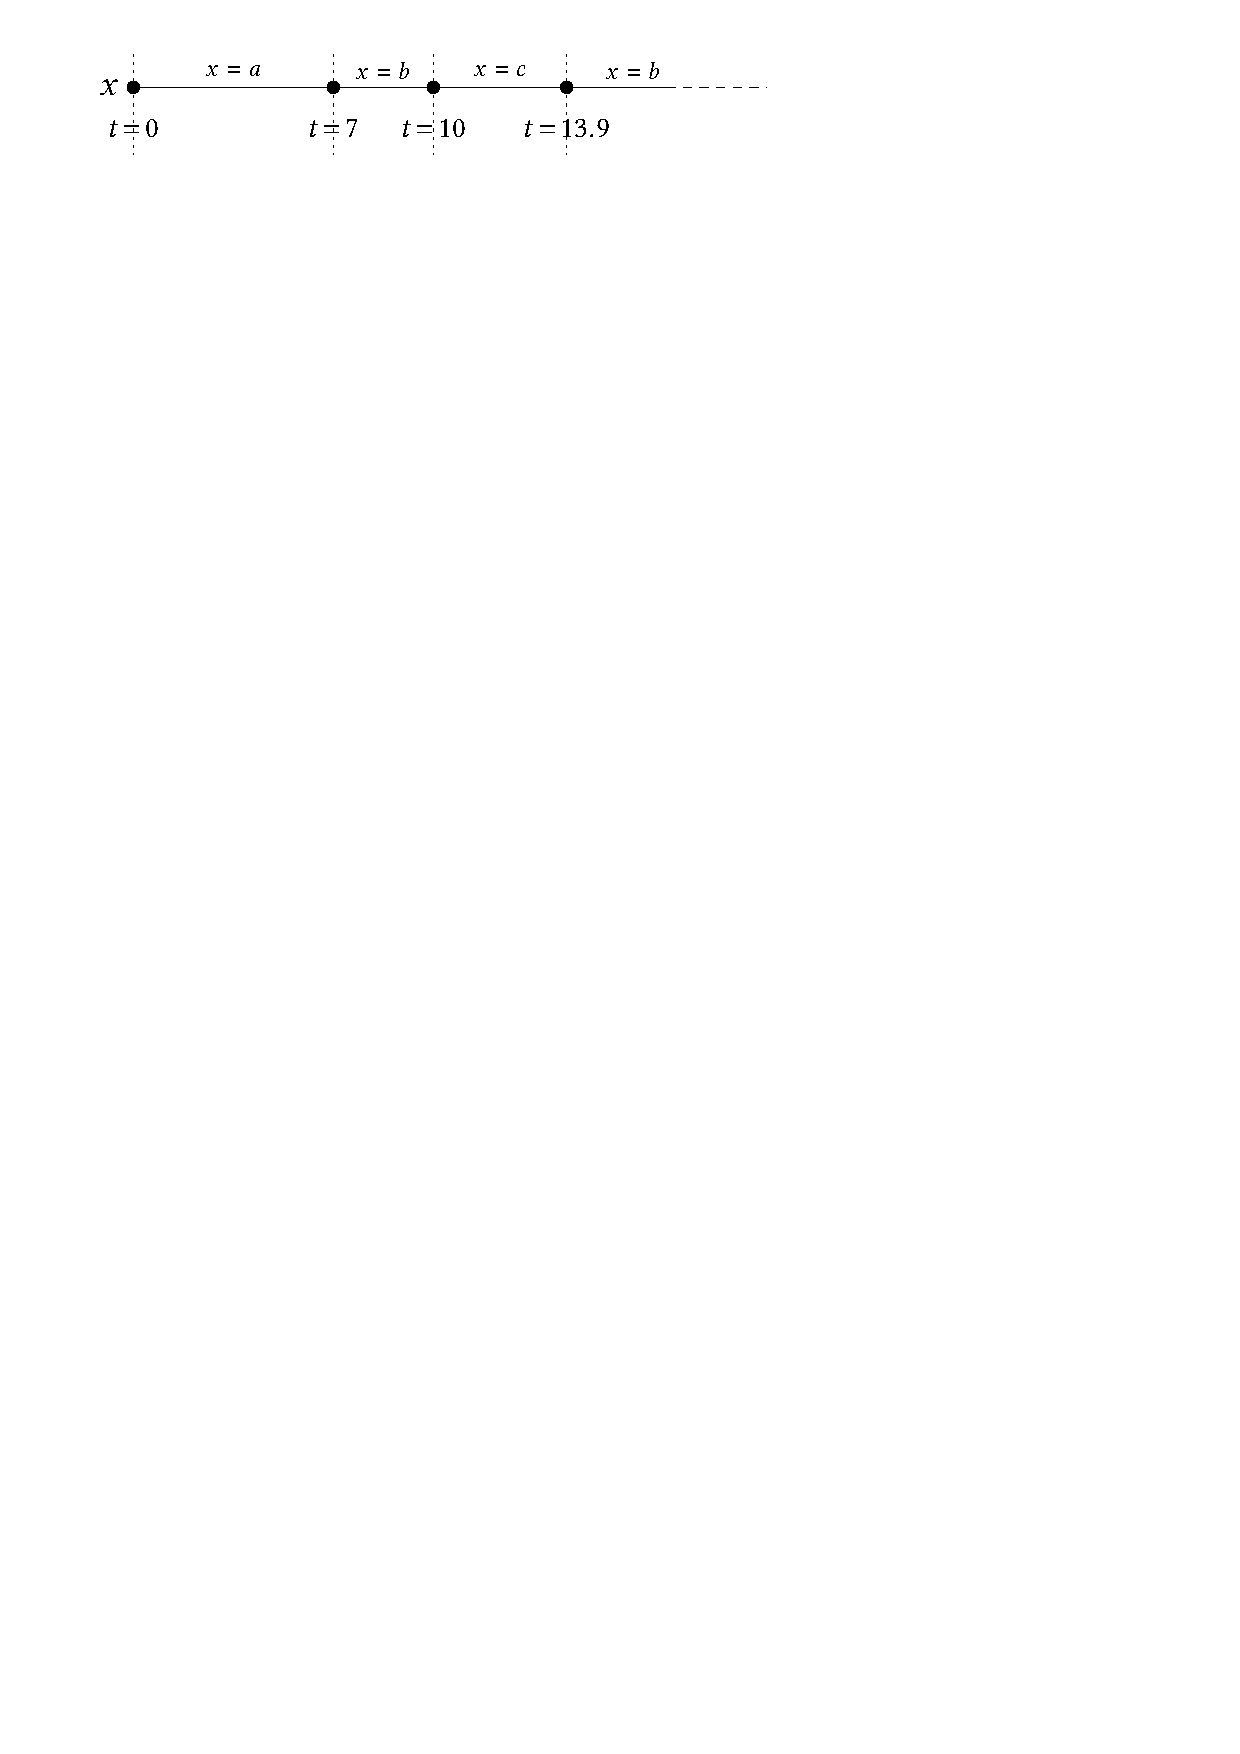
\includegraphics[scale=0.7]{Chaps/Timelines/timelineFig0.pdf}
    \caption{An example of timeline $(a,7)(b,3)(c,3.9)\cdots$ for the state variable $x= (V_x,T_x,D_x)$, where $V_x=\{a,b,c,\ldots\}$, $b\in T_x(a)$, $c\in T_x(b)$, $b\in T_x(c)$\dots\ and $D_x(a)=[5,8]$, $D_x(b)=[1,4]$, $D_x(c)=[2,\infty[$\dots}
    \label{fig:timelineEx}
\end{figure}

Given a finite set $SV$ of state variables, a \emph{multi-timeline} of $SV$ is a mapping $\Pi$ assigning to
each state variable $x\in SV$ a timeline for $x$.

Multi-timelines of $SV$ can be constrained by a set of \emph{synchronization
rules}, which relate tokens, possibly belonging to different timelines, through
temporal constraints on the start/end times of tokens (time-point constraints) and on the difference
between start/end times of tokens (interval constraints). The synchronization rules exploit
an alphabet $\Sigma=\{o,o_0,o_1,o_2,\ldots\}$ of token names to refer to the tokens along a multi-timeline, and are based on the notions of
\emph{atom} and \emph{existential statement}.

\begin{definition}[Atom]
  \label{def:timelines:atom}
  An \emph{atom} $\rho$ is either a clause of the form \mbox{$o_1\leq^{e_1,e_2}_{I} o_2$}
  (\emph{interval atom}), or of the forms $o_1\leq^{e_1}_{I} n$ or  $n\leq^{e_1}_{I}
  o_1$ (\emph{time-point atom}), where $o_1,o_2\in\Sigma$, $I\in\Intv$, $n\in\Nat$, and $e_1,e_2\in\{\start,\Ending\}$.
\end{definition}

An atom $\rho$ is evaluated with respect to a \emph{$\Sigma$-assignment $\lambda_\Pi$} for a given multi-timeline $\Pi$,
which is a mapping assigning to each token name $o\in \Sigma$ a pair $\lambda_\Pi(o)=(\pi,i)$ such that $\pi$ is a timeline of $\Pi$ and $0\leq i<|\pi|$ is a position along $\pi$ (intuitively,
$(\pi,i)$ represents the token of $\Pi$ referenced by the name $o$).

An interval atom $o_1\leq^{e_1,e_2}_{I} o_2$  \emph{is satisfied by  $\lambda_\Pi$} if $e_2(\lambda_\Pi(o_2))-e_1(\lambda_\Pi(o_1))\in I$.
A point atom $o\leq^{e}_{I} n$  (respectively, $n\leq^{e}_{I}o$)   \emph{is satisfied by  $\lambda_\Pi$} if $n-e(\lambda_\Pi(o))\in I$ (respectively, $e(\lambda_\Pi(o))-n\in I$).

\begin{definition}[Existential statement]
 An \emph{existential statement} $\mathcal{E}$ for a finite set $SV$ of state variables is a statement of the form
\[
\mathcal{E}=  \exists o_1[x_1=v_1]\cdots \exists o_n[x_n=v_n].\mathcal{C},
\]
  where $\mathcal{C}$ %$\mathcal{C}=\rho_0\land\ldots\land\rho_m$
  is a conjunction of atoms,
  $o_i\!\in\!\Sigma$, $x_i\!\in\! SV$, $v_i\!\in\! V_{x_i}$, for
  $1\leq i\leq n$. 

The elements $o_i[x_i=v_i]$ are called
  \emph{quantifiers}. A token name used in $\mathcal{C}$, but not occurring in any
  quantifier, is said to be \emph{free}. 
\end{definition}

  Given a $\Sigma$-assignment $\lambda_\Pi$ for a multi-timeline $\Pi$ of $SV$,
  we say that \emph{$\lambda_\Pi$ is consistent with the existential statement $\mathcal{E}$} if, for each quantifier $o_i[x_i=v_i]$, we have
   $\lambda_\Pi(o_i)=(\pi,h)$, where $\pi=\Pi(x_i)$ and the $h$-th token of $\pi$ has value $v_i$. A multi-timeline $\Pi$ of $SV$ \emph{satisfies} $\mathcal{E}$
   if there exists a $\Sigma$-assignment $\lambda_\Pi$ for $\Pi$ consistent with $\mathcal{E}$ such that each atom in $\mathcal{C}$ is satisfied by
   $\lambda_\Pi$.

We can now introduce synchronization rules, which constrain tokens, possibly belonging to different timelines.
\begin{definition}[Synchronization rule]
  A \emph{synchronization rule} $\mathcal{R}$ for a finite set $SV$ of state variables is a rule of one of the forms
  \[
  o_0[x_0=v_0] \to \mathcal{E}_1\lor \mathcal{E}_2\lor \ldots \lor \mathcal{E}_k, \qquad
          \true \to \mathcal{E}_1\lor \mathcal{E}_2\lor \ldots \lor \mathcal{E}_k,
  \]
  where $o_0\in\Sigma$, $x_0\in SV$, $v_0\in V_{x_0}$, and $\mathcal{E}_1, \ldots, \mathcal{E}_k$
  are \emph{existential statements}. % where only $o_0$ may appear free.
  In rules of the first
  form (which are called \emph{trigger rules}), the quantifier $o_0[x_0=v_0]$ is called \emph{trigger}; we require that only $o_0$ may appear free in $\mathcal{E}_i$, for all $1\leq i\leq n$. In rules of the second form (\emph{trigger-less rules}), we require
  that no token name appears free.
  \newline
  A trigger rule $\mathcal{R}$ is \emph{simple} if, for each existential statement $\mathcal{E}$ of $\mathcal{R}$ and each token name $o$ distinct from the trigger, there is at most one \emph{interval atom}
  of $\mathcal{E}$ where $o$ occurs.
\end{definition}

Intuitively, the  trigger $o_0[x_0=v_0]$ acts as a universal quantifier, which
states that \emph{for all} the tokens of the timeline for
$x_0$, where $x_0$ takes the
value $v_0$, at least one of the existential statements $\mathcal{E}_i$ must be satisfied. 
As an example, \[o_0[x_0=v_0]\to \exists o_1[x_1=v_1].o_0\leq^{\mathsf{e},\mathsf{s}}_{[2,\infty[} o_1\] states that after \emph{every} token for $x_0$ with value $v_0$ there exists a token for $x_1$ with value $v_1$ \emph{starting} at least 2 time instants after the \emph{end} of the former.
Trigger-less rules simply assert the
satisfaction of some existential statement. The intuitive meaning of \emph{simple} trigger rules is that they disallow simultaneous comparisons of multiple time-events
 (start/end times of tokens) with a non-trigger reference time-event. 
 
 The semantics of synchronization rules is formally defined as follows.
\begin{definition}[Semantics of synchronization rules]\label{def:semanticsRules}
Let $\Pi$ be a multi-timeline of a set $SV$ of state variables.

Given a \emph{trigger-less rule} $\mathcal{R}$ of $SV$, \emph{$\Pi$ satisfies $\mathcal{R}$} if $\Pi$ satisfies some existential statement of $\mathcal{R}$.

Given a \emph{trigger rule} $\mathcal{R}$ of $SV$ with trigger $o_0[x_0=v_0]$, \emph{$\Pi$ satisfies   $\mathcal{R}$} if, for every position $i$ of the
 timeline $\pi=\Pi(x_0)$ for $x_0$ such that $\pi(i)=(v_0,d)$, there exists an existential statement $\mathcal{E}$ of $\mathcal{R}$  and a $\Sigma$-assignment
 $\lambda_\Pi$ for $\Pi$ consistent with $\mathcal{E}$ such that $\lambda_\Pi(o_0)= (\pi,i)$ and $\lambda_\Pi$ satisfies all the atoms of $\mathcal{E}$.
\end{definition}

In the paper, we shall also focus on a stronger notion of satisfaction of trigger rules, called \emph{satisfaction under the future semantics}: it requires that all non-trigger tokens selected by some quantifier
%in the selected existential statements compared with the trigger token
do not start \emph{strictly before} the start time of the trigger token.

\begin{definition}[Future semantics of trigger rules]\label{def:futurerules}
  A multi-timeline $\Pi$ of $SV$ satisfies a trigger rule \[\mathcal{R}= o_0[x_0=v_0] \to \mathcal{E}_1\vee \mathcal{E}_2\vee
  \ldots \vee \mathcal{E}_k\]   \emph{under the future semantics} if $\Pi$ satisfies the trigger rule obtained from
  $\mathcal{R}$ by replacing each existential statement \[\mathcal{E}_i=\exists o_1[x_1=v_1]\cdots \exists o_n[x_n=v_n].\mathcal{C}\]
  by \[\mathcal{E}_i'=\exists o_1[x_1=v_1]\cdots \exists o_n[x_n=v_n].\Big(\mathcal{C}\wedge  \bigwedge_{i=1}^{n} o_0\leq^{\start,\start}_{[0,+\infty[} o_i\Big).\]
\end{definition}

A \emph{TP domain} $P=(SV,R)$ is specified by a finite set $SV$ of state variables and
a finite set $R$ of synchronization rules for $SV$ modeling their admissible behaviors.
Trigger-less rules can be used to express initial, as well as intermediate conditions
and the goals of the problem, while trigger rules are much more powerful and useful, for instance, to specify invariants and response requirements. 

A \emph{plan for $P=(SV,R)$} is a  multi-timeline of $SV$ satisfying all the rules in $R$. A \emph{future plan for $P$} is defined in a similar way, but we require satisfaction under the future semantics of \emph{all} trigger rules.

In the next sections we will study the following decision problems:
\begin{description}
  \item[TP problem] Given a TP domain $P=(SV,R)$, is there a plan for $P$?
  \item[Future TP problem] Given a TP domain $P\!=\!(SV\!,R)$, is there a \emph{future} plan for $P$?
\end{description}
%
%\begin{definition}%[Planning problem]
%  \label{def:timelines:problem}
%  A timeline-based planning \emph{problem} is a pair $P=(SV,S)$, where $SV$ is
%  a set of state variables and $S$ is a set of synchronization rules involving
%  variables in $SV$.
%  A \emph{plan} for
%  $P$ is a set of timelines $\Pi$, one for each $x_i\in SV$, such
%  that all the synchronization rules in $S$ are satisfied by the set $\Gamma$
%  of all tokens involved in (any of) the timelines of $\Pi$.
%\end{definition}

Table~\ref{tab:complex} summarizes all the decidability and complexity results described in the following about the mentioned problems:
we will consider mixes of restrictions on TP involving trigger rules with future semantics, simple trigger rules, and intervals in atoms (of trigger rules) which are non-singular or in $\Intv_{(0,\infty)}$.

\begin{table}[t]
    \centering    
    \caption{Decidability and complexity of restrictions of the TP problem.}
    \label{tab:complex}
    \resizebox{\linewidth}{!}{
    \begin{tabular}{r|c|c}
    	%\hline 
    	& TP problem & Future TP problem \\ 
    	\hline 
    	Unrestricted & Undecidable & (Decidable?) Non-primitive recursive-hard \\ 
    	\hline 
    	Simple trigger rules & Undecidable & Decidable (non-primitive recursive) \\ 
    	\hline 
    	Simple trigger rules, & \multirow{2}{*}{?} & \multirow{2}{*}{$\EXPSPACE$-complete} \\ 
    	non-singular intervals & & \\
    	\hline 
    	Simple trigger rules, & \multirow{2}{*}{?} & \multirow{2}{*}{$\Psp$-complete} \\ 
    	intervals in $\Intv_{(0,\infty)}$ & & \\
    	\hline 
    	Trigger-less rules only & $\NP$-complete & // \\ 
    	%\hline 
    \end{tabular} 
    }
\end{table}
                           % preliminary page info

%%%%%%%%%%%%%%%%%%%%%%%%%%%%%%%%%%%%%%%%%%%%%%%%%%%%%%%%%%%%%%%%%%%%%%%%
%                                                                      %
%                          PRELIMINARY PAGES                           %
%                                                                      %
%%%%%%%%%%%%%%%%%%%%%%%%%%%%%%%%%%%%%%%%%%%%%%%%%%%%%%%%%%%%%%%%%%%%%%%%

\title          {Improving the Throughput \\
                of Connectionless Datagram Protocols \\
                over Networks with Limited Bandwidth}
\author         {Richard Bert Wales}
\department     {Computer Science}
% Note:  degreeyear should be optional, but as of  5-Feb-96
% it seems required or you get a year of ``2''.   -johnh
\degreeyear     {1993}

%%%%%%%%%%%%%%%%%%%%%%%%%%%%%%%%%%%%%%%%%%%%%%%%%%%%%%%%%%%%%%%%%%%%%%%%

\chair          {Jack W.\ Carlyle}
\member         {Mario Gerla}
\member         {David G.\ Cantor}
\member         {Richard L.\ Baker}
\member         {Robert M.\ Stevenson}

%%%%%%%%%%%%%%%%%%%%%%%%%%%%%%%%%%%%%%%%%%%%%%%%%%%%%%%%%%%%%%%%%%%%%%%%

\dedication     {\textsl{To my mother \ldots \\
                who---among so many other things--- \\
                saw to it that I learned to touch-type \\
                while I was still in elementary school}}

%%%%%%%%%%%%%%%%%%%%%%%%%%%%%%%%%%%%%%%%%%%%%%%%%%%%%%%%%%%%%%%%%%%%%%%%

\acknowledgments {(Acknowledgments omitted for brevity.)}

%%%%%%%%%%%%%%%%%%%%%%%%%%%%%%%%%%%%%%%%%%%%%%%%%%%%%%%%%%%%%%%%%%%%%%%%

\vitaitem   {1952}
                {Born, San Francisco, California, USA.}
\vitaitem   {1974--1975}
                {Campus computer center ``User Services'' programmer and
                consultant, Stanford Center for Information Processing,
                Stanford University, Stanford, California.}
\vitaitem   {1974--1975}
                {Programmer, Housing Office, Stanford University.
                Designed a major software system for assigning
                students to on-campus housing.
                With some later improvements, it is still in use.}
\vitaitem   {1975}
                {B.S.~(Mathematics) and A.B.~(Music),
                Stanford University.}
\vitaitem   {1977}
                {M.A.~(Music), UCLA, Los Angeles, California.}
\vitaitem   {1977--1979}
                {Teaching Assistant, Computer Science Department, UCLA.
                Taught sections of Engineering 10 (beginning computer
                programming course) under direction of Professor Leon
                Levine.
                During summer 1979, taught a beginning programming
                course as part of the Freshman Summer Program.}
\vitaitem   {1979}
                {M.S.~(Computer Science), UCLA.}
\vitaitem   {1979--1980}
                {Teaching Assistant, Computer Science Department, UCLA.}
\vitaitem   {1980--1981}
                {Research Assistant, Computer Science Department, UCLA.}
\vitaitem   {1981--present}
                {Programmer/Analyst, Computer Science Department, UCLA.}

%%%%%%%%%%%%%%%%%%%%%%%%%%%%%%%%%%%%%%%%%%%%%%%%%%%%%%%%%%%%%%%%%%%%%%%%

\publication    {\textsl{MADHOUS Reference Manual.}
                Stanford University, Dean of Student Affairs
                (Residential Education Division), 1978.
                Technical documentation for the MADHOUS
                software system used to assign students to
                on-campus housing.}

%%%%%%%%%%%%%%%%%%%%%%%%%%%%%%%%%%%%%%%%%%%%%%%%%%%%%%%%%%%%%%%%%%%%%%%%

\abstract       {(Abstract omitted for brevity)}

%%%%%%%%%%%%%%%%%%%%%%%%%%%%%%%%%%%%%%%%%%%%%%%%%%%%%%%%%%%%%%%%%%%%%%%%



\begin {document}
\makeintropages

%%%%%%%%%%%%%%%%%%%%%%%%%%%%%%%%%%%%%%%%%%%%%%%%%%%%%%%%%%%%%%%%%%%%%%
%
% Ordinarily each chapter (at least) is in a separate file.
%
%\begin{savequote}[75mm]
Nulla facilisi. In vel sem. Morbi id urna in diam dignissim feugiat. Proin molestie tortor eu velit. Aliquam erat volutpat. Nullam ultrices, diam tempus vulputate egestas, eros pede varius leo.
\qauthor{Quoteauthor Lastname}
\end{savequote}

\chapter{The title of chapter one}

\newthought{There's something to be said} for having a good opening line. Morbi commodo, ipsum sed pharetra gravida, orci  $x = 1/\alpha$ magna rhoncus neque, id pulvinar odio lorem non turpis \cite{Eigen1971, Knuth1968}. Nullam sit amet enim. Suspendisse id velit vitae ligula volutpat condimentum. Aliquam erat volutpat. Sed quis velit. Nulla facilisi. Nulla libero. Vivamus pharetra posuere sapien. Nam consectetuer. Sed aliquam, nunc eget euismod ullamcorper, lectus nunc ullamcorper orci, fermentum bibendum enim nibh eget ipsum. Donec porttitor ligula eu dolor. Maecenas vitae nulla consequat libero cursus venenatis. Nam magna enim, accumsan eu, blandit sed, blandit a, eros.
$$\zeta = \frac{1039}{\pi}$$


% For an example of a full page figure, see Fig.~\ref{fig:myFullPageFigure}.

Lorem ipsum dolor sit amet, consectetuer adipiscing elit. Morbi commodo, ipsum sed pharetra gravida, orci magna rhoncus neque, id pulvinar odio lorem non turpis. Nullam sit amet enim. Suspendisse id velit vitae ligula volutpat condimentum. Aliquam erat volutpat. Sed quis velit. Nulla facilisi. Nulla libero. Vivamus pharetra posuere sapien. Nam consectetuer. Sed aliquam, nunc eget euismod ullamcorper, lectus nunc ullamcorper orci, fermentum bibendum enim nibh eget ipsum. Donec porttitor ligula eu dolor. Maecenas vitae nulla consequat libero cursus venenatis. Nam magna enim, accumsan eu, blandit sed, blandit a, eros.

Quisque facilisis erat a dui. Nam malesuada ornare dolor. Cras gravida, diam sit amet rhoncus ornare, erat elit consectetuer erat, id egestas pede nibh eget odio. Proin tincidunt, velit vel porta elementum, magna diam molestie sapien, non aliquet massa pede eu diam. Aliquam iaculis. Fusce et ipsum et nulla tristique facilisis. Donec eget sem sit amet ligula viverra gravida. Etiam vehicula urna vel turpis. Suspendisse sagittis ante a urna. Morbi a est quis orci consequat rutrum. Nullam egestas feugiat felis. Integer adipiscing semper ligula. Nunc molestie, nisl sit amet cursus convallis, sapien lectus pretium metus, vitae pretium enim wisi id lectus. Donec vestibulum. Etiam vel nibh. Nulla facilisi. Mauris pharetra. Donec augue. Fusce ultrices, neque id dignissim ultrices, tellus mauris dictum elit, vel lacinia enim metus eu nunc.

Pellentesque habitant morbi tristique senectus et netus et malesuada fames ac turpis egestas. Vestibulum tortor quam, feugiat vitae, ultricies eget, tempor sit amet, ante. Donec eu libero sit amet quam egestas semper. Aenean ultricies mi vitae est. Mauris placerat eleifend leo. Quisque sit amet est et sapien ullamcorper pharetra. Vestibulum erat wisi, condimentum sed, commodo vitae, ornare sit amet, wisi. Aenean fermentum, elit eget tincidunt condimentum, eros ipsum rutrum orci, sagittis tempus lacus enim ac dui. Donec non enim in turpis pulvinar facilisis. Ut felis.

Cras sed ante. Phasellus in massa. Curabitur dolor eros, gravida et, hendrerit ac, cursus non, massa. Aliquam lorem. In hac habitasse platea dictumst. Cras eu mauris. Quisque lacus. Donec ipsum. Nullam vitae sem at nunc pharetra ultricies. Vivamus elit eros, ullamcorper a, adipiscing sit amet, porttitor ut, nibh. Maecenas adipiscing mollis massa. Nunc ut dui eget nulla venenatis aliquet. Sed luctus posuere justo. Cras vehicula varius turpis. Vivamus eros metus, tristique sit amet, molestie dignissim, malesuada et, urna.

Cras dictum. Maecenas ut turpis. In vitae erat ac orci dignissim eleifend. Nunc quis justo. Sed vel ipsum in purus tincidunt pharetra. Sed pulvinar, felis id consectetuer malesuada, enim nisl mattis elit, a facilisis tortor nibh quis leo. Sed augue lacus, pretium vitae, molestie eget, rhoncus quis, elit. Donec in augue. Fusce orci wisi, ornare id, mollis vel, lacinia vel, massa.

Lorem ipsum dolor sit amet, consectetuer adipiscing elit. Morbi commodo, ipsum sed pharetra gravida, orci magna rhoncus neque, id pulvinar odio lorem non turpis. Nullam sit amet enim. Suspendisse id velit vitae ligula volutpat condimentum. Aliquam erat volutpat. Sed quis velit. Nulla facilisi. Nulla libero. Vivamus pharetra posuere sapien. Nam consectetuer. Sed aliquam, nunc eget euismod ullamcorper, lectus nunc ullamcorper orci, fermentum bibendum enim nibh eget ipsum. Donec porttitor ligula eu dolor. Maecenas vitae nulla consequat libero cursus venenatis. Nam magna enim, accumsan eu, blandit sed, blandit a, eros.

Quisque facilisis erat a dui. Nam malesuada ornare dolor. Cras gravida, diam sit amet rhoncus ornare, erat elit consectetuer erat, id egestas pede nibh eget odio. Proin tincidunt, velit vel porta elementum, magna diam molestie sapien, non aliquet massa pede eu diam. Aliquam iaculis. Fusce et ipsum et nulla tristique facilisis. Donec eget sem sit amet ligula viverra gravida. Etiam vehicula urna vel turpis. Suspendisse sagittis ante a urna. Morbi a est quis orci consequat rutrum. Nullam egestas feugiat felis. Integer adipiscing semper ligula. Nunc molestie, nisl sit amet cursus convallis, sapien lectus pretium metus, vitae pretium enim wisi id lectus. Donec vestibulum. Etiam vel nibh. Nulla facilisi. Mauris pharetra. Donec augue. Fusce ultrices, neque id dignissim ultrices, tellus mauris dictum elit, vel lacinia enim metus eu nunc.

\texttt{This is a line of code.}

Proin at eros non eros adipiscing mollis. Donec semper turpis sed diam. Sed consequat ligula nec tortor. Integer eget sem. Ut vitae enim eu est vehicula gravida. Morbi ipsum ipsum, porta nec, tempor id, auctor vitae, purus. Pellentesque neque. Nulla luctus erat vitae libero. Integer nec enim. Phasellus aliquam enim et tortor. Quisque aliquet, quam elementum condimentum feugiat, tellus odio consectetuer wisi, vel nonummy sem neque in elit. Curabitur eleifend wisi iaculis ipsum. Pellentesque habitant morbi tristique senectus et netus et malesuada fames ac turpis egestas. In non velit non ligula laoreet ultrices. Praesent ultricies facilisis nisl. Vivamus luctus elit sit amet mi. Phasellus pellentesque, erat eget elementum volutpat, dolor nisl porta neque, vitae sodales ipsum nibh in ligula. Maecenas mattis pulvinar diam. Curabitur sed leo.

Nulla facilisi. In vel sem. Morbi id urna in diam dignissim feugiat. Proin molestie tortor eu velit. Aliquam erat volutpat. Nullam ultrices, diam tempus vulputate egestas, eros pede varius leo, sed imperdiet lectus est ornare odio. Lorem ipsum dolor sit amet, consectetuer adipiscing elit. Proin consectetuer velit in dui. Phasellus wisi purus, interdum vitae, rutrum accumsan, viverra in, velit. Sed enim risus, congue non, tristique in, commodo eu, metus. Aenean tortor mi, imperdiet id, gravida eu, posuere eu, felis. Mauris sollicitudin, turpis in hendrerit sodales, lectus ipsum pellentesque ligula, sit amet scelerisque urna nibh ut arcu. Aliquam in lacus. Vestibulum ante ipsum primis in faucibus orci luctus et ultrices posuere cubilia Curae; Nulla placerat aliquam wisi. Mauris viverra odio. Quisque fermentum pulvinar odio. Proin posuere est vitae ligula. Etiam euismod. Cras a eros.

Nunc auctor bibendum eros. Maecenas porta accumsan mauris. Etiam enim enim, elementum sed, bibendum quis, rhoncus non, metus. Fusce neque dolor, adipiscing sed, consectetuer et, lacinia sit amet, quam. Suspendisse wisi quam, consectetuer in, blandit sed, suscipit eu, eros. Etiam ligula enim, tempor ut, blandit nec, mollis eu, lectus. Nam cursus. Vivamus iaculis. Aenean risus purus, pharetra in, blandit quis, gravida a, turpis. Donec nisl. Aenean eget mi. Fusce mattis est id diam. Phasellus faucibus interdum sapien. Duis quis nunc. Sed enim.

Pellentesque vel dui sed orci faucibus iaculis. Suspendisse dictum magna id purus tincidunt rutrum. Nulla congue. Vivamus sit amet lorem posuere dui vulputate ornare. Phasellus mattis sollicitudin ligula. Duis dignissim felis et urna. Integer adipiscing congue metus. Nam pede. Etiam non wisi. Sed accumsan dolor ac augue. Pellentesque eget lectus. Aliquam nec dolor nec tellus ornare venenatis. Nullam blandit placerat sem. Curabitur quis ipsum. Mauris nisl tellus, aliquet eu, suscipit eu, ullamcorper quis, magna. Mauris elementum, pede at sodales vestibulum, nulla tortor congue massa, quis pellentesque odio dui id est. Cras faucibus augue.

Suspendisse vestibulum dignissim quam. Integer vel augue. Phasellus nulla purus, interdum ac, venenatis non, varius rutrum, leo. Pellentesque habitant morbi tristique senectus et netus et malesuada fames ac turpis egestas. Duis a eros. Class aptent taciti sociosqu ad litora torquent per conubia nostra, per inceptos hymenaeos. Fusce magna mi, porttitor quis, convallis eget, sodales ac, urna. Phasellus luctus venenatis magna. Vivamus eget lacus. Nunc tincidunt convallis tortor. Duis eros mi, dictum vel, fringilla sit amet, fermentum id, sem. Phasellus nunc enim, faucibus ut, laoreet in, consequat id, metus. Vivamus dignissim. Cras lobortis tempor velit. Phasellus nec diam ac nisl lacinia tristique. Nullam nec metus id mi dictum dignissim. Nullam quis wisi non sem lobortis condimentum. Phasellus pulvinar, nulla non aliquam eleifend, tortor wisi scelerisque felis, in sollicitudin arcu ante lacinia leo.

Pellentesque habitant morbi tristique senectus et netus et malesuada fames ac turpis egestas. Vestibulum tortor quam, feugiat vitae, ultricies eget, tempor sit amet, ante. Donec eu libero sit amet quam egestas semper. Aenean ultricies mi vitae est. Mauris placerat eleifend leo. Quisque sit amet est et sapien ullamcorper pharetra. Vestibulum erat wisi, condimentum sed, commodo vitae, ornare sit amet, wisi. Aenean fermentum, elit eget tincidunt condimentum, eros ipsum rutrum orci, sagittis tempus lacus enim ac dui. Donec non enim in turpis pulvinar facilisis. Ut felis.

Cras sed ante. Phasellus in massa. Curabitur dolor eros, gravida et, hendrerit ac, cursus non, massa. Aliquam lorem. In hac habitasse platea dictumst. Cras eu mauris. Quisque lacus. Donec ipsum. Nullam vitae sem at nunc pharetra ultricies. Vivamus elit eros, ullamcorper a, adipiscing sit amet, porttitor ut, nibh. Maecenas adipiscing mollis massa. Nunc ut dui eget nulla venenatis aliquet. Sed luctus posuere justo. Cras vehicula varius turpis. Vivamus eros metus, tristique sit amet, molestie dignissim, malesuada et, urna.

Cras dictum. Maecenas ut turpis. In vitae erat ac orci dignissim eleifend. Nunc quis justo. Sed vel ipsum in purus tincidunt pharetra. Sed pulvinar, felis id consectetuer malesuada, enim nisl mattis elit, a facilisis tortor nibh quis leo. Sed augue lacus, pretium vitae, molestie eget, rhoncus quis, elit. Donec in augue. Fusce orci wisi, ornare id, mollis vel, lacinia vel, massa.

Lorem ipsum dolor sit amet, consectetuer adipiscing elit. Morbi commodo, ipsum sed pharetra gravida, orci magna rhoncus neque, id pulvinar odio lorem non turpis. Nullam sit amet enim. Suspendisse id velit vitae ligula volutpat condimentum. Aliquam erat volutpat. Sed quis velit. Nulla facilisi. Nulla libero. Vivamus pharetra posuere sapien. Nam consectetuer. Sed aliquam, nunc eget euismod ullamcorper, lectus nunc ullamcorper orci, fermentum bibendum enim nibh eget ipsum. Donec porttitor ligula eu dolor. Maecenas vitae nulla consequat libero cursus venenatis. Nam magna enim, accumsan eu, blandit sed, blandit a, eros.


\begin{figure}
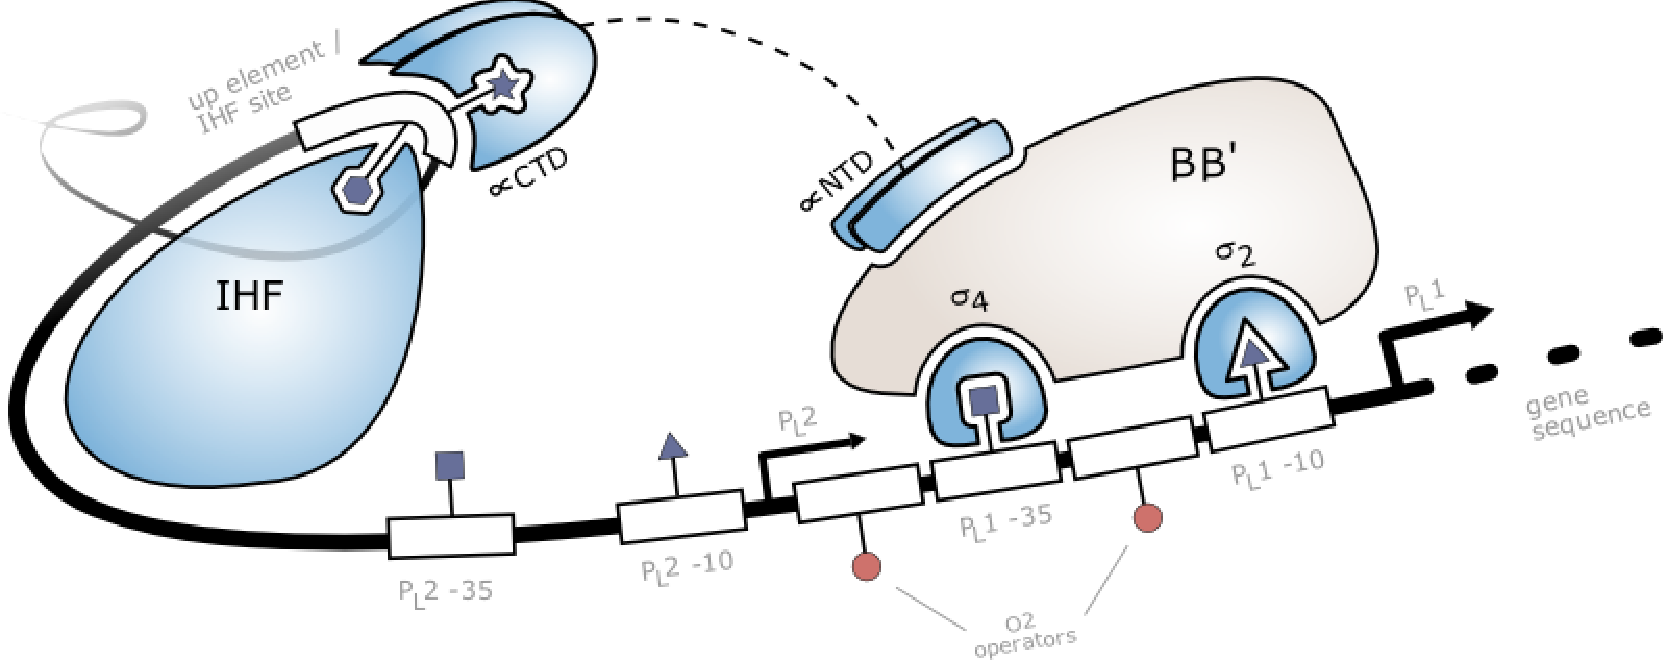
\includegraphics[width=\textwidth]{figures/fig1}
\caption[Short figure name.]{This is a figure that floats inline and here is its caption.
\label{fig:myInlineFigure}}
\end{figure}


Quisque facilisis erat a dui. Nam malesuada ornare dolor. Cras gravida, diam sit amet rhoncus ornare, erat elit consectetuer erat, id egestas pede nibh eget odio. Proin tincidunt, velit vel porta elementum, magna diam molestie sapien, non aliquet massa pede eu diam. Aliquam iaculis. Fusce et ipsum et nulla tristique facilisis. Donec eget sem sit amet ligula viverra gravida. Etiam vehicula urna vel turpis. Suspendisse sagittis ante a urna. Morbi a est quis orci consequat rutrum. Nullam egestas feugiat felis. Integer adipiscing semper ligula. Nunc molestie, nisl sit amet cursus convallis, sapien lectus pretium metus, vitae pretium enim wisi id lectus. Donec vestibulum. Etiam vel nibh. Nulla facilisi. Mauris pharetra. Donec augue. Fusce ultrices, neque id dignissim ultrices, tellus mauris dictum elit, vel lacinia enim metus eu nunc.

Proin at eros non eros adipiscing mollis. Donec semper turpis sed diam. Sed consequat ligula nec tortor. Integer eget sem. Ut vitae enim eu est vehicula gravida. Morbi ipsum ipsum, porta nec, tempor id, auctor vitae, purus. Pellentesque neque. Nulla luctus erat vitae libero. Integer nec enim. Phasellus aliquam enim et tortor. Quisque aliquet, quam elementum condimentum feugiat, tellus odio consectetuer wisi, vel nonummy sem neque in elit. Curabitur eleifend wisi iaculis ipsum. Pellentesque habitant morbi tristique senectus et netus et malesuada fames ac turpis egestas. In non velit non ligula laoreet ultrices. Praesent ultricies facilisis nisl. Vivamus luctus elit sit amet mi. Phasellus pellentesque, erat eget elementum volutpat, dolor nisl porta neque, vitae sodales ipsum nibh in ligula. Maecenas mattis pulvinar diam. Curabitur sed leo.

Nulla facilisi. In vel sem. Morbi id urna in diam dignissim feugiat. Proin molestie tortor eu velit. Aliquam erat volutpat. Nullam ultrices, diam tempus vulputate egestas, eros pede varius leo, sed imperdiet lectus est ornare odio. Lorem ipsum dolor sit amet, consectetuer adipiscing elit. Proin consectetuer velit in dui. Phasellus wisi purus, interdum vitae, rutrum accumsan, viverra in, velit. Sed enim risus, congue non, tristique in, commodo eu, metus. Aenean tortor mi, imperdiet id, gravida eu, posuere eu, felis. Mauris sollicitudin, turpis in hendrerit sodales, lectus ipsum pellentesque ligula, sit amet scelerisque urna nibh ut arcu. Aliquam in lacus. Vestibulum ante ipsum primis in faucibus orci luctus et ultrices posuere cubilia Curae; Nulla placerat aliquam wisi. Mauris viverra odio. Quisque fermentum pulvinar odio. Proin posuere est vitae ligula. Etiam euismod. Cras a eros.

Nunc auctor bibendum eros. Maecenas porta accumsan mauris. Etiam enim enim, elementum sed, bibendum quis, rhoncus non, metus. Fusce neque dolor, adipiscing sed, consectetuer et, lacinia sit amet, quam. Suspendisse wisi quam, consectetuer in, blandit sed, suscipit eu, eros. Etiam ligula enim, tempor ut, blandit nec, mollis eu, lectus. Nam cursus. Vivamus iaculis. Aenean risus purus, pharetra in, blandit quis, gravida a, turpis. Donec nisl. Aenean eget mi. Fusce mattis est id diam. Phasellus faucibus interdum sapien. Duis quis nunc. Sed enim.

Pellentesque vel dui sed orci faucibus iaculis. Suspendisse dictum magna id purus tincidunt rutrum. Nulla congue. Vivamus sit amet lorem posuere dui vulputate ornare. Phasellus mattis sollicitudin ligula. Duis dignissim felis et urna. Integer adipiscing congue metus. Nam pede. Etiam non wisi. Sed accumsan dolor ac augue. Pellentesque eget lectus. Aliquam nec dolor nec tellus ornare venenatis. Nullam blandit placerat sem. Curabitur quis ipsum. Mauris nisl tellus, aliquet eu, suscipit eu, ullamcorper quis, magna. Mauris elementum, pede at sodales vestibulum, nulla tortor congue massa, quis pellentesque odio dui id est. Cras faucibus augue.

%% Requires fltpage2 package
%%
% \begin{FPfigure}
% 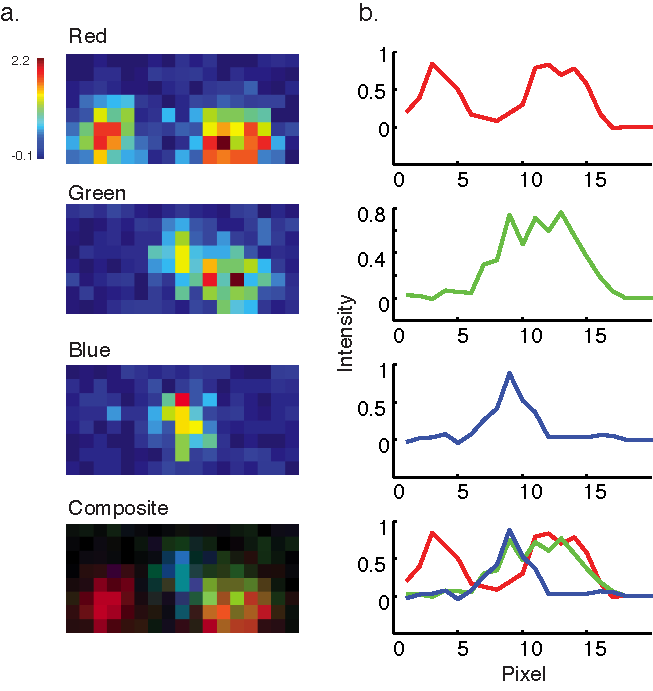
\includegraphics[width=\textwidth]{figures/fullpage}
% \caption[Short figure name.]{This is a full page figure using the FPfigure command. It takes up the whole page and the caption appears on the preceding page. Its useful for large figures. Harvard's rules about full page figures are tricky, but you don't have to worry about it because we took care of it for you. For example, the full figure is supposed to have a title in the same style as the caption but without the actual caption. The caption is supposed to appear alone on the preceding page with no other text. You do't have to worry about any of that. We have modified the fltpage package to make it work. This is a lengthy caption and it clearly would not fit on the same page as the figure. Note that you should only use the FPfigure command in instances where the figure really is too large. If the figure is small enough to fit by the caption than it does not produce the desired effect. Good luck with your thesis. I have to keep writing this to make the caption really long. LaTex is a lot of fun. You will enjoy working with it. Good luck on your post doctoral life! I am looking forward to mine. \label{fig:myFullPageFigure}}
% \end{FPfigure}
% \afterpage{\clearpage}

Suspendisse vestibulum dignissim quam. Integer vel augue. Phasellus nulla purus, interdum ac, venenatis non, varius rutrum, leo. Pellentesque habitant morbi tristique senectus et netus et malesuada fames ac turpis egestas. Duis a eros. Class aptent taciti sociosqu ad litora torquent per conubia nostra, per inceptos hymenaeos. Fusce magna mi, porttitor quis, convallis eget, sodales ac, urna. Phasellus luctus venenatis magna. Vivamus eget lacus. Nunc tincidunt convallis tortor. Duis eros mi, dictum vel, fringilla sit amet, fermentum id, sem. Phasellus nunc enim, faucibus ut, laoreet in, consequat id, metus. Vivamus dignissim. Cras lobortis tempor velit. Phasellus nec diam ac nisl lacinia tristique. Nullam nec metus id mi dictum dignissim. Nullam quis wisi non sem lobortis condimentum. Phasellus pulvinar, nulla non aliquam eleifend, tortor wisi scelerisque felis, in sollicitudin arcu ante lacinia leo.

Pellentesque habitant morbi tristique senectus et netus et malesuada fames ac turpis egestas. Vestibulum tortor quam, feugiat vitae, ultricies eget, tempor sit amet, ante. Donec eu libero sit amet quam egestas semper. Aenean ultricies mi vitae est. Mauris placerat eleifend leo. Quisque sit amet est et sapien ullamcorper pharetra. Vestibulum erat wisi, condimentum sed, commodo vitae, ornare sit amet, wisi. Aenean fermentum, elit eget tincidunt condimentum, eros ipsum rutrum orci, sagittis tempus lacus enim ac dui. Donec non enim in turpis pulvinar facilisis. Ut felis.

Cras sed ante. Phasellus in massa. Curabitur dolor eros, gravida et, hendrerit ac, cursus non, massa. Aliquam lorem. In hac habitasse platea dictumst. Cras eu mauris. Quisque lacus. Donec ipsum. Nullam vitae sem at nunc pharetra ultricies. Vivamus elit eros, ullamcorper a, adipiscing sit amet, porttitor ut, nibh. Maecenas adipiscing mollis massa. Nunc ut dui eget nulla venenatis aliquet. Sed luctus posuere justo. Cras vehicula varius turpis. Vivamus eros metus, tristique sit amet, molestie dignissim, malesuada et, urna.

Proin at eros non eros adipiscing mollis. Donec semper turpis sed diam. Sed consequat ligula nec tortor. Integer eget sem. Ut vitae enim eu est vehicula gravida. Morbi ipsum ipsum, porta nec, tempor id, auctor vitae, purus. Pellentesque neque. Nulla luctus erat vitae libero. Integer nec enim. Phasellus aliquam enim et tortor. Quisque aliquet, quam elementum condimentum feugiat, tellus odio consectetuer wisi, vel nonummy sem neque in elit. Curabitur eleifend wisi iaculis ipsum. Pellentesque habitant morbi tristique senectus et netus et malesuada fames ac turpis egestas. In non velit non ligula laoreet ultrices. Praesent ultricies facilisis nisl. Vivamus luctus elit sit amet mi. Phasellus pellentesque, erat eget elementum volutpat, dolor nisl porta neque, vitae sodales ipsum nibh in ligula. Maecenas mattis pulvinar diam. Curabitur sed leo.

Nulla facilisi. In vel sem. Morbi id urna in diam dignissim feugiat. Proin molestie tortor eu velit. Aliquam erat volutpat. Nullam ultrices, diam tempus vulputate egestas, eros pede varius leo, sed imperdiet lectus est ornare odio. Lorem ipsum dolor sit amet, consectetuer adipiscing elit. Proin consectetuer velit in dui. Phasellus wisi purus, interdum vitae, rutrum accumsan, viverra in, velit. Sed enim risus, congue non, tristique in, commodo eu, metus. Aenean tortor mi, imperdiet id, gravida eu, posuere eu, felis. Mauris sollicitudin, turpis in hendrerit sodales, lectus ipsum pellentesque ligula, sit amet scelerisque urna nibh ut arcu. Aliquam in lacus. Vestibulum ante ipsum primis in faucibus orci luctus et ultrices posuere cubilia Curae; Nulla placerat aliquam wisi. Mauris viverra odio. Quisque fermentum pulvinar odio. Proin posuere est vitae ligula. Etiam euismod. Cras a eros.

Nunc auctor bibendum eros. Maecenas porta accumsan mauris. Etiam enim enim, elementum sed, bibendum quis, rhoncus non, metus. Fusce neque dolor, adipiscing sed, consectetuer et, lacinia sit amet, quam. Suspendisse wisi quam, consectetuer in, blandit sed, suscipit eu, eros. Etiam ligula enim, tempor ut, blandit nec, mollis eu, lectus. Nam cursus. Vivamus iaculis. Aenean risus purus, pharetra in, blandit quis, gravida a, turpis. Donec nisl. Aenean eget mi. Fusce mattis est id diam. Phasellus faucibus interdum sapien. Duis quis nunc. Sed enim.

Pellentesque vel dui sed orci faucibus iaculis. Suspendisse dictum magna id purus tincidunt rutrum. Nulla congue. Vivamus sit amet lorem posuere dui vulputate ornare. Phasellus mattis sollicitudin ligula. Duis dignissim felis et urna. Integer adipiscing congue metus. Nam pede. Etiam non wisi. Sed accumsan dolor ac augue. Pellentesque eget lectus. Aliquam nec dolor nec tellus ornare venenatis. Nullam blandit placerat sem. Curabitur quis ipsum. Mauris nisl tellus, aliquet eu, suscipit eu, ullamcorper quis, magna. Mauris elementum, pede at sodales vestibulum, nulla tortor congue massa, quis pellentesque odio dui id est. Cras faucibus augue.

Suspendisse vestibulum dignissim quam. Integer vel augue. Phasellus nulla purus, interdum ac, venenatis non, varius rutrum, leo. Pellentesque habitant morbi tristique senectus et netus et malesuada fames ac turpis egestas. Duis a eros. Class aptent taciti sociosqu ad litora torquent per conubia nostra, per inceptos hymenaeos. Fusce magna mi, porttitor quis, convallis eget, sodales ac, urna. Phasellus luctus venenatis magna. Vivamus eget lacus. Nunc tincidunt convallis tortor. Duis eros mi, dictum vel, fringilla sit amet, fermentum id, sem. Phasellus nunc enim, faucibus ut, laoreet in, consequat id, metus. Vivamus dignissim. Cras lobortis tempor velit. Phasellus nec diam ac nisl lacinia tristique. Nullam nec metus id mi dictum dignissim. Nullam quis wisi non sem lobortis condimentum. Phasellus pulvinar, nulla non aliquam eleifend, tortor wisi scelerisque felis, in sollicitudin arcu ante lacinia leo.

Pellentesque habitant morbi tristique senectus et netus et malesuada fames ac turpis egestas. Vestibulum tortor quam, feugiat vitae, ultricies eget, tempor sit amet, ante. Donec eu libero sit amet quam egestas semper. Aenean ultricies mi vitae est. Mauris placerat eleifend leo. Quisque sit amet est et sapien ullamcorper pharetra. Vestibulum erat wisi, condimentum sed, commodo vitae, ornare sit amet, wisi. Aenean fermentum, elit eget tincidunt condimentum, eros ipsum rutrum orci, sagittis tempus lacus enim ac dui. Donec non enim in turpis pulvinar facilisis. Ut felis.

Cras sed ante. Phasellus in massa. Curabitur dolor eros, gravida et, hendrerit ac, cursus non, massa. Aliquam lorem. In hac habitasse platea dictumst. Cras eu mauris. Quisque lacus. Donec ipsum. Nullam vitae sem at nunc pharetra ultricies. Vivamus elit eros, ullamcorper a, adipiscing sit amet, porttitor ut, nibh. Maecenas adipiscing mollis massa. Nunc ut dui eget nulla venenatis aliquet. Sed luctus posuere justo. Cras vehicula varius turpis. Vivamus eros metus, tristique sit amet, molestie dignissim, malesuada et, urna.

Cras dictum. Maecenas ut turpis. In vitae erat ac orci dignissim eleifend. Nunc quis justo. Sed vel ipsum in purus tincidunt pharetra. Sed pulvinar, felis id consectetuer malesuada, enim nisl mattis elit, a facilisis tortor nibh quis leo. Sed augue lacus, pretium vitae, molestie eget, rhoncus quis, elit. Donec in augue. Fusce orci wisi, ornare id, mollis vel, lacinia vel, massa.

Lorem ipsum dolor sit amet, consectetuer adipiscing elit. Morbi commodo, ipsum sed pharetra gravida, orci magna rhoncus neque, id pulvinar odio lorem non turpis. Nullam sit amet enim. Suspendisse id velit vitae ligula volutpat condimentum. Aliquam erat volutpat. Sed quis velit. Nulla facilisi. Nulla libero. Vivamus pharetra posuere sapien. Nam consectetuer. Sed aliquam, nunc eget euismod ullamcorper, lectus nunc ullamcorper orci, fermentum bibendum enim nibh eget ipsum. Donec porttitor ligula eu dolor. Maecenas vitae nulla consequat libero cursus venenatis. Nam magna enim, accumsan eu, blandit sed, blandit a, eros.

Quisque facilisis erat a dui. Nam malesuada ornare dolor. Cras gravida, diam sit amet rhoncus ornare, erat elit consectetuer erat, id egestas pede nibh eget odio. Proin tincidunt, velit vel porta elementum, magna diam molestie sapien, non aliquet massa pede eu diam. Aliquam iaculis. Fusce et ipsum et nulla tristique facilisis. Donec eget sem sit amet ligula viverra gravida. Etiam vehicula urna vel turpis. Suspendisse sagittis ante a urna. Morbi a est quis orci consequat rutrum. Nullam egestas feugiat felis. Integer adipiscing semper ligula. Nunc molestie, nisl sit amet cursus convallis, sapien lectus pretium metus, vitae pretium enim wisi id lectus. Donec vestibulum. Etiam vel nibh. Nulla facilisi. Mauris pharetra. Donec augue. Fusce ultrices, neque id dignissim ultrices, tellus mauris dictum elit, vel lacinia enim metus eu nunc.

Proin at eros non eros adipiscing mollis. Donec semper turpis sed diam. Sed consequat ligula nec tortor. Integer eget sem. Ut vitae enim eu est vehicula gravida. Morbi ipsum ipsum, porta nec, tempor id, auctor vitae, purus. Pellentesque neque. Nulla luctus erat vitae libero. Integer nec enim. Phasellus aliquam enim et tortor. Quisque aliquet, quam elementum condimentum feugiat, tellus odio consectetuer wisi, vel nonummy sem neque in elit. Curabitur eleifend wisi iaculis ipsum. Pellentesque habitant morbi tristique senectus et netus et malesuada fames ac turpis egestas. In non velit non ligula laoreet ultrices. Praesent ultricies facilisis nisl. Vivamus luctus elit sit amet mi. Phasellus pellentesque, erat eget elementum volutpat, dolor nisl porta neque, vitae sodales ipsum nibh in ligula. Maecenas mattis pulvinar diam. Curabitur sed leo.

Nulla facilisi. In vel sem. Morbi id urna in diam dignissim feugiat. Proin molestie tortor eu velit. Aliquam erat volutpat. Nullam ultrices, diam tempus vulputate egestas, eros pede varius leo, sed imperdiet lectus est ornare odio. Lorem ipsum dolor sit amet, consectetuer adipiscing elit. Proin consectetuer velit in dui. Phasellus wisi purus, interdum vitae, rutrum accumsan, viverra in, velit. Sed enim risus, congue non, tristique in, commodo eu, metus. Aenean tortor mi, imperdiet id, gravida eu, posuere eu, felis. Mauris sollicitudin, turpis in hendrerit sodales, lectus ipsum pellentesque ligula, sit amet scelerisque urna nibh ut arcu. Aliquam in lacus. Vestibulum ante ipsum primis in faucibus orci luctus et ultrices posuere cubilia Curae; Nulla placerat aliquam wisi. Mauris viverra odio. Quisque fermentum pulvinar odio. Proin posuere est vitae ligula. Etiam euismod. Cras a eros.

Nunc auctor bibendum eros. Maecenas porta accumsan mauris. Etiam enim enim, elementum sed, bibendum quis, rhoncus non, metus. Fusce neque dolor, adipiscing sed, consectetuer et, lacinia sit amet, quam. Suspendisse wisi quam, consectetuer in, blandit sed, suscipit eu, eros. Etiam ligula enim, tempor ut, blandit nec, mollis eu, lectus. Nam cursus. Vivamus iaculis. Aenean risus purus, pharetra in, blandit quis, gravida a, turpis. Donec nisl. Aenean eget mi. Fusce mattis est id diam. Phasellus faucibus interdum sapien. Duis quis nunc. Sed enim.

Pellentesque vel dui sed orci faucibus iaculis. Suspendisse dictum magna id purus tincidunt rutrum. Nulla congue. Vivamus sit amet lorem posuere dui vulputate ornare. Phasellus mattis sollicitudin ligula. Duis dignissim felis et urna. Integer adipiscing congue metus. Nam pede. Etiam non wisi. Sed accumsan dolor ac augue. Pellentesque eget lectus. Aliquam nec dolor nec tellus ornare venenatis. Nullam blandit placerat sem. Curabitur quis ipsum. Mauris nisl tellus, aliquet eu, suscipit eu, ullamcorper quis, magna. Mauris elementum, pede at sodales vestibulum, nulla tortor congue massa, quis pellentesque odio dui id est. Cras faucibus augue.

Suspendisse vestibulum dignissim quam. Integer vel augue. Phasellus nulla purus, interdum ac, venenatis non, varius rutrum, leo. Pellentesque habitant morbi tristique senectus et netus et malesuada fames ac turpis egestas. Duis a eros. Class aptent taciti sociosqu ad litora torquent per conubia nostra, per inceptos hymenaeos. Fusce magna mi, porttitor quis, convallis eget, sodales ac, urna. Phasellus luctus venenatis magna. Vivamus eget lacus. Nunc tincidunt convallis tortor. Duis eros mi, dictum vel, fringilla sit amet, fermentum id, sem. Phasellus nunc enim, faucibus ut, laoreet in, consequat id, metus. Vivamus dignissim. Cras lobortis tempor velit. Phasellus nec diam ac nisl lacinia tristique. Nullam nec metus id mi dictum dignissim. Nullam quis wisi non sem lobortis condimentum. Phasellus pulvinar, nulla non aliquam eleifend, tortor wisi scelerisque felis, in sollicitudin arcu ante lacinia leo.

Pellentesque habitant morbi tristique senectus et netus et malesuada fames ac turpis egestas. Vestibulum tortor quam, feugiat vitae, ultricies eget, tempor sit amet, ante. Donec eu libero sit amet quam egestas semper. Aenean ultricies mi vitae est. Mauris placerat eleifend leo. Quisque sit amet est et sapien ullamcorper pharetra. Vestibulum erat wisi, condimentum sed, commodo vitae, ornare sit amet, wisi. Aenean fermentum, elit eget tincidunt condimentum, eros ipsum rutrum orci, sagittis tempus lacus enim ac dui. Donec non enim in turpis pulvinar facilisis. Ut felis.

Cras sed ante. Phasellus in massa. Curabitur dolor eros, gravida et, hendrerit ac, cursus non, massa. Aliquam lorem. In hac habitasse platea dictumst. Cras eu mauris. Quisque lacus. Donec ipsum. Nullam vitae sem at nunc pharetra ultricies. Vivamus elit eros, ullamcorper a, adipiscing sit amet, porttitor ut, nibh. Maecenas adipiscing mollis massa. Nunc ut dui eget nulla venenatis aliquet. Sed luctus posuere justo. Cras vehicula varius turpis. Vivamus eros metus, tristique sit amet, molestie dignissim, malesuada et, urna.

Cras dictum. Maecenas ut turpis. In vitae erat ac orci dignissim eleifend. Nunc quis justo. Sed vel ipsum in purus tincidunt pharetra. Sed pulvinar, felis id consectetuer malesuada, enim nisl mattis elit, a facilisis tortor nibh quis leo. Sed augue lacus, pretium vitae, molestie eget, rhoncus quis, elit. Donec in augue. Fusce orci wisi, ornare id, mollis vel, lacinia vel, massa.

Lorem ipsum dolor sit amet, consectetuer adipiscing elit. Morbi commodo, ipsum sed pharetra gravida, orci magna rhoncus neque, id pulvinar odio lorem non turpis. Nullam sit amet enim. Suspendisse id velit vitae ligula volutpat condimentum. Aliquam erat volutpat. Sed quis velit. Nulla facilisi. Nulla libero. Vivamus pharetra posuere sapien. Nam consectetuer. Sed aliquam, nunc eget euismod ullamcorper, lectus nunc ullamcorper orci, fermentum bibendum enim nibh eget ipsum. Donec porttitor ligula eu dolor. Maecenas vitae nulla consequat libero cursus venenatis. Nam magna enim, accumsan eu, blandit sed, blandit a, eros.

Quisque facilisis erat a dui. Nam malesuada ornare dolor. Cras gravida, diam sit amet rhoncus ornare, erat elit consectetuer erat, id egestas pede nibh eget odio. Proin tincidunt, velit vel porta elementum, magna diam molestie sapien, non aliquet massa pede eu diam. Aliquam iaculis. Fusce et ipsum et nulla tristique facilisis. Donec eget sem sit amet ligula viverra gravida. Etiam vehicula urna vel turpis. Suspendisse sagittis ante a urna. Morbi a est quis orci consequat rutrum. Nullam egestas feugiat felis. Integer adipiscing semper ligula. Nunc molestie, nisl sit amet cursus convallis, sapien lectus pretium metus, vitae pretium enim wisi id lectus. Donec vestibulum. Etiam vel nibh. Nulla facilisi. Mauris pharetra. Donec augue. Fusce ultrices, neque id dignissim ultrices, tellus mauris dictum elit, vel lacinia enim metus eu nunc.

Proin at eros non eros adipiscing mollis. Donec semper turpis sed diam. Sed consequat ligula nec tortor. Integer eget sem. Ut vitae enim eu est vehicula gravida. Morbi ipsum ipsum, porta nec, tempor id, auctor vitae, purus. Pellentesque neque. Nulla luctus erat vitae libero. Integer nec enim. Phasellus aliquam enim et tortor. Quisque aliquet, quam elementum condimentum feugiat, tellus odio consectetuer wisi, vel nonummy sem neque in elit. Curabitur eleifend wisi iaculis ipsum. Pellentesque habitant morbi tristique senectus et netus et malesuada fames ac turpis egestas. In non velit non ligula laoreet ultrices. Praesent ultricies facilisis nisl. Vivamus luctus elit sit amet mi. Phasellus pellentesque, erat eget elementum volutpat, dolor nisl porta neque, vitae sodales ipsum nibh in ligula. Maecenas mattis pulvinar diam. Curabitur sed leo.

Nulla facilisi. In vel sem. Morbi id urna in diam dignissim feugiat. Proin molestie tortor eu velit. Aliquam erat volutpat. Nullam ultrices, diam tempus vulputate egestas, eros pede varius leo, sed imperdiet lectus est ornare odio. Lorem ipsum dolor sit amet, consectetuer adipiscing elit. Proin consectetuer velit in dui. Phasellus wisi purus, interdum vitae, rutrum accumsan, viverra in, velit. Sed enim risus, congue non, tristique in, commodo eu, metus. Aenean tortor mi, imperdiet id, gravida eu, posuere eu, felis. Mauris sollicitudin, turpis in hendrerit sodales, lectus ipsum pellentesque ligula, sit amet scelerisque urna nibh ut arcu. Aliquam in lacus. Vestibulum ante ipsum primis in faucibus orci luctus et ultrices posuere cubilia Curae; Nulla placerat aliquam wisi. Mauris viverra odio. Quisque fermentum pulvinar odio. Proin posuere est vitae ligula. Etiam euismod. Cras a eros.

Nunc auctor bibendum eros. Maecenas porta accumsan mauris. Etiam enim enim, elementum sed, bibendum quis, rhoncus non, metus. Fusce neque dolor, adipiscing sed, consectetuer et, lacinia sit amet, quam. Suspendisse wisi quam, consectetuer in, blandit sed, suscipit eu, eros. Etiam ligula enim, tempor ut, blandit nec, mollis eu, lectus. Nam cursus. Vivamus iaculis. Aenean risus purus, pharetra in, blandit quis, gravida a, turpis. Donec nisl. Aenean eget mi. Fusce mattis est id diam. Phasellus faucibus interdum sapien. Duis quis nunc. Sed enim.


Cras sed ante. Phasellus in massa. Curabitur dolor eros, gravida et, hendrerit ac, cursus non, massa. Aliquam lorem. In hac habitasse platea dictumst. Cras eu mauris. Quisque lacus. Donec ipsum. Nullam vitae sem at nunc pharetra ultricies. Vivamus elit eros, ullamcorper a, adipiscing sit amet, porttitor ut, nibh. Maecenas adipiscing mollis massa. Nunc ut dui eget nulla venenatis aliquet. Sed luctus posuere justo. Cras vehicula varius turpis. Vivamus eros metus, tristique sit amet, molestie dignissim, malesuada et, urna.

Cras dictum. Maecenas ut turpis. In vitae erat ac orci dignissim eleifend. Nunc quis justo. Sed vel ipsum in purus tincidunt pharetra. Sed pulvinar, felis id consectetuer malesuada, enim nisl mattis elit, a facilisis tortor nibh quis leo. Sed augue lacus, pretium vitae, molestie eget, rhoncus quis, elit. Donec in augue. Fusce orci wisi, ornare id, mollis vel, lacinia vel, massa.

Lorem ipsum dolor sit amet, consectetuer adipiscing elit. Morbi commodo, ipsum sed pharetra gravida, orci magna rhoncus neque, id pulvinar odio lorem non turpis. Nullam sit amet enim. Suspendisse id velit vitae ligula volutpat condimentum. Aliquam erat volutpat. Sed quis velit. Nulla facilisi. Nulla libero. Vivamus pharetra posuere sapien. Nam consectetuer. Sed aliquam, nunc eget euismod ullamcorper, lectus nunc ullamcorper orci, fermentum bibendum enim nibh eget ipsum. Donec porttitor ligula eu dolor. Maecenas vitae nulla consequat libero cursus venenatis. Nam magna enim, accumsan eu, blandit sed, blandit a, eros.

Quisque facilisis erat a dui. Nam malesuada ornare dolor. Cras gravida, diam sit amet rhoncus ornare, erat elit consectetuer erat, id egestas pede nibh eget odio. Proin tincidunt, velit vel porta elementum, magna diam molestie sapien, non aliquet massa pede eu diam. Aliquam iaculis. Fusce et ipsum et nulla tristique facilisis. Donec eget sem sit amet ligula viverra gravida. Etiam vehicula urna vel turpis. Suspendisse sagittis ante a urna. Morbi a est quis orci consequat rutrum. Nullam egestas feugiat felis. Integer adipiscing semper ligula. Nunc molestie, nisl sit amet cursus convallis, sapien lectus pretium metus, vitae pretium enim wisi id lectus. Donec vestibulum. Etiam vel nibh. Nulla facilisi. Mauris pharetra. Donec augue. Fusce ultrices, neque id dignissim ultrices, tellus mauris dictum elit, vel lacinia enim metus eu nunc.

Proin at eros non eros adipiscing mollis. Donec semper turpis sed diam. Sed consequat ligula nec tortor. Integer eget sem. Ut vitae enim eu est vehicula gravida. Morbi ipsum ipsum, porta nec, tempor id, auctor vitae, purus. Pellentesque neque. Nulla luctus erat vitae libero. Integer nec enim. Phasellus aliquam enim et tortor. Quisque aliquet, quam elementum condimentum feugiat, tellus odio consectetuer wisi, vel nonummy sem neque in elit. Curabitur eleifend wisi iaculis ipsum. Pellentesque habitant morbi tristique senectus et netus et malesuada fames ac turpis egestas. In non velit non ligula laoreet ultrices. Praesent ultricies facilisis nisl. Vivamus luctus elit sit amet mi. Phasellus pellentesque, erat eget elementum volutpat, dolor nisl porta neque, vitae sodales ipsum nibh in ligula. Maecenas mattis pulvinar diam. Curabitur sed leo.

Nulla facilisi. In vel sem. Morbi id urna in diam dignissim feugiat. Proin molestie tortor eu velit. Aliquam erat volutpat. Nullam ultrices, diam tempus vulputate egestas, eros pede varius leo, sed imperdiet lectus est ornare odio. Lorem ipsum dolor sit amet, consectetuer adipiscing elit. Proin consectetuer velit in dui. Phasellus wisi purus, interdum vitae, rutrum accumsan, viverra in, velit. Sed enim risus, congue non, tristique in, commodo eu, metus. Aenean tortor mi, imperdiet id, gravida eu, posuere eu, felis. Mauris sollicitudin, turpis in hendrerit sodales, lectus ipsum pellentesque ligula, sit amet scelerisque urna nibh ut arcu. Aliquam in lacus. Vestibulum ante ipsum primis in faucibus orci luctus et ultrices posuere cubilia Curae; Nulla placerat aliquam wisi. Mauris viverra odio. Quisque fermentum pulvinar odio. Proin posuere est vitae ligula. Etiam euismod. Cras a eros.

Nunc auctor bibendum eros. Maecenas porta accumsan mauris. Etiam enim enim, elementum sed, bibendum quis, rhoncus non, metus. Fusce neque dolor, adipiscing sed, consectetuer et, lacinia sit amet, quam. Suspendisse wisi quam, consectetuer in, blandit sed, suscipit eu, eros. Etiam ligula enim, tempor ut, blandit nec, mollis eu, lectus. Nam cursus. Vivamus iaculis. Aenean risus purus, pharetra in, blandit quis, gravida a, turpis. Donec nisl. Aenean eget mi. Fusce mattis est id diam. Phasellus faucibus interdum sapien. Duis quis nunc. Sed enim.

Pellentesque vel dui sed orci faucibus iaculis. Suspendisse dictum magna id purus tincidunt rutrum. Nulla congue. Vivamus sit amet lorem posuere dui vulputate ornare. Phasellus mattis sollicitudin ligula. Duis dignissim felis et urna. Integer adipiscing congue metus. Nam pede. Etiam non wisi. Sed accumsan dolor ac augue. Pellentesque eget lectus. Aliquam nec dolor nec tellus ornare venenatis. Nullam blandit placerat sem. Curabitur quis ipsum. Mauris nisl tellus, aliquet eu, suscipit eu, ullamcorper quis, magna. Mauris elementum, pede at sodales vestibulum, nulla tortor congue massa, quis pellentesque odio dui id est. Cras faucibus augue.

Suspendisse vestibulum dignissim quam. Integer vel augue. Phasellus nulla purus, interdum ac, venenatis non, varius rutrum, leo. Pellentesque habitant morbi tristique senectus et netus et malesuada fames ac turpis egestas. Duis a eros. Class aptent taciti sociosqu ad litora torquent per conubia nostra, per inceptos hymenaeos. Fusce magna mi, porttitor quis, convallis eget, sodales ac, urna. Phasellus luctus venenatis magna. Vivamus eget lacus. Nunc tincidunt convallis tortor. Duis eros mi, dictum vel, fringilla sit amet, fermentum id, sem. Phasellus nunc enim, faucibus ut, laoreet in, consequat id, metus. Vivamus dignissim. Cras lobortis tempor velit. Phasellus nec diam ac nisl lacinia tristique. Nullam nec metus id mi dictum dignissim. Nullam quis wisi non sem lobortis condimentum. Phasellus pulvinar, nulla non aliquam eleifend, tortor wisi scelerisque felis, in sollicitudin arcu ante lacinia leo.

Pellentesque habitant morbi tristique senectus et netus et malesuada fames ac turpis egestas. Vestibulum tortor quam, feugiat vitae, ultricies eget, tempor sit amet, ante. Donec eu libero sit amet quam egestas semper. Aenean ultricies mi vitae est. Mauris placerat eleifend leo. Quisque sit amet est et sapien ullamcorper pharetra. Vestibulum erat wisi, condimentum sed, commodo vitae, ornare sit amet, wisi. Aenean fermentum, elit eget tincidunt condimentum, eros ipsum rutrum orci, sagittis tempus lacus enim ac dui. Donec non enim in turpis pulvinar facilisis. Ut felis.

Cras sed ante. Phasellus in massa. Curabitur dolor eros, gravida et, hendrerit ac, cursus non, massa. Aliquam lorem. In hac habitasse platea dictumst. Cras eu mauris. Quisque lacus. Donec ipsum. Nullam vitae sem at nunc pharetra ultricies. Vivamus elit eros, ullamcorper a, adipiscing sit amet, porttitor ut, nibh. Maecenas adipiscing mollis massa. Nunc ut dui eget nulla venenatis aliquet. Sed luctus posuere justo. Cras vehicula varius turpis. Vivamus eros metus, tristique sit amet, molestie dignissim, malesuada et, urna.

Cras dictum. Maecenas ut turpis. In vitae erat ac orci dignissim eleifend. Nunc quis justo. Sed vel ipsum in purus tincidunt pharetra. Sed pulvinar, felis id consectetuer malesuada, enim nisl mattis elit, a facilisis tortor nibh quis leo. Sed augue lacus, pretium vitae, molestie eget, rhoncus quis, elit. Donec in augue. Fusce orci wisi, ornare id, mollis vel, lacinia vel, massa.

Lorem ipsum dolor sit amet, consectetuer adipiscing elit. Morbi commodo, ipsum sed pharetra gravida, orci magna rhoncus neque, id pulvinar odio lorem non turpis. Nullam sit amet enim. Suspendisse id velit vitae ligula volutpat condimentum. Aliquam erat volutpat. Sed quis velit. Nulla facilisi. Nulla libero. Vivamus pharetra posuere sapien. Nam consectetuer. Sed aliquam, nunc eget euismod ullamcorper, lectus nunc ullamcorper orci, fermentum bibendum enim nibh eget ipsum. Donec porttitor ligula eu dolor. Maecenas vitae nulla consequat libero cursus venenatis. Nam magna enim, accumsan eu, blandit sed, blandit a, eros.

Quisque facilisis erat a dui. Nam malesuada ornare dolor. Cras gravida, diam sit amet rhoncus ornare, erat elit consectetuer erat, id egestas pede nibh eget odio. Proin tincidunt, velit vel porta elementum, magna diam molestie sapien, non aliquet massa pede eu diam. Aliquam iaculis. Fusce et ipsum et nulla tristique facilisis. Donec eget sem sit amet ligula viverra gravida. Etiam vehicula urna vel turpis. Suspendisse sagittis ante a urna. Morbi a est quis orci consequat rutrum. Nullam egestas feugiat felis. Integer adipiscing semper ligula. Nunc molestie, nisl sit amet cursus convallis, sapien lectus pretium metus, vitae pretium enim wisi id lectus. Donec vestibulum. Etiam vel nibh. Nulla facilisi. Mauris pharetra. Donec augue. Fusce ultrices, neque id dignissim ultrices, tellus mauris dictum elit, vel lacinia enim metus eu nunc.

Proin at eros non eros adipiscing mollis. Donec semper turpis sed diam. Sed consequat ligula nec tortor. Integer eget sem. Ut vitae enim eu est vehicula gravida. Morbi ipsum ipsum, porta nec, tempor id, auctor vitae, purus. Pellentesque neque. Nulla luctus erat vitae libero. Integer nec enim. Phasellus aliquam enim et tortor. Quisque aliquet, quam elementum condimentum feugiat, tellus odio consectetuer wisi, vel nonummy sem neque in elit. Curabitur eleifend wisi iaculis ipsum. Pellentesque habitant morbi tristique senectus et netus et malesuada fames ac turpis egestas. In non velit non ligula laoreet ultrices. Praesent ultricies facilisis nisl. Vivamus luctus elit sit amet mi. Phasellus pellentesque, erat eget elementum volutpat, dolor nisl porta neque, vitae sodales ipsum nibh in ligula. Maecenas mattis pulvinar diam. Curabitur sed leo.

Nulla facilisi. In vel sem. Morbi id urna in diam dignissim feugiat. Proin molestie tortor eu velit. Aliquam erat volutpat. Nullam ultrices, diam tempus vulputate egestas, eros pede varius leo, sed imperdiet lectus est ornare odio. Lorem ipsum dolor sit amet, consectetuer adipiscing elit. Proin consectetuer velit in dui. Phasellus wisi purus, interdum vitae, rutrum accumsan, viverra in, velit. Sed enim risus, congue non, tristique in, commodo eu, metus. Aenean tortor mi, imperdiet id, gravida eu, posuere eu, felis. Mauris sollicitudin, turpis in hendrerit sodales, lectus ipsum pellentesque ligula, sit amet scelerisque urna nibh ut arcu. Aliquam in lacus. Vestibulum ante ipsum primis in faucibus orci luctus et ultrices posuere cubilia Curae; Nulla placerat aliquam wisi. Mauris viverra odio. Quisque fermentum pulvinar odio. Proin posuere est vitae ligula. Etiam euismod. Cras a eros.

Nunc auctor bibendum eros. Maecenas porta accumsan mauris. Etiam enim enim, elementum sed, bibendum quis, rhoncus non, metus. Fusce neque dolor, adipiscing sed, consectetuer et, lacinia sit amet, quam. Suspendisse wisi quam, consectetuer in, blandit sed, suscipit eu, eros. Etiam ligula enim, tempor ut, blandit nec, mollis eu, lectus. Nam cursus. Vivamus iaculis. Aenean risus purus, pharetra in, blandit quis, gravida a, turpis. Donec nisl. Aenean eget mi. Fusce mattis est id diam. Phasellus faucibus interdum sapien. Duis quis nunc. Sed enim.

Pellentesque vel dui sed orci faucibus iaculis. Suspendisse dictum magna id purus tincidunt rutrum. Nulla congue. Vivamus sit amet lorem posuere dui vulputate ornare. Phasellus mattis sollicitudin ligula. Duis dignissim felis et urna. Integer adipiscing congue metus. Nam pede. Etiam non wisi. Sed accumsan dolor ac augue. Pellentesque eget lectus. Aliquam nec dolor nec tellus ornare venenatis. Nullam blandit placerat sem. Curabitur quis ipsum. Mauris nisl tellus, aliquet eu, suscipit eu, ullamcorper quis, magna. Mauris elementum, pede at sodales vestibulum, nulla tortor congue massa, quis pellentesque odio dui id est. Cras faucibus augue.

Suspendisse vestibulum dignissim quam. Integer vel augue. Phasellus nulla purus, interdum ac, venenatis non, varius rutrum, leo. Pellentesque habitant morbi tristique senectus et netus et malesuada fames ac turpis egestas. Duis a eros. Class aptent taciti sociosqu ad litora torquent per conubia nostra, per inceptos hymenaeos. Fusce magna mi, porttitor quis, convallis eget, sodales ac, urna. Phasellus luctus venenatis magna. Vivamus eget lacus. Nunc tincidunt convallis tortor. Duis eros mi, dictum vel, fringilla sit amet, fermentum id, sem. Phasellus nunc enim, faucibus ut, laoreet in, consequat id, metus. Vivamus dignissim. Cras lobortis tempor velit. Phasellus nec diam ac nisl lacinia tristique. Nullam nec metus id mi dictum dignissim. Nullam quis wisi non sem lobortis condimentum. Phasellus pulvinar, nulla non aliquam eleifend, tortor wisi scelerisque felis, in sollicitudin arcu ante lacinia leo.
                         % Chapter 1 of dissertation
%%# -*- coding: utf-8-unix -*-
%%==================================================

\chapter{{\LaTeX} 排版例子}

\section{数学排版}

\subsection{公式排版}

这里有举一个长公式排版的例子,来自\href{http://www.tex.ac.uk/tex-archive/info/math/voss/mathmode/Mathmode.pdf}{《Math mode》}:

\begin{multline}
  \frac {1}{2}\Delta (f_{ij}f^{ij})=
  2\left (\sum _{i<j}\chi _{ij}(\sigma _{i}-
    \sigma _{j}) ^{2}+ f^{ij}\nabla _{j}\nabla _{i}(\Delta f)+\right .\\
  \left .+\nabla _{k}f_{ij}\nabla ^{k}f^{ij}+
    f^{ij}f^{k}\left [2\nabla _{i}R_{jk}-
      \nabla _{k}R_{ij}\right ]\vphantom {\sum _{i<j}}\right )
\end{multline}

下面演示了mathtools宏包中可伸长符号(箭头、等号的例子)的例子。
\begin{displaymath}
A \xleftarrow[n=0]{} B \xrightarrow[LongLongLongLong]{n>0} C 
\end{displaymath}

\begin{eqnarray}
f(x) & \xleftrightarrow[]{A=B}  & B \\
& \xleftharpoondown[below]{above} & B \nonumber \\
& \xLeftrightarrow[below]{above} & B
\end{eqnarray}

又如:
\begin{align}
\label{eq:none}
& I(X_3;X_4)-I(X_3;X_4\mid{}X_1)-I(X_3;X_4\mid{}X_2) \nonumber \\
= & [I(X_3;X_4)-I(X_3;X_4\mid{}X_1)]-I(X_3;X_4\mid{}\tilde{X}_2) \\
= & I(X_1;X_3;X_4)-I(X_3;X_4\mid{}\tilde{X}_2)
\end{align}

\subsection{国际单位制}

使用\verb+siunitx+宏包可以方便地输入国际标准单位制单位,例如\verb+\SI{5}{\um}+可以得到\SI{5}{\um}。

\subsection{定理环境}

模板中定义了丰富的定理环境
algo(算法),thm(定理),lem(引理),prop(命题),cor(推论),defn(定义),conj(猜想),exmp(例),rem(注),case(情形),
bthm(断言定理),blem(断言引理),bprop(断言命题),bcor(断言推论)。
amsmath还提供了一个proof(证明)的环境。
这里举一个“定理”和“证明”的例子。
\begin{thm}[留数定理]
\label{thm:res}
  假设$U$是复平面上的一个单连通开子集,$a_1,\ldots,a_n$是复平面上有限个点,$f$是定义在$U\backslash \{a_1,\ldots,a_n\}$上的全纯函数,
  如果$\gamma$是一条把$a_1,\ldots,a_n$包围起来的可求长曲线,但不经过任何一个$a_k$,并且其起点与终点重合,那么:

  \begin{equation}
    \label{eq:res}
    \ointop_{\gamma}f(z)\,\mathrm{d}z = 2\uppi\mathbf{i}\sum^n_{k=1}\mathrm{I}(\gamma,a_k)\mathrm{Res}(f,a_k)
  \end{equation}

  如果$\gamma$是若尔当曲线,那么$\mathrm{I}(\gamma, a_k)=1$,因此:

  \begin{equation}
    \label{eq:resthm}
    \ointop_{\gamma}f(z)\,\mathrm{d}z = 2\uppi\mathbf{i}\sum^n_{k=1}\mathrm{Res}(f,a_k)
  \end{equation}

      % \oint_\gamma f(z)\, dz = 2\pi i \sum_{k=1}^n \mathrm{Res}(f, a_k ). 

  在这里,$\mathrm{Res}(f, a_k)$表示$f$在点$a_k$的留数,$\mathrm{I}(\gamma,a_k)$表示$\gamma$关于点$a_k$的卷绕数。
  卷绕数是一个整数,它描述了曲线$\gamma$绕过点$a_k$的次数。如果$\gamma$依逆时针方向绕着$a_k$移动,卷绕数就是一个正数,
  如果$\gamma$根本不绕过$a_k$,卷绕数就是零。

  定理\ref{thm:res}的证明。
  
  \begin{proof}
    首先,由……

    其次,……

    所以……
  \end{proof}
\end{thm}

上面的公式例子中,有一些细节希望大家注意。微分号d应该使用“直立体”也就是用mathrm包围起来。
并且,微分号和被积函数之间应该有一段小间隔,可以插入\verb+\,+得到。
斜体的$d$通常只作为一般变量。
i,j作为虚数单位时,也应该使用“直立体”为了明显,还加上了粗体,例如\verb+\mathbf{i}+。斜体$i,j$通常用作表示“序号”。
其他字母在表示常量时,也推荐使用“直立体”譬如,圆周率$\uppi$(需要upgreek宏包),自然对数的底$\mathrm{e}$。
不过,我个人觉得斜体的$e$和$\pi$很潇洒,在不至于引起混淆的情况下,我也用这两个字母的斜体表示对应的常量。

\section{插入图像}

\subsection{支持的图片格式}

\XeTeX 可以很方便地插入PDF、PNG、JPG格式的图片。

JPG的例子如\ref{fig:csulogo}所示,PNG的例子如\ref{fig:tem}所示,
\begin{figure}[!htp]
  \centering
  
\includegraphics[scale=0.4]{example/csulogo.jpg}
  \caption{中南大学校徽}
  \label{fig:csulogo}
\end{figure}

\begin{figure}[!htp]
	\centering
	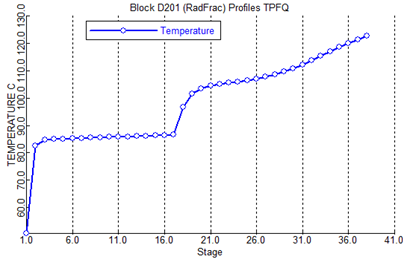
\includegraphics[scale=0.6]{example/tem.png}
	\caption{塔板温度分布图}
	\label{fig:tem}
\end{figure}

这里还有插入EPS图像和PDF图像的例子,如图\ref{fig:epspdf:a}和图\ref{fig:epspdf:b}。这里将EPS和PDF图片作为子图插入,每个子图有自己的小标题。子图标题使用subcaption宏包添加。

\begin{figure}[!htp]
  \centering
  \subcaptionbox{EPS 图像\label{fig:epspdf:a}}[3cm] %标题的长度,超过则会换行,如下一个小图。
    {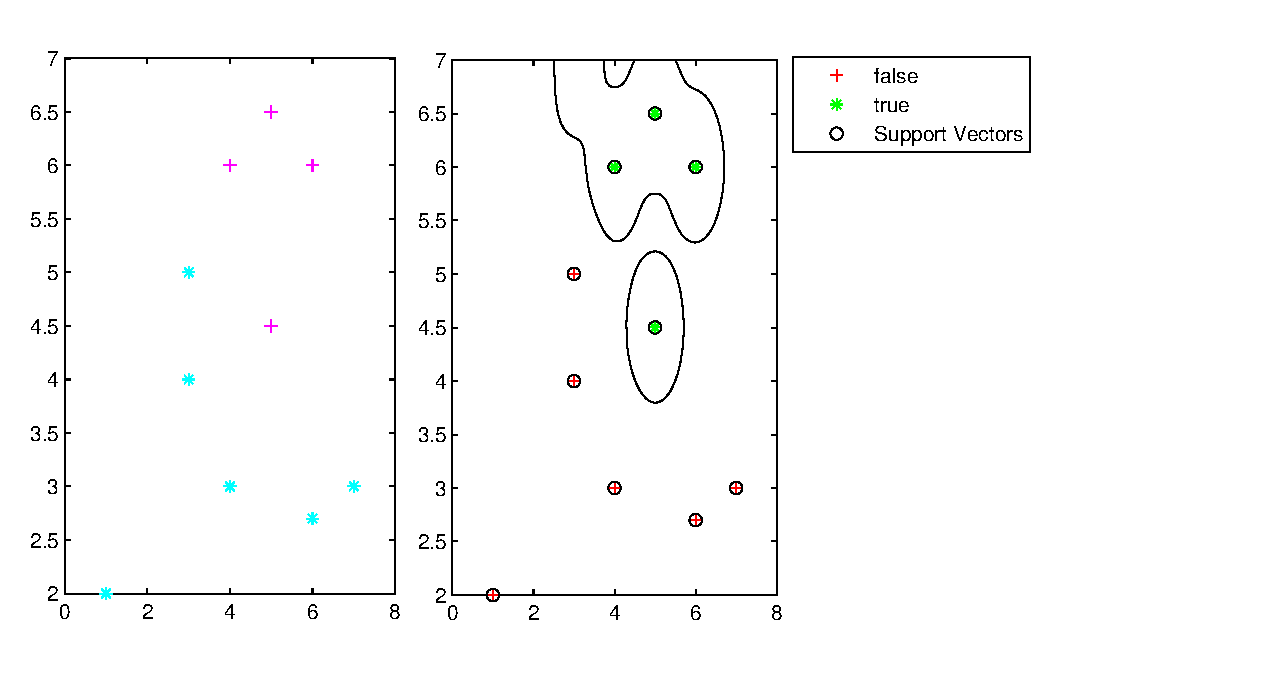
\includegraphics[height=4cm]{example/fig14.eps}}
  \hspace{4em}
  \subcaptionbox{PDF 图像。如果标题很长的话,它会自动换行\label{fig:epspdf:b}}
    {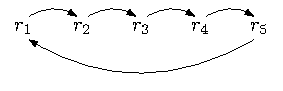
\includegraphics{example/permutation.pdf}}
  \caption{插入eps和pdf的例子(使用 subcaptionbox 方式)}
  \label{fig:pdfeps-subcaptionbox}
\end{figure}

\begin{figure}[!htp]
  \centering
  \begin{subfigure}{2.5cm}
    \centering
    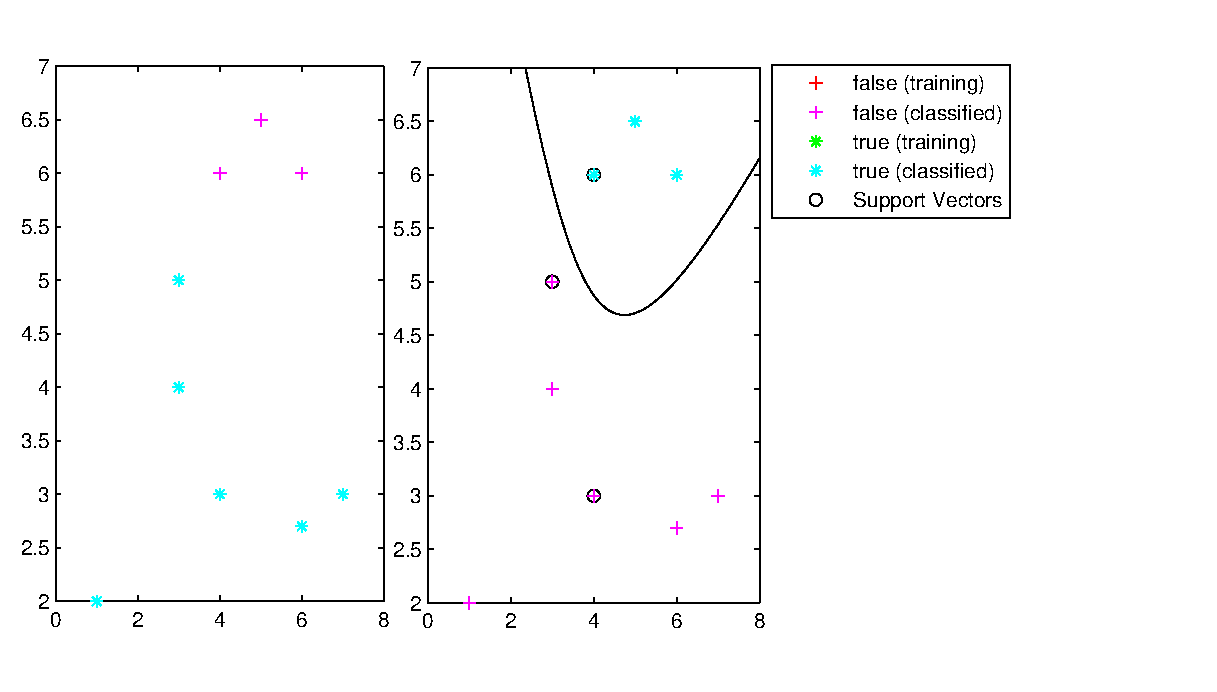
\includegraphics[height=3cm]{example/fig13.eps}
    \caption{EPS 图像}
  \end{subfigure}
  \hspace{4em}
  \begin{subfigure}{0.4\textwidth}
    \centering
    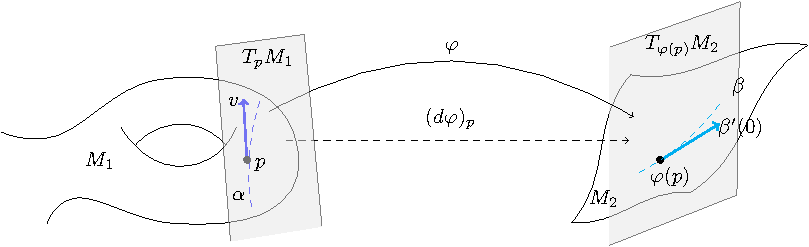
\includegraphics[height=2cm]{example/tangentmap.pdf}
    \caption{PDF 图像,注意这个图略矮些。subfigure中同一行的子图在顶端对齐。}
  \end{subfigure}
  \caption{插入eps和pdf的例子(使用 subfigure 方式)}
  \label{fig:pdfeps-subfigure}
\end{figure}

更多关于 \LaTeX 插图的例子可以参考\href{http://www.cs.duke.edu/junhu/Graphics3.pdf}{《\LaTeX 插图指南》}。

\subsection{绘制流程图}

图\ref{fig:flow_chart}是一张流程图示意。使用tikz环境,搭配四种预定义节点(\verb+startstop+、\verb+process+、\verb+decision+和\verb+io+),可以容易地绘制出流程图。
\begin{figure}[!htp]
    \centering
    \resizebox{6cm}{!}{\begin{tikzpicture}[node distance=2cm]
    \node (pic) [startstop] {待测图片};
    \node (bg) [io, below of=pic] {读取背景};
    \node (pair) [process, below of=bg] {匹配特征点对};
    \node (threshold) [decision, below of=pair, yshift=-0.5cm] {多于阈值};
    \node (clear) [decision, right of=threshold, xshift=3cm] {清晰?};
    \node (capture) [process, right of=pair, xshift=3cm, yshift=0.5cm] {重采};
    \node (matrix_p) [process, below of=threshold, yshift=-0.8cm] {透视变换矩阵};
    \node (matrix_a) [process, right of=matrix_p, xshift=3cm] {仿射变换矩阵};
    \node (reg) [process, below of=matrix_p] {图像修正};
    \node (return) [startstop, below of=reg] {配准结果};
     
    %连接具体形状
    \draw [arrow](pic) -- (bg);
    \draw [arrow](bg) -- (pair);
    \draw [arrow](pair) -- (threshold);

    \draw [arrow](threshold) -- node[anchor=south] {否} (clear);

    \draw [arrow](clear) -- node[anchor=west] {否} (capture);
    \draw [arrow](capture) |- (pic);
    \draw [arrow](clear) -- node[anchor=west] {是} (matrix_a);
    \draw [arrow](matrix_a) |- (reg);

    \draw [arrow](threshold) -- node[anchor=east] {是} (matrix_p);
    \draw [arrow](matrix_p) -- (reg);
    \draw [arrow](reg) -- (return);
\end{tikzpicture}
}
    \caption{绘制流程图效果}
    \label{fig:flow_chart}
\end{figure}

\section{表格}

这一节给出的是一些表格的例子,如表\ref{tab:firstone}所示。

\begin{table}[!hpb]
  \centering
  \caption{一个颇为标准的三线表格}
  \label{tab:firstone}
  \begin{tabular}{@{}llr@{}} \toprule
    \multicolumn{2}{c}{Item} \\ \cmidrule(r){1-2}
    Animal & Description & Price (\$)\\ \midrule
    Gnat & per gram & 13.65 \\
    & each & 0.01 \\
    Gnu & stuffed & 92.50 \\
    Emu & stuffed & 33.33 \\
    Armadillo & frozen & 8.99 \\ \bottomrule
  \end{tabular}
\end{table}

下面一个是一个更复杂的表格,用threeparttable实现带有脚注的表格,如表\ref{tab:footnote}。

\begin{table}[!htpb]
  \caption{一个带有脚注的表格的例子}
  \label{tab:footnote}
  \centering
  \begin{threeparttable}[b]
     \begin{tabular}{ccd{4}cccc}
      \toprule
      \multirow{2}{6mm}{total}&\multicolumn{2}{c}{20\tnote{1}} & \multicolumn{2}{c}{40} &  \multicolumn{2}{c}{60}\\
      \cmidrule(lr){2-3}\cmidrule(lr){4-5}\cmidrule(lr){6-7}
      &www & \multicolumn{1}{c}{k} & www & k & www & k \\ % 使用说明符 d 的列会自动进入数学模式,使用 \multicolumn 对文字表头做特殊处理
      \midrule
      &$\underset{(2.12)}{4.22}$ & 120.0140\tnote{2} & 333.15 & 0.0411 & 444.99 & 0.1387 \\
      &168.6123 & 10.86 & 255.37 & 0.0353 & 376.14 & 0.1058 \\
      &6.761    & 0.007 & 235.37 & 0.0267 & 348.66 & 0.1010 \\
      \bottomrule
    \end{tabular}
    \begin{tablenotes}
    \item [1] the first note.% or \item [a]
    \item [2] the second note.% or \item [b]
    \end{tablenotes}
  \end{threeparttable}
\end{table}

\section{参考文献管理}

 \LaTeX 具有将参考文献内容和表现形式分开管理的能力,涉及三个要素:参考文献数据库、参考文献引用格式、在正文中引用参考文献。
这样的流程需要多次编译:

\begin{enumerate}[noitemsep,topsep=0pt,parsep=0pt,partopsep=0pt]
	\item 用户将论文中需要引用的参考文献条目,录入纯文本数据库文件(bib文件)。
	\item 调用xelatex对论文模板做第一次编译,扫描文中引用的参考文献,生成参考文献入口文件(aux)文件。
	\item 调用bibtex,以参考文献格式和入口文件为输入,生成格式化以后的参考文献条目文件(bib)。
	\item 再次调用xelatex编译模板,将格式化以后的参考文献条目插入正文。
\end{enumerate}

参考文献数据库(thesis.bib)的条目,可以从Google Scholar搜索引擎\footnote{\url{https://scholar.google.com}}、CiteSeerX搜索引擎\footnote{\url{http://citeseerx.ist.psu.edu}}中查找,文献管理软件Papers\footnote{\url{http://papersapp.com}}、Mendeley\footnote{\url{http://www.mendeley.com}}、JabRef\footnote{\url{http://jabref.sourceforge.net}}也能够输出条目信息。

下面是在Google Scholar上搜索到的一条文献信息,格式是纯文本:

\begin{lstlisting}[caption={从Google Scholar找到的参考文献条目}, label=googlescholar, escapeinside="", numbers=none]
    @phdthesis{"白2008信用风险传染模型和信用衍生品的定价",
      title={"信用风险传染模型和信用衍生品的定价"},
      author={"白云芬"},
      year={2008},
      school={"上海交通大学"}
    } 
\end{lstlisting}

推荐修改后在bib文件中的内容为:

\begin{lstlisting}[caption={修改后的参考文献条目}, label=itemok, escapeinside="", numbers=none]
  @phdthesis{bai2008,
    title={"信用风险传染模型和信用衍生品的定价"},
    author={"白云芬"},
    date={2008},
    address={"上海"},
    school={"上海交通大学"}
  } 
\end{lstlisting}

按照教务处的要求,参考文献外观应符合国标GBT7714的要求\footnote{\url{http://www.cces.net.cn/guild/sites/tmxb/Files/19798_2.pdf}}。
在模板中,表现形式的控制逻辑通过biblatex-gb7714-2015包实现\footnote{\url{https://www.ctan.org/pkg/biblatex-gb7714-2015}},基于{Bib\LaTeX}管理文献。在目前的多数TeX发行版中,可能都没有默认包含biblatex-gb7714-2015,需要手动安装。

正文中引用参考文献时,用\verb+\cite{key1,key2,key3...}+可以产生“上标引用的参考文献”,
如\cite{Meta_CN,chen2007act,DPMG}。
使用\verb+\parencite{key1,key2,key3...}+则可以产生水平引用的参考文献,例如\parencite{JohnD,zhubajie,IEEE-1363}。
请看下面的例子,将会穿插使用水平的和上标的参考文献:关于书的\parencite{Meta_CN,JohnD,IEEE-1363},关于期刊的\cite{chen2007act,chen2007ewi},
会议论文\parencite{DPMG,kocher99,cnproceed},
硕士学位论文\parencite{zhubajie,metamori2004},博士学位论文\cite{shaheshang,FistSystem01,bai2008},标准文件\parencite{IEEE-1363},技术报告\cite{NPB2},电子文献\parencite{xiaoyu2001, CHRISTINE1998},用户手册\parencite{RManual}。

总结一些注意事项:
\begin{itemize}
\item 参考文献只有在正文中被引用了,才会在最后的参考文献列表中出现;
\item 参考文献“数据库文件”bib是纯文本文件,请使用UTF-8编码,不要使用GBK编码;
\item 参考文献条目中默认通过date域输入时间。兼容使用year域时会产生编译warning,可忽略。
\end{itemize}

\section{用listings插入源代码}

\begin{lstlisting}[language={C}, caption={一段C源代码}]
#include <stdio.h>
#include <unistd.h>
#include <sys/types.h>
#include <sys/wait.h>

int main() {
  pid_t pid;

  switch ((pid = fork())) {
  case -1:
    printf("fork failed\n");
    break;
  case 0:
    /* child calls exec */
    execl("/bin/ls", "ls", "-l", (char*)0);
    printf("execl failed\n");
    break;
  default:
    /* parent uses wait to suspend execution until child finishes */
    wait((int*)0);
    printf("is completed\n");
    break;
  }

  return 0;
}
\end{lstlisting}

\section{用algorithm和algorithmicx宏包插入算法描述}

algorithmicx 比 algorithmic 增加了一些命令。
示例如算法\ref{algo:sum_100}和算法\ref{algo:merge_sort},
后者的代码来自\href{http://hustsxh.is-programmer.com/posts/38801.html}{xhSong的博客}。
algorithmicx的详细使用方法见\href{http://mirror.hust.edu.cn/CTAN/macros/latex/contrib/algorithmicx/algorithmicx.pdf}{官方README}。
使用算法宏包时,算法出现的位置很多时候不按照tex文件里的书写顺序, 
需要强制定位时可以使用\verb+\begin{algorithm}[H]+
\footnote{http://tex.stackexchange.com/questions/165021/fixing-the-location-of-the-appearance-in-algorithmicx-environment}
\begin{algorithm}
% \begin{algorithm}[H] % 强制定位
\caption{求100以内的整数和}
\label{algo:sum_100}
\begin{algorithmic}[1] %每行显示行号
\Ensure 100以内的整数和 % 输出
\State $sum \gets 0$
\For{$i = 0 \to 100$}
    \State $sum \gets sum + i$
  \EndFor
\end{algorithmic}
\end{algorithm}
                         % Chapter 2
%%!TEX root = ../dissertation.tex
\begin{savequote}[75mm]
Nulla facilisi. In vel sem. Morbi id urna in diam dignissim feugiat. Proin molestie tortor eu velit. Aliquam erat volutpat. Nullam ultrices, diam tempus vulputate egestas, eros pede varius leo.
\qauthor{Quoteauthor Lastname}
\end{savequote}

\chapter{Consectetuer adipiscing elit}

\newthought{Lorem ipsum dolor sit amet}, consectetuer adipiscing elit. Morbi commodo, ipsum sed pharetra gravida, orci magna rhoncus neque, id pulvinar odio lorem non turpis. Nullam sit amet enim. Suspendisse id velit vitae ligula volutpat condimentum. Aliquam erat volutpat. Sed quis velit. Nulla facilisi. Nulla libero. Vivamus pharetra posuere sapien. Nam consectetuer. Sed aliquam, nunc eget euismod ullamcorper, lectus nunc ullamcorper orci, fermentum bibendum enim nibh eget ipsum. Donec porttitor ligula eu dolor. Maecenas vitae nulla consequat libero cursus venenatis. Nam magna enim, accumsan eu, blandit sed, blandit a, eros.

Lorem ipsum dolor sit amet, consectetuer adipiscing elit. Morbi commodo, ipsum sed pharetra gravida, orci magna rhoncus neque, id pulvinar odio lorem non turpis. Nullam sit amet enim. Suspendisse id velit vitae ligula volutpat condimentum. Aliquam erat volutpat. Sed quis velit. Nulla facilisi. Nulla libero. Vivamus pharetra posuere sapien. Nam consectetuer. Sed aliquam, nunc eget euismod ullamcorper, lectus nunc ullamcorper orci, fermentum bibendum enim nibh eget ipsum. Donec porttitor ligula eu dolor. Maecenas vitae nulla consequat libero cursus venenatis. Nam magna enim, accumsan eu, blandit sed, blandit a, eros.

Quisque facilisis erat a dui. Nam malesuada ornare dolor. Cras gravida, diam sit amet rhoncus ornare, erat elit consectetuer erat, id egestas pede nibh eget odio. Proin tincidunt, velit vel porta elementum, magna diam molestie sapien, non aliquet massa pede eu diam. Aliquam iaculis. Fusce et ipsum et nulla tristique facilisis. Donec eget sem sit amet ligula viverra gravida. Etiam vehicula urna vel turpis. Suspendisse sagittis ante a urna. Morbi a est quis orci consequat rutrum. Nullam egestas feugiat felis. Integer adipiscing semper ligula. Nunc molestie, nisl sit amet cursus convallis, sapien lectus pretium metus, vitae pretium enim wisi id lectus. Donec vestibulum. Etiam vel nibh. Nulla facilisi. Mauris pharetra. Donec augue. Fusce ultrices, neque id dignissim ultrices, tellus mauris dictum elit, vel lacinia enim metus eu nunc.

Proin at eros non eros adipiscing mollis. Donec semper turpis sed diam. Sed consequat ligula nec tortor. Integer eget sem. Ut vitae enim eu est vehicula gravida. Morbi ipsum ipsum, porta nec, tempor id, auctor vitae, purus. Pellentesque neque. Nulla luctus erat vitae libero. Integer nec enim. Phasellus aliquam enim et tortor. Quisque aliquet, quam elementum condimentum feugiat, tellus odio consectetuer wisi, vel nonummy sem neque in elit. Curabitur eleifend wisi iaculis ipsum. Pellentesque habitant morbi tristique senectus et netus et malesuada fames ac turpis egestas. In non velit non ligula laoreet ultrices. Praesent ultricies facilisis nisl. Vivamus luctus elit sit amet mi. Phasellus pellentesque, erat eget elementum volutpat, dolor nisl porta neque, vitae sodales ipsum nibh in ligula. Maecenas mattis pulvinar diam. Curabitur sed leo.

Nulla facilisi. In vel sem. Morbi id urna in diam dignissim feugiat. Proin molestie tortor eu velit. Aliquam erat volutpat. Nullam ultrices, diam tempus vulputate egestas, eros pede varius leo, sed imperdiet lectus est ornare odio. Lorem ipsum dolor sit amet, consectetuer adipiscing elit. Proin consectetuer velit in dui. Phasellus wisi purus, interdum vitae, rutrum accumsan, viverra in, velit. Sed enim risus, congue non, tristique in, commodo eu, metus. Aenean tortor mi, imperdiet id, gravida eu, posuere eu, felis. Mauris sollicitudin, turpis in hendrerit sodales, lectus ipsum pellentesque ligula, sit amet scelerisque urna nibh ut arcu. Aliquam in lacus. Vestibulum ante ipsum primis in faucibus orci luctus et ultrices posuere cubilia Curae; Nulla placerat aliquam wisi. Mauris viverra odio. Quisque fermentum pulvinar odio. Proin posuere est vitae ligula. Etiam euismod. Cras a eros.

Nunc auctor bibendum eros. Maecenas porta accumsan mauris. Etiam enim enim, elementum sed, bibendum quis, rhoncus non, metus. Fusce neque dolor, adipiscing sed, consectetuer et, lacinia sit amet, quam. Suspendisse wisi quam, consectetuer in, blandit sed, suscipit eu, eros. Etiam ligula enim, tempor ut, blandit nec, mollis eu, lectus. Nam cursus. Vivamus iaculis. Aenean risus purus, pharetra in, blandit quis, gravida a, turpis. Donec nisl. Aenean eget mi. Fusce mattis est id diam. Phasellus faucibus interdum sapien. Duis quis nunc. Sed enim.

Pellentesque vel dui sed orci faucibus iaculis. Suspendisse dictum magna id purus tincidunt rutrum. Nulla congue. Vivamus sit amet lorem posuere dui vulputate ornare. Phasellus mattis sollicitudin ligula. Duis dignissim felis et urna. Integer adipiscing congue metus. Nam pede. Etiam non wisi. Sed accumsan dolor ac augue. Pellentesque eget lectus. Aliquam nec dolor nec tellus ornare venenatis. Nullam blandit placerat sem. Curabitur quis ipsum. Mauris nisl tellus, aliquet eu, suscipit eu, ullamcorper quis, magna. Mauris elementum, pede at sodales vestibulum, nulla tortor congue massa, quis pellentesque odio dui id est. Cras faucibus augue.

Suspendisse vestibulum dignissim quam. Integer vel augue. Phasellus nulla purus, interdum ac, venenatis non, varius rutrum, leo. Pellentesque habitant morbi tristique senectus et netus et malesuada fames ac turpis egestas. Duis a eros. Class aptent taciti sociosqu ad litora torquent per conubia nostra, per inceptos hymenaeos. Fusce magna mi, porttitor quis, convallis eget, sodales ac, urna. Phasellus luctus venenatis magna. Vivamus eget lacus. Nunc tincidunt convallis tortor. Duis eros mi, dictum vel, fringilla sit amet, fermentum id, sem. Phasellus nunc enim, faucibus ut, laoreet in, consequat id, metus. Vivamus dignissim. Cras lobortis tempor velit. Phasellus nec diam ac nisl lacinia tristique. Nullam nec metus id mi dictum dignissim. Nullam quis wisi non sem lobortis condimentum. Phasellus pulvinar, nulla non aliquam eleifend, tortor wisi scelerisque felis, in sollicitudin arcu ante lacinia leo.

Pellentesque habitant morbi tristique senectus et netus et malesuada fames ac turpis egestas. Vestibulum tortor quam, feugiat vitae, ultricies eget, tempor sit amet, ante. Donec eu libero sit amet quam egestas semper. Aenean ultricies mi vitae est. Mauris placerat eleifend leo. Quisque sit amet est et sapien ullamcorper pharetra. Vestibulum erat wisi, condimentum sed, commodo vitae, ornare sit amet, wisi. Aenean fermentum, elit eget tincidunt condimentum, eros ipsum rutrum orci, sagittis tempus lacus enim ac dui. Donec non enim in turpis pulvinar facilisis. Ut felis.

Cras sed ante. Phasellus in massa. Curabitur dolor eros, gravida et, hendrerit ac, cursus non, massa. Aliquam lorem. In hac habitasse platea dictumst. Cras eu mauris. Quisque lacus. Donec ipsum. Nullam vitae sem at nunc pharetra ultricies. Vivamus elit eros, ullamcorper a, adipiscing sit amet, porttitor ut, nibh. Maecenas adipiscing mollis massa. Nunc ut dui eget nulla venenatis aliquet. Sed luctus posuere justo. Cras vehicula varius turpis. Vivamus eros metus, tristique sit amet, molestie dignissim, malesuada et, urna.

Cras dictum. Maecenas ut turpis. In vitae erat ac orci dignissim eleifend. Nunc quis justo. Sed vel ipsum in purus tincidunt pharetra. Sed pulvinar, felis id consectetuer malesuada, enim nisl mattis elit, a facilisis tortor nibh quis leo. Sed augue lacus, pretium vitae, molestie eget, rhoncus quis, elit. Donec in augue. Fusce orci wisi, ornare id, mollis vel, lacinia vel, massa.

Lorem ipsum dolor sit amet, consectetuer adipiscing elit. Morbi commodo, ipsum sed pharetra gravida, orci magna rhoncus neque, id pulvinar odio lorem non turpis. Nullam sit amet enim. Suspendisse id velit vitae ligula volutpat condimentum. Aliquam erat volutpat. Sed quis velit. Nulla facilisi. Nulla libero. Vivamus pharetra posuere sapien. Nam consectetuer. Sed aliquam, nunc eget euismod ullamcorper, lectus nunc ullamcorper orci, fermentum bibendum enim nibh eget ipsum. Donec porttitor ligula eu dolor. Maecenas vitae nulla consequat libero cursus venenatis. Nam magna enim, accumsan eu, blandit sed, blandit a, eros.

Quisque facilisis erat a dui. Nam malesuada ornare dolor. Cras gravida, diam sit amet rhoncus ornare, erat elit consectetuer erat, id egestas pede nibh eget odio. Proin tincidunt, velit vel porta elementum, magna diam molestie sapien, non aliquet massa pede eu diam. Aliquam iaculis. Fusce et ipsum et nulla tristique facilisis. Donec eget sem sit amet ligula viverra gravida. Etiam vehicula urna vel turpis. Suspendisse sagittis ante a urna. Morbi a est quis orci consequat rutrum. Nullam egestas feugiat felis. Integer adipiscing semper ligula. Nunc molestie, nisl sit amet cursus convallis, sapien lectus pretium metus, vitae pretium enim wisi id lectus. Donec vestibulum. Etiam vel nibh. Nulla facilisi. Mauris pharetra. Donec augue. Fusce ultrices, neque id dignissim ultrices, tellus mauris dictum elit, vel lacinia enim metus eu nunc.

Proin at eros non eros adipiscing mollis. Donec semper turpis sed diam. Sed consequat ligula nec tortor. Integer eget sem. Ut vitae enim eu est vehicula gravida. Morbi ipsum ipsum, porta nec, tempor id, auctor vitae, purus. Pellentesque neque. Nulla luctus erat vitae libero. Integer nec enim. Phasellus aliquam enim et tortor. Quisque aliquet, quam elementum condimentum feugiat, tellus odio consectetuer wisi, vel nonummy sem neque in elit. Curabitur eleifend wisi iaculis ipsum. Pellentesque habitant morbi tristique senectus et netus et malesuada fames ac turpis egestas. In non velit non ligula laoreet ultrices. Praesent ultricies facilisis nisl. Vivamus luctus elit sit amet mi. Phasellus pellentesque, erat eget elementum volutpat, dolor nisl porta neque, vitae sodales ipsum nibh in ligula. Maecenas mattis pulvinar diam. Curabitur sed leo.

Nulla facilisi. In vel sem. Morbi id urna in diam dignissim feugiat. Proin molestie tortor eu velit. Aliquam erat volutpat. Nullam ultrices, diam tempus vulputate egestas, eros pede varius leo, sed imperdiet lectus est ornare odio. Lorem ipsum dolor sit amet, consectetuer adipiscing elit. Proin consectetuer velit in dui. Phasellus wisi purus, interdum vitae, rutrum accumsan, viverra in, velit. Sed enim risus, congue non, tristique in, commodo eu, metus. Aenean tortor mi, imperdiet id, gravida eu, posuere eu, felis. Mauris sollicitudin, turpis in hendrerit sodales, lectus ipsum pellentesque ligula, sit amet scelerisque urna nibh ut arcu. Aliquam in lacus. Vestibulum ante ipsum primis in faucibus orci luctus et ultrices posuere cubilia Curae; Nulla placerat aliquam wisi. Mauris viverra odio. Quisque fermentum pulvinar odio. Proin posuere est vitae ligula. Etiam euismod. Cras a eros.

Nunc auctor bibendum eros. Maecenas porta accumsan mauris. Etiam enim enim, elementum sed, bibendum quis, rhoncus non, metus. Fusce neque dolor, adipiscing sed, consectetuer et, lacinia sit amet, quam. Suspendisse wisi quam, consectetuer in, blandit sed, suscipit eu, eros. Etiam ligula enim, tempor ut, blandit nec, mollis eu, lectus. Nam cursus. Vivamus iaculis. Aenean risus purus, pharetra in, blandit quis, gravida a, turpis. Donec nisl. Aenean eget mi. Fusce mattis est id diam. Phasellus faucibus interdum sapien. Duis quis nunc. Sed enim.

Pellentesque vel dui sed orci faucibus iaculis. Suspendisse dictum magna id purus tincidunt rutrum. Nulla congue. Vivamus sit amet lorem posuere dui vulputate ornare. Phasellus mattis sollicitudin ligula. Duis dignissim felis et urna. Integer adipiscing congue metus. Nam pede. Etiam non wisi. Sed accumsan dolor ac augue. Pellentesque eget lectus. Aliquam nec dolor nec tellus ornare venenatis. Nullam blandit placerat sem. Curabitur quis ipsum. Mauris nisl tellus, aliquet eu, suscipit eu, ullamcorper quis, magna. Mauris elementum, pede at sodales vestibulum, nulla tortor congue massa, quis pellentesque odio dui id est. Cras faucibus augue.

Suspendisse vestibulum dignissim quam. Integer vel augue. Phasellus nulla purus, interdum ac, venenatis non, varius rutrum, leo. Pellentesque habitant morbi tristique senectus et netus et malesuada fames ac turpis egestas. Duis a eros. Class aptent taciti sociosqu ad litora torquent per conubia nostra, per inceptos hymenaeos. Fusce magna mi, porttitor quis, convallis eget, sodales ac, urna. Phasellus luctus venenatis magna. Vivamus eget lacus. Nunc tincidunt convallis tortor. Duis eros mi, dictum vel, fringilla sit amet, fermentum id, sem. Phasellus nunc enim, faucibus ut, laoreet in, consequat id, metus. Vivamus dignissim. Cras lobortis tempor velit. Phasellus nec diam ac nisl lacinia tristique. Nullam nec metus id mi dictum dignissim. Nullam quis wisi non sem lobortis condimentum. Phasellus pulvinar, nulla non aliquam eleifend, tortor wisi scelerisque felis, in sollicitudin arcu ante lacinia leo.

Pellentesque habitant morbi tristique senectus et netus et malesuada fames ac turpis egestas. Vestibulum tortor quam, feugiat vitae, ultricies eget, tempor sit amet, ante. Donec eu libero sit amet quam egestas semper. Aenean ultricies mi vitae est. Mauris placerat eleifend leo. Quisque sit amet est et sapien ullamcorper pharetra. Vestibulum erat wisi, condimentum sed, commodo vitae, ornare sit amet, wisi. Aenean fermentum, elit eget tincidunt condimentum, eros ipsum rutrum orci, sagittis tempus lacus enim ac dui. Donec non enim in turpis pulvinar facilisis. Ut felis.

Cras sed ante. Phasellus in massa. Curabitur dolor eros, gravida et, hendrerit ac, cursus non, massa. Aliquam lorem. In hac habitasse platea dictumst. Cras eu mauris. Quisque lacus. Donec ipsum. Nullam vitae sem at nunc pharetra ultricies. Vivamus elit eros, ullamcorper a, adipiscing sit amet, porttitor ut, nibh. Maecenas adipiscing mollis massa. Nunc ut dui eget nulla venenatis aliquet. Sed luctus posuere justo. Cras vehicula varius turpis. Vivamus eros metus, tristique sit amet, molestie dignissim, malesuada et, urna.

Cras dictum. Maecenas ut turpis. In vitae erat ac orci dignissim eleifend. Nunc quis justo. Sed vel ipsum in purus tincidunt pharetra. Sed pulvinar, felis id consectetuer malesuada, enim nisl mattis elit, a facilisis tortor nibh quis leo. Sed augue lacus, pretium vitae, molestie eget, rhoncus quis, elit. Donec in augue. Fusce orci wisi, ornare id, mollis vel, lacinia vel, massa.

Lorem ipsum dolor sit amet, consectetuer adipiscing elit. Morbi commodo, ipsum sed pharetra gravida, orci magna rhoncus neque, id pulvinar odio lorem non turpis. Nullam sit amet enim. Suspendisse id velit vitae ligula volutpat condimentum. Aliquam erat volutpat. Sed quis velit. Nulla facilisi. Nulla libero. Vivamus pharetra posuere sapien. Nam consectetuer. Sed aliquam, nunc eget euismod ullamcorper, lectus nunc ullamcorper orci, fermentum bibendum enim nibh eget ipsum. Donec porttitor ligula eu dolor. Maecenas vitae nulla consequat libero cursus venenatis. Nam magna enim, accumsan eu, blandit sed, blandit a, eros.

Quisque facilisis erat a dui. Nam malesuada ornare dolor. Cras gravida, diam sit amet rhoncus ornare, erat elit consectetuer erat, id egestas pede nibh eget odio. Proin tincidunt, velit vel porta elementum, magna diam molestie sapien, non aliquet massa pede eu diam. Aliquam iaculis. Fusce et ipsum et nulla tristique facilisis. Donec eget sem sit amet ligula viverra gravida. Etiam vehicula urna vel turpis. Suspendisse sagittis ante a urna. Morbi a est quis orci consequat rutrum. Nullam egestas feugiat felis. Integer adipiscing semper ligula. Nunc molestie, nisl sit amet cursus convallis, sapien lectus pretium metus, vitae pretium enim wisi id lectus. Donec vestibulum. Etiam vel nibh. Nulla facilisi. Mauris pharetra. Donec augue. Fusce ultrices, neque id dignissim ultrices, tellus mauris dictum elit, vel lacinia enim metus eu nunc.

Proin at eros non eros adipiscing mollis. Donec semper turpis sed diam. Sed consequat ligula nec tortor. Integer eget sem. Ut vitae enim eu est vehicula gravida. Morbi ipsum ipsum, porta nec, tempor id, auctor vitae, purus. Pellentesque neque. Nulla luctus erat vitae libero. Integer nec enim. Phasellus aliquam enim et tortor. Quisque aliquet, quam elementum condimentum feugiat, tellus odio consectetuer wisi, vel nonummy sem neque in elit. Curabitur eleifend wisi iaculis ipsum. Pellentesque habitant morbi tristique senectus et netus et malesuada fames ac turpis egestas. In non velit non ligula laoreet ultrices. Praesent ultricies facilisis nisl. Vivamus luctus elit sit amet mi. Phasellus pellentesque, erat eget elementum volutpat, dolor nisl porta neque, vitae sodales ipsum nibh in ligula. Maecenas mattis pulvinar diam. Curabitur sed leo.

Nulla facilisi. In vel sem. Morbi id urna in diam dignissim feugiat. Proin molestie tortor eu velit. Aliquam erat volutpat. Nullam ultrices, diam tempus vulputate egestas, eros pede varius leo, sed imperdiet lectus est ornare odio. Lorem ipsum dolor sit amet, consectetuer adipiscing elit. Proin consectetuer velit in dui. Phasellus wisi purus, interdum vitae, rutrum accumsan, viverra in, velit. Sed enim risus, congue non, tristique in, commodo eu, metus. Aenean tortor mi, imperdiet id, gravida eu, posuere eu, felis. Mauris sollicitudin, turpis in hendrerit sodales, lectus ipsum pellentesque ligula, sit amet scelerisque urna nibh ut arcu. Aliquam in lacus. Vestibulum ante ipsum primis in faucibus orci luctus et ultrices posuere cubilia Curae; Nulla placerat aliquam wisi. Mauris viverra odio. Quisque fermentum pulvinar odio. Proin posuere est vitae ligula. Etiam euismod. Cras a eros.

Nunc auctor bibendum eros. Maecenas porta accumsan mauris. Etiam enim enim, elementum sed, bibendum quis, rhoncus non, metus. Fusce neque dolor, adipiscing sed, consectetuer et, lacinia sit amet, quam. Suspendisse wisi quam, consectetuer in, blandit sed, suscipit eu, eros. Etiam ligula enim, tempor ut, blandit nec, mollis eu, lectus. Nam cursus. Vivamus iaculis. Aenean risus purus, pharetra in, blandit quis, gravida a, turpis. Donec nisl. Aenean eget mi. Fusce mattis est id diam. Phasellus faucibus interdum sapien. Duis quis nunc. Sed enim.

Pellentesque vel dui sed orci faucibus iaculis. Suspendisse dictum magna id purus tincidunt rutrum. Nulla congue. Vivamus sit amet lorem posuere dui vulputate ornare. Phasellus mattis sollicitudin ligula. Duis dignissim felis et urna. Integer adipiscing congue metus. Nam pede. Etiam non wisi. Sed accumsan dolor ac augue. Pellentesque eget lectus. Aliquam nec dolor nec tellus ornare venenatis. Nullam blandit placerat sem. Curabitur quis ipsum. Mauris nisl tellus, aliquet eu, suscipit eu, ullamcorper quis, magna. Mauris elementum, pede at sodales vestibulum, nulla tortor congue massa, quis pellentesque odio dui id est. Cras faucibus augue.

Suspendisse vestibulum dignissim quam. Integer vel augue. Phasellus nulla purus, interdum ac, venenatis non, varius rutrum, leo. Pellentesque habitant morbi tristique senectus et netus et malesuada fames ac turpis egestas. Duis a eros. Class aptent taciti sociosqu ad litora torquent per conubia nostra, per inceptos hymenaeos. Fusce magna mi, porttitor quis, convallis eget, sodales ac, urna. Phasellus luctus venenatis magna. Vivamus eget lacus. Nunc tincidunt convallis tortor. Duis eros mi, dictum vel, fringilla sit amet, fermentum id, sem. Phasellus nunc enim, faucibus ut, laoreet in, consequat id, metus. Vivamus dignissim. Cras lobortis tempor velit. Phasellus nec diam ac nisl lacinia tristique. Nullam nec metus id mi dictum dignissim. Nullam quis wisi non sem lobortis condimentum. Phasellus pulvinar, nulla non aliquam eleifend, tortor wisi scelerisque felis, in sollicitudin arcu ante lacinia leo.

Pellentesque habitant morbi tristique senectus et netus et malesuada fames ac turpis egestas. Vestibulum tortor quam, feugiat vitae, ultricies eget, tempor sit amet, ante. Donec eu libero sit amet quam egestas semper. Aenean ultricies mi vitae est. Mauris placerat eleifend leo. Quisque sit amet est et sapien ullamcorper pharetra. Vestibulum erat wisi, condimentum sed, commodo vitae, ornare sit amet, wisi. Aenean fermentum, elit eget tincidunt condimentum, eros ipsum rutrum orci, sagittis tempus lacus enim ac dui. Donec non enim in turpis pulvinar facilisis. Ut felis.

Cras sed ante. Phasellus in massa. Curabitur dolor eros, gravida et, hendrerit ac, cursus non, massa. Aliquam lorem. In hac habitasse platea dictumst. Cras eu mauris. Quisque lacus. Donec ipsum. Nullam vitae sem at nunc pharetra ultricies. Vivamus elit eros, ullamcorper a, adipiscing sit amet, porttitor ut, nibh. Maecenas adipiscing mollis massa. Nunc ut dui eget nulla venenatis aliquet. Sed luctus posuere justo. Cras vehicula varius turpis. Vivamus eros metus, tristique sit amet, molestie dignissim, malesuada et, urna.

Cras dictum. Maecenas ut turpis. In vitae erat ac orci dignissim eleifend. Nunc quis justo. Sed vel ipsum in purus tincidunt pharetra. Sed pulvinar, felis id consectetuer malesuada, enim nisl mattis elit, a facilisis tortor nibh quis leo. Sed augue lacus, pretium vitae, molestie eget, rhoncus quis, elit. Donec in augue. Fusce orci wisi, ornare id, mollis vel, lacinia vel, massa.

Lorem ipsum dolor sit amet, consectetuer adipiscing elit. Morbi commodo, ipsum sed pharetra gravida, orci magna rhoncus neque, id pulvinar odio lorem non turpis. Nullam sit amet enim. Suspendisse id velit vitae ligula volutpat condimentum. Aliquam erat volutpat. Sed quis velit. Nulla facilisi. Nulla libero. Vivamus pharetra posuere sapien. Nam consectetuer. Sed aliquam, nunc eget euismod ullamcorper, lectus nunc ullamcorper orci, fermentum bibendum enim nibh eget ipsum. Donec porttitor ligula eu dolor. Maecenas vitae nulla consequat libero cursus venenatis. Nam magna enim, accumsan eu, blandit sed, blandit a, eros.

Quisque facilisis erat a dui. Nam malesuada ornare dolor. Cras gravida, diam sit amet rhoncus ornare, erat elit consectetuer erat, id egestas pede nibh eget odio. Proin tincidunt, velit vel porta elementum, magna diam molestie sapien, non aliquet massa pede eu diam. Aliquam iaculis. Fusce et ipsum et nulla tristique facilisis. Donec eget sem sit amet ligula viverra gravida. Etiam vehicula urna vel turpis. Suspendisse sagittis ante a urna. Morbi a est quis orci consequat rutrum. Nullam egestas feugiat felis. Integer adipiscing semper ligula. Nunc molestie, nisl sit amet cursus convallis, sapien lectus pretium metus, vitae pretium enim wisi id lectus. Donec vestibulum. Etiam vel nibh. Nulla facilisi. Mauris pharetra. Donec augue. Fusce ultrices, neque id dignissim ultrices, tellus mauris dictum elit, vel lacinia enim metus eu nunc.

Proin at eros non eros adipiscing mollis. Donec semper turpis sed diam. Sed consequat ligula nec tortor. Integer eget sem. Ut vitae enim eu est vehicula gravida. Morbi ipsum ipsum, porta nec, tempor id, auctor vitae, purus. Pellentesque neque. Nulla luctus erat vitae libero. Integer nec enim. Phasellus aliquam enim et tortor. Quisque aliquet, quam elementum condimentum feugiat, tellus odio consectetuer wisi, vel nonummy sem neque in elit. Curabitur eleifend wisi iaculis ipsum. Pellentesque habitant morbi tristique senectus et netus et malesuada fames ac turpis egestas. In non velit non ligula laoreet ultrices. Praesent ultricies facilisis nisl. Vivamus luctus elit sit amet mi. Phasellus pellentesque, erat eget elementum volutpat, dolor nisl porta neque, vitae sodales ipsum nibh in ligula. Maecenas mattis pulvinar diam. Curabitur sed leo.

Nulla facilisi. In vel sem. Morbi id urna in diam dignissim feugiat. Proin molestie tortor eu velit. Aliquam erat volutpat. Nullam ultrices, diam tempus vulputate egestas, eros pede varius leo, sed imperdiet lectus est ornare odio. Lorem ipsum dolor sit amet, consectetuer adipiscing elit. Proin consectetuer velit in dui. Phasellus wisi purus, interdum vitae, rutrum accumsan, viverra in, velit. Sed enim risus, congue non, tristique in, commodo eu, metus. Aenean tortor mi, imperdiet id, gravida eu, posuere eu, felis. Mauris sollicitudin, turpis in hendrerit sodales, lectus ipsum pellentesque ligula, sit amet scelerisque urna nibh ut arcu. Aliquam in lacus. Vestibulum ante ipsum primis in faucibus orci luctus et ultrices posuere cubilia Curae; Nulla placerat aliquam wisi. Mauris viverra odio. Quisque fermentum pulvinar odio. Proin posuere est vitae ligula. Etiam euismod. Cras a eros.

Nunc auctor bibendum eros. Maecenas porta accumsan mauris. Etiam enim enim, elementum sed, bibendum quis, rhoncus non, metus. Fusce neque dolor, adipiscing sed, consectetuer et, lacinia sit amet, quam. Suspendisse wisi quam, consectetuer in, blandit sed, suscipit eu, eros. Etiam ligula enim, tempor ut, blandit nec, mollis eu, lectus. Nam cursus. Vivamus iaculis. Aenean risus purus, pharetra in, blandit quis, gravida a, turpis. Donec nisl. Aenean eget mi. Fusce mattis est id diam. Phasellus faucibus interdum sapien. Duis quis nunc. Sed enim.

Pellentesque vel dui sed orci faucibus iaculis. Suspendisse dictum magna id purus tincidunt rutrum. Nulla congue. Vivamus sit amet lorem posuere dui vulputate ornare. Phasellus mattis sollicitudin ligula. Duis dignissim felis et urna. Integer adipiscing congue metus. Nam pede. Etiam non wisi. Sed accumsan dolor ac augue. Pellentesque eget lectus. Aliquam nec dolor nec tellus ornare venenatis. Nullam blandit placerat sem. Curabitur quis ipsum. Mauris nisl tellus, aliquet eu, suscipit eu, ullamcorper quis, magna. Mauris elementum, pede at sodales vestibulum, nulla tortor congue massa, quis pellentesque odio dui id est. Cras faucibus augue.

Suspendisse vestibulum dignissim quam. Integer vel augue. Phasellus nulla purus, interdum ac, venenatis non, varius rutrum, leo. Pellentesque habitant morbi tristique senectus et netus et malesuada fames ac turpis egestas. Duis a eros. Class aptent taciti sociosqu ad litora torquent per conubia nostra, per inceptos hymenaeos. Fusce magna mi, porttitor quis, convallis eget, sodales ac, urna. Phasellus luctus venenatis magna. Vivamus eget lacus. Nunc tincidunt convallis tortor. Duis eros mi, dictum vel, fringilla sit amet, fermentum id, sem. Phasellus nunc enim, faucibus ut, laoreet in, consequat id, metus. Vivamus dignissim. Cras lobortis tempor velit. Phasellus nec diam ac nisl lacinia tristique. Nullam nec metus id mi dictum dignissim. Nullam quis wisi non sem lobortis condimentum. Phasellus pulvinar, nulla non aliquam eleifend, tortor wisi scelerisque felis, in sollicitudin arcu ante lacinia leo.

Pellentesque habitant morbi tristique senectus et netus et malesuada fames ac turpis egestas. Vestibulum tortor quam, feugiat vitae, ultricies eget, tempor sit amet, ante. Donec eu libero sit amet quam egestas semper. Aenean ultricies mi vitae est. Mauris placerat eleifend leo. Quisque sit amet est et sapien ullamcorper pharetra. Vestibulum erat wisi, condimentum sed, commodo vitae, ornare sit amet, wisi. Aenean fermentum, elit eget tincidunt condimentum, eros ipsum rutrum orci, sagittis tempus lacus enim ac dui. Donec non enim in turpis pulvinar facilisis. Ut felis.

Cras sed ante. Phasellus in massa. Curabitur dolor eros, gravida et, hendrerit ac, cursus non, massa. Aliquam lorem. In hac habitasse platea dictumst. Cras eu mauris. Quisque lacus. Donec ipsum. Nullam vitae sem at nunc pharetra ultricies. Vivamus elit eros, ullamcorper a, adipiscing sit amet, porttitor ut, nibh. Maecenas adipiscing mollis massa. Nunc ut dui eget nulla venenatis aliquet. Sed luctus posuere justo. Cras vehicula varius turpis. Vivamus eros metus, tristique sit amet, molestie dignissim, malesuada et, urna.

Cras dictum. Maecenas ut turpis. In vitae erat ac orci dignissim eleifend. Nunc quis justo. Sed vel ipsum in purus tincidunt pharetra. Sed pulvinar, felis id consectetuer malesuada, enim nisl mattis elit, a facilisis tortor nibh quis leo. Sed augue lacus, pretium vitae, molestie eget, rhoncus quis, elit. Donec in augue. Fusce orci wisi, ornare id, mollis vel, lacinia vel, massa.

Lorem ipsum dolor sit amet, consectetuer adipiscing elit. Morbi commodo, ipsum sed pharetra gravida, orci magna rhoncus neque, id pulvinar odio lorem non turpis. Nullam sit amet enim. Suspendisse id velit vitae ligula volutpat condimentum. Aliquam erat volutpat. Sed quis velit. Nulla facilisi. Nulla libero. Vivamus pharetra posuere sapien. Nam consectetuer. Sed aliquam, nunc eget euismod ullamcorper, lectus nunc ullamcorper orci, fermentum bibendum enim nibh eget ipsum. Donec porttitor ligula eu dolor. Maecenas vitae nulla consequat libero cursus venenatis. Nam magna enim, accumsan eu, blandit sed, blandit a, eros.

Quisque facilisis erat a dui. Nam malesuada ornare dolor. Cras gravida, diam sit amet rhoncus ornare, erat elit consectetuer erat, id egestas pede nibh eget odio. Proin tincidunt, velit vel porta elementum, magna diam molestie sapien, non aliquet massa pede eu diam. Aliquam iaculis. Fusce et ipsum et nulla tristique facilisis. Donec eget sem sit amet ligula viverra gravida. Etiam vehicula urna vel turpis. Suspendisse sagittis ante a urna. Morbi a est quis orci consequat rutrum. Nullam egestas feugiat felis. Integer adipiscing semper ligula. Nunc molestie, nisl sit amet cursus convallis, sapien lectus pretium metus, vitae pretium enim wisi id lectus. Donec vestibulum. Etiam vel nibh. Nulla facilisi. Mauris pharetra. Donec augue. Fusce ultrices, neque id dignissim ultrices, tellus mauris dictum elit, vel lacinia enim metus eu nunc.

Proin at eros non eros adipiscing mollis. Donec semper turpis sed diam. Sed consequat ligula nec tortor. Integer eget sem. Ut vitae enim eu est vehicula gravida. Morbi ipsum ipsum, porta nec, tempor id, auctor vitae, purus. Pellentesque neque. Nulla luctus erat vitae libero. Integer nec enim. Phasellus aliquam enim et tortor. Quisque aliquet, quam elementum condimentum feugiat, tellus odio consectetuer wisi, vel nonummy sem neque in elit. Curabitur eleifend wisi iaculis ipsum. Pellentesque habitant morbi tristique senectus et netus et malesuada fames ac turpis egestas. In non velit non ligula laoreet ultrices. Praesent ultricies facilisis nisl. Vivamus luctus elit sit amet mi. Phasellus pellentesque, erat eget elementum volutpat, dolor nisl porta neque, vitae sodales ipsum nibh in ligula. Maecenas mattis pulvinar diam. Curabitur sed leo.

Nulla facilisi. In vel sem. Morbi id urna in diam dignissim feugiat. Proin molestie tortor eu velit. Aliquam erat volutpat. Nullam ultrices, diam tempus vulputate egestas, eros pede varius leo, sed imperdiet lectus est ornare odio. Lorem ipsum dolor sit amet, consectetuer adipiscing elit. Proin consectetuer velit in dui. Phasellus wisi purus, interdum vitae, rutrum accumsan, viverra in, velit. Sed enim risus, congue non, tristique in, commodo eu, metus. Aenean tortor mi, imperdiet id, gravida eu, posuere eu, felis. Mauris sollicitudin, turpis in hendrerit sodales, lectus ipsum pellentesque ligula, sit amet scelerisque urna nibh ut arcu. Aliquam in lacus. Vestibulum ante ipsum primis in faucibus orci luctus et ultrices posuere cubilia Curae; Nulla placerat aliquam wisi. Mauris viverra odio. Quisque fermentum pulvinar odio. Proin posuere est vitae ligula. Etiam euismod. Cras a eros.

Nunc auctor bibendum eros. Maecenas porta accumsan mauris. Etiam enim enim, elementum sed, bibendum quis, rhoncus non, metus. Fusce neque dolor, adipiscing sed, consectetuer et, lacinia sit amet, quam. Suspendisse wisi quam, consectetuer in, blandit sed, suscipit eu, eros. Etiam ligula enim, tempor ut, blandit nec, mollis eu, lectus. Nam cursus. Vivamus iaculis. Aenean risus purus, pharetra in, blandit quis, gravida a, turpis. Donec nisl. Aenean eget mi. Fusce mattis est id diam. Phasellus faucibus interdum sapien. Duis quis nunc. Sed enim.

Pellentesque vel dui sed orci faucibus iaculis. Suspendisse dictum magna id purus tincidunt rutrum. Nulla congue. Vivamus sit amet lorem posuere dui vulputate ornare. Phasellus mattis sollicitudin ligula. Duis dignissim felis et urna. Integer adipiscing congue metus. Nam pede. Etiam non wisi. Sed accumsan dolor ac augue. Pellentesque eget lectus. Aliquam nec dolor nec tellus ornare venenatis. Nullam blandit placerat sem. Curabitur quis ipsum. Mauris nisl tellus, aliquet eu, suscipit eu, ullamcorper quis, magna. Mauris elementum, pede at sodales vestibulum, nulla tortor congue massa, quis pellentesque odio dui id est. Cras faucibus augue.

Suspendisse vestibulum dignissim quam. Integer vel augue. Phasellus nulla purus, interdum ac, venenatis non, varius rutrum, leo. Pellentesque habitant morbi tristique senectus et netus et malesuada fames ac turpis egestas. Duis a eros. Class aptent taciti sociosqu ad litora torquent per conubia nostra, per inceptos hymenaeos. Fusce magna mi, porttitor quis, convallis eget, sodales ac, urna. Phasellus luctus venenatis magna. Vivamus eget lacus. Nunc tincidunt convallis tortor. Duis eros mi, dictum vel, fringilla sit amet, fermentum id, sem. Phasellus nunc enim, faucibus ut, laoreet in, consequat id, metus. Vivamus dignissim. Cras lobortis tempor velit. Phasellus nec diam ac nisl lacinia tristique. Nullam nec metus id mi dictum dignissim. Nullam quis wisi non sem lobortis condimentum. Phasellus pulvinar, nulla non aliquam eleifend, tortor wisi scelerisque felis, in sollicitudin arcu ante lacinia leo.

Pellentesque habitant morbi tristique senectus et netus et malesuada fames ac turpis egestas. Vestibulum tortor quam, feugiat vitae, ultricies eget, tempor sit amet, ante. Donec eu libero sit amet quam egestas semper. Aenean ultricies mi vitae est. Mauris placerat eleifend leo. Quisque sit amet est et sapien ullamcorper pharetra. Vestibulum erat wisi, condimentum sed, commodo vitae, ornare sit amet, wisi. Aenean fermentum, elit eget tincidunt condimentum, eros ipsum rutrum orci, sagittis tempus lacus enim ac dui. Donec non enim in turpis pulvinar facilisis. Ut felis.

Cras sed ante. Phasellus in massa. Curabitur dolor eros, gravida et, hendrerit ac, cursus non, massa. Aliquam lorem. In hac habitasse platea dictumst. Cras eu mauris. Quisque lacus. Donec ipsum. Nullam vitae sem at nunc pharetra ultricies. Vivamus elit eros, ullamcorper a, adipiscing sit amet, porttitor ut, nibh. Maecenas adipiscing mollis massa. Nunc ut dui eget nulla venenatis aliquet. Sed luctus posuere justo. Cras vehicula varius turpis. Vivamus eros metus, tristique sit amet, molestie dignissim, malesuada et, urna.

Cras dictum. Maecenas ut turpis. In vitae erat ac orci dignissim eleifend. Nunc quis justo. Sed vel ipsum in purus tincidunt pharetra. Sed pulvinar, felis id consectetuer malesuada, enim nisl mattis elit, a facilisis tortor nibh quis leo. Sed augue lacus, pretium vitae, molestie eget, rhoncus quis, elit. Donec in augue. Fusce orci wisi, ornare id, mollis vel, lacinia vel, massa.

Lorem ipsum dolor sit amet, consectetuer adipiscing elit. Morbi commodo, ipsum sed pharetra gravida, orci magna rhoncus neque, id pulvinar odio lorem non turpis. Nullam sit amet enim. Suspendisse id velit vitae ligula volutpat condimentum. Aliquam erat volutpat. Sed quis velit. Nulla facilisi. Nulla libero. Vivamus pharetra posuere sapien. Nam consectetuer. Sed aliquam, nunc eget euismod ullamcorper, lectus nunc ullamcorper orci, fermentum bibendum enim nibh eget ipsum. Donec porttitor ligula eu dolor. Maecenas vitae nulla consequat libero cursus venenatis. Nam magna enim, accumsan eu, blandit sed, blandit a, eros.

Quisque facilisis erat a dui. Nam malesuada ornare dolor. Cras gravida, diam sit amet rhoncus ornare, erat elit consectetuer erat, id egestas pede nibh eget odio. Proin tincidunt, velit vel porta elementum, magna diam molestie sapien, non aliquet massa pede eu diam. Aliquam iaculis. Fusce et ipsum et nulla tristique facilisis. Donec eget sem sit amet ligula viverra gravida. Etiam vehicula urna vel turpis. Suspendisse sagittis ante a urna. Morbi a est quis orci consequat rutrum. Nullam egestas feugiat felis. Integer adipiscing semper ligula. Nunc molestie, nisl sit amet cursus convallis, sapien lectus pretium metus, vitae pretium enim wisi id lectus. Donec vestibulum. Etiam vel nibh. Nulla facilisi. Mauris pharetra. Donec augue. Fusce ultrices, neque id dignissim ultrices, tellus mauris dictum elit, vel lacinia enim metus eu nunc.

Proin at eros non eros adipiscing mollis. Donec semper turpis sed diam. Sed consequat ligula nec tortor. Integer eget sem. Ut vitae enim eu est vehicula gravida. Morbi ipsum ipsum, porta nec, tempor id, auctor vitae, purus. Pellentesque neque. Nulla luctus erat vitae libero. Integer nec enim. Phasellus aliquam enim et tortor. Quisque aliquet, quam elementum condimentum feugiat, tellus odio consectetuer wisi, vel nonummy sem neque in elit. Curabitur eleifend wisi iaculis ipsum. Pellentesque habitant morbi tristique senectus et netus et malesuada fames ac turpis egestas. In non velit non ligula laoreet ultrices. Praesent ultricies facilisis nisl. Vivamus luctus elit sit amet mi. Phasellus pellentesque, erat eget elementum volutpat, dolor nisl porta neque, vitae sodales ipsum nibh in ligula. Maecenas mattis pulvinar diam. Curabitur sed leo.

Nulla facilisi. In vel sem. Morbi id urna in diam dignissim feugiat. Proin molestie tortor eu velit. Aliquam erat volutpat. Nullam ultrices, diam tempus vulputate egestas, eros pede varius leo, sed imperdiet lectus est ornare odio. Lorem ipsum dolor sit amet, consectetuer adipiscing elit. Proin consectetuer velit in dui. Phasellus wisi purus, interdum vitae, rutrum accumsan, viverra in, velit. Sed enim risus, congue non, tristique in, commodo eu, metus. Aenean tortor mi, imperdiet id, gravida eu, posuere eu, felis. Mauris sollicitudin, turpis in hendrerit sodales, lectus ipsum pellentesque ligula, sit amet scelerisque urna nibh ut arcu. Aliquam in lacus. Vestibulum ante ipsum primis in faucibus orci luctus et ultrices posuere cubilia Curae; Nulla placerat aliquam wisi. Mauris viverra odio. Quisque fermentum pulvinar odio. Proin posuere est vitae ligula. Etiam euismod. Cras a eros.

Nunc auctor bibendum eros. Maecenas porta accumsan mauris. Etiam enim enim, elementum sed, bibendum quis, rhoncus non, metus. Fusce neque dolor, adipiscing sed, consectetuer et, lacinia sit amet, quam. Suspendisse wisi quam, consectetuer in, blandit sed, suscipit eu, eros. Etiam ligula enim, tempor ut, blandit nec, mollis eu, lectus. Nam cursus. Vivamus iaculis. Aenean risus purus, pharetra in, blandit quis, gravida a, turpis. Donec nisl. Aenean eget mi. Fusce mattis est id diam. Phasellus faucibus interdum sapien. Duis quis nunc. Sed enim.

Pellentesque vel dui sed orci faucibus iaculis. Suspendisse dictum magna id purus tincidunt rutrum. Nulla congue. Vivamus sit amet lorem posuere dui vulputate ornare. Phasellus mattis sollicitudin ligula. Duis dignissim felis et urna. Integer adipiscing congue metus. Nam pede. Etiam non wisi. Sed accumsan dolor ac augue. Pellentesque eget lectus. Aliquam nec dolor nec tellus ornare venenatis. Nullam blandit placerat sem. Curabitur quis ipsum. Mauris nisl tellus, aliquet eu, suscipit eu, ullamcorper quis, magna. Mauris elementum, pede at sodales vestibulum, nulla tortor congue massa, quis pellentesque odio dui id est. Cras faucibus augue.

Suspendisse vestibulum dignissim quam. Integer vel augue. Phasellus nulla purus, interdum ac, venenatis non, varius rutrum, leo. Pellentesque habitant morbi tristique senectus et netus et malesuada fames ac turpis egestas. Duis a eros. Class aptent taciti sociosqu ad litora torquent per conubia nostra, per inceptos hymenaeos. Fusce magna mi, porttitor quis, convallis eget, sodales ac, urna. Phasellus luctus venenatis magna. Vivamus eget lacus. Nunc tincidunt convallis tortor. Duis eros mi, dictum vel, fringilla sit amet, fermentum id, sem. Phasellus nunc enim, faucibus ut, laoreet in, consequat id, metus. Vivamus dignissim. Cras lobortis tempor velit. Phasellus nec diam ac nisl lacinia tristique. Nullam nec metus id mi dictum dignissim. Nullam quis wisi non sem lobortis condimentum. Phasellus pulvinar, nulla non aliquam eleifend, tortor wisi scelerisque felis, in sollicitudin arcu ante lacinia leo.

Pellentesque habitant morbi tristique senectus et netus et malesuada fames ac turpis egestas. Vestibulum tortor quam, feugiat vitae, ultricies eget, tempor sit amet, ante. Donec eu libero sit amet quam egestas semper. Aenean ultricies mi vitae est. Mauris placerat eleifend leo. Quisque sit amet est et sapien ullamcorper pharetra. Vestibulum erat wisi, condimentum sed, commodo vitae, ornare sit amet, wisi. Aenean fermentum, elit eget tincidunt condimentum, eros ipsum rutrum orci, sagittis tempus lacus enim ac dui. Donec non enim in turpis pulvinar facilisis. Ut felis.

Cras sed ante. Phasellus in massa. Curabitur dolor eros, gravida et, hendrerit ac, cursus non, massa. Aliquam lorem. In hac habitasse platea dictumst. Cras eu mauris. Quisque lacus. Donec ipsum. Nullam vitae sem at nunc pharetra ultricies. Vivamus elit eros, ullamcorper a, adipiscing sit amet, porttitor ut, nibh. Maecenas adipiscing mollis massa. Nunc ut dui eget nulla venenatis aliquet. Sed luctus posuere justo. Cras vehicula varius turpis. Vivamus eros metus, tristique sit amet, molestie dignissim, malesuada et, urna.

Cras dictum. Maecenas ut turpis. In vitae erat ac orci dignissim eleifend. Nunc quis justo. Sed vel ipsum in purus tincidunt pharetra. Sed pulvinar, felis id consectetuer malesuada, enim nisl mattis elit, a facilisis tortor nibh quis leo. Sed augue lacus, pretium vitae, molestie eget, rhoncus quis, elit. Donec in augue. Fusce orci wisi, ornare id, mollis vel, lacinia vel, massa.

Lorem ipsum dolor sit amet, consectetuer adipiscing elit. Morbi commodo, ipsum sed pharetra gravida, orci magna rhoncus neque, id pulvinar odio lorem non turpis. Nullam sit amet enim. Suspendisse id velit vitae ligula volutpat condimentum. Aliquam erat volutpat. Sed quis velit. Nulla facilisi. Nulla libero. Vivamus pharetra posuere sapien. Nam consectetuer. Sed aliquam, nunc eget euismod ullamcorper, lectus nunc ullamcorper orci, fermentum bibendum enim nibh eget ipsum. Donec porttitor ligula eu dolor. Maecenas vitae nulla consequat libero cursus venenatis. Nam magna enim, accumsan eu, blandit sed, blandit a, eros.

Quisque facilisis erat a dui. Nam malesuada ornare dolor. Cras gravida, diam sit amet rhoncus ornare, erat elit consectetuer erat, id egestas pede nibh eget odio. Proin tincidunt, velit vel porta elementum, magna diam molestie sapien, non aliquet massa pede eu diam. Aliquam iaculis. Fusce et ipsum et nulla tristique facilisis. Donec eget sem sit amet ligula viverra gravida. Etiam vehicula urna vel turpis. Suspendisse sagittis ante a urna. Morbi a est quis orci consequat rutrum. Nullam egestas feugiat felis. Integer adipiscing semper ligula. Nunc molestie, nisl sit amet cursus convallis, sapien lectus pretium metus, vitae pretium enim wisi id lectus. Donec vestibulum. Etiam vel nibh. Nulla facilisi. Mauris pharetra. Donec augue. Fusce ultrices, neque id dignissim ultrices, tellus mauris dictum elit, vel lacinia enim metus eu nunc.

Proin at eros non eros adipiscing mollis. Donec semper turpis sed diam. Sed consequat ligula nec tortor. Integer eget sem. Ut vitae enim eu est vehicula gravida. Morbi ipsum ipsum, porta nec, tempor id, auctor vitae, purus. Pellentesque neque. Nulla luctus erat vitae libero. Integer nec enim. Phasellus aliquam enim et tortor. Quisque aliquet, quam elementum condimentum feugiat, tellus odio consectetuer wisi, vel nonummy sem neque in elit. Curabitur eleifend wisi iaculis ipsum. Pellentesque habitant morbi tristique senectus et netus et malesuada fames ac turpis egestas. In non velit non ligula laoreet ultrices. Praesent ultricies facilisis nisl. Vivamus luctus elit sit amet mi. Phasellus pellentesque, erat eget elementum volutpat, dolor nisl porta neque, vitae sodales ipsum nibh in ligula. Maecenas mattis pulvinar diam. Curabitur sed leo.

Nulla facilisi. In vel sem. Morbi id urna in diam dignissim feugiat. Proin molestie tortor eu velit. Aliquam erat volutpat. Nullam ultrices, diam tempus vulputate egestas, eros pede varius leo, sed imperdiet lectus est ornare odio. Lorem ipsum dolor sit amet, consectetuer adipiscing elit. Proin consectetuer velit in dui. Phasellus wisi purus, interdum vitae, rutrum accumsan, viverra in, velit. Sed enim risus, congue non, tristique in, commodo eu, metus. Aenean tortor mi, imperdiet id, gravida eu, posuere eu, felis. Mauris sollicitudin, turpis in hendrerit sodales, lectus ipsum pellentesque ligula, sit amet scelerisque urna nibh ut arcu. Aliquam in lacus. Vestibulum ante ipsum primis in faucibus orci luctus et ultrices posuere cubilia Curae; Nulla placerat aliquam wisi. Mauris viverra odio. Quisque fermentum pulvinar odio. Proin posuere est vitae ligula. Etiam euismod. Cras a eros.

Nunc auctor bibendum eros. Maecenas porta accumsan mauris. Etiam enim enim, elementum sed, bibendum quis, rhoncus non, metus. Fusce neque dolor, adipiscing sed, consectetuer et, lacinia sit amet, quam. Suspendisse wisi quam, consectetuer in, blandit sed, suscipit eu, eros. Etiam ligula enim, tempor ut, blandit nec, mollis eu, lectus. Nam cursus. Vivamus iaculis. Aenean risus purus, pharetra in, blandit quis, gravida a, turpis. Donec nisl. Aenean eget mi. Fusce mattis est id diam. Phasellus faucibus interdum sapien. Duis quis nunc. Sed enim.

Pellentesque vel dui sed orci faucibus iaculis. Suspendisse dictum magna id purus tincidunt rutrum. Nulla congue. Vivamus sit amet lorem posuere dui vulputate ornare. Phasellus mattis sollicitudin ligula. Duis dignissim felis et urna. Integer adipiscing congue metus. Nam pede. Etiam non wisi. Sed accumsan dolor ac augue. Pellentesque eget lectus. Aliquam nec dolor nec tellus ornare venenatis. Nullam blandit placerat sem. Curabitur quis ipsum. Mauris nisl tellus, aliquet eu, suscipit eu, ullamcorper quis, magna. Mauris elementum, pede at sodales vestibulum, nulla tortor congue massa, quis pellentesque odio dui id est. Cras faucibus augue.

Suspendisse vestibulum dignissim quam. Integer vel augue. Phasellus nulla purus, interdum ac, venenatis non, varius rutrum, leo. Pellentesque habitant morbi tristique senectus et netus et malesuada fames ac turpis egestas. Duis a eros. Class aptent taciti sociosqu ad litora torquent per conubia nostra, per inceptos hymenaeos. Fusce magna mi, porttitor quis, convallis eget, sodales ac, urna. Phasellus luctus venenatis magna. Vivamus eget lacus. Nunc tincidunt convallis tortor. Duis eros mi, dictum vel, fringilla sit amet, fermentum id, sem. Phasellus nunc enim, faucibus ut, laoreet in, consequat id, metus. Vivamus dignissim. Cras lobortis tempor velit. Phasellus nec diam ac nisl lacinia tristique. Nullam nec metus id mi dictum dignissim. Nullam quis wisi non sem lobortis condimentum. Phasellus pulvinar, nulla non aliquam eleifend, tortor wisi scelerisque felis, in sollicitudin arcu ante lacinia leo.

Pellentesque habitant morbi tristique senectus et netus et malesuada fames ac turpis egestas. Vestibulum tortor quam, feugiat vitae, ultricies eget, tempor sit amet, ante. Donec eu libero sit amet quam egestas semper. Aenean ultricies mi vitae est. Mauris placerat eleifend leo. Quisque sit amet est et sapien ullamcorper pharetra. Vestibulum erat wisi, condimentum sed, commodo vitae, ornare sit amet, wisi. Aenean fermentum, elit eget tincidunt condimentum, eros ipsum rutrum orci, sagittis tempus lacus enim ac dui. Donec non enim in turpis pulvinar facilisis. Ut felis.

Cras sed ante. Phasellus in massa. Curabitur dolor eros, gravida et, hendrerit ac, cursus non, massa. Aliquam lorem. In hac habitasse platea dictumst. Cras eu mauris. Quisque lacus. Donec ipsum. Nullam vitae sem at nunc pharetra ultricies. Vivamus elit eros, ullamcorper a, adipiscing sit amet, porttitor ut, nibh. Maecenas adipiscing mollis massa. Nunc ut dui eget nulla venenatis aliquet. Sed luctus posuere justo. Cras vehicula varius turpis. Vivamus eros metus, tristique sit amet, molestie dignissim, malesuada et, urna.

Cras dictum. Maecenas ut turpis. In vitae erat ac orci dignissim eleifend. Nunc quis justo. Sed vel ipsum in purus tincidunt pharetra. Sed pulvinar, felis id consectetuer malesuada, enim nisl mattis elit, a facilisis tortor nibh quis leo. Sed augue lacus, pretium vitae, molestie eget, rhoncus quis, elit. Donec in augue. Fusce orci wisi, ornare id, mollis vel, lacinia vel, massa.

Lorem ipsum dolor sit amet, consectetuer adipiscing elit. Morbi commodo, ipsum sed pharetra gravida, orci magna rhoncus neque, id pulvinar odio lorem non turpis. Nullam sit amet enim. Suspendisse id velit vitae ligula volutpat condimentum. Aliquam erat volutpat. Sed quis velit. Nulla facilisi. Nulla libero. Vivamus pharetra posuere sapien. Nam consectetuer. Sed aliquam, nunc eget euismod ullamcorper, lectus nunc ullamcorper orci, fermentum bibendum enim nibh eget ipsum. Donec porttitor ligula eu dolor. Maecenas vitae nulla consequat libero cursus venenatis. Nam magna enim, accumsan eu, blandit sed, blandit a, eros.

Quisque facilisis erat a dui. Nam malesuada ornare dolor. Cras gravida, diam sit amet rhoncus ornare, erat elit consectetuer erat, id egestas pede nibh eget odio. Proin tincidunt, velit vel porta elementum, magna diam molestie sapien, non aliquet massa pede eu diam. Aliquam iaculis. Fusce et ipsum et nulla tristique facilisis. Donec eget sem sit amet ligula viverra gravida. Etiam vehicula urna vel turpis. Suspendisse sagittis ante a urna. Morbi a est quis orci consequat rutrum. Nullam egestas feugiat felis. Integer adipiscing semper ligula. Nunc molestie, nisl sit amet cursus convallis, sapien lectus pretium metus, vitae pretium enim wisi id lectus. Donec vestibulum. Etiam vel nibh. Nulla facilisi. Mauris pharetra. Donec augue. Fusce ultrices, neque id dignissim ultrices, tellus mauris dictum elit, vel lacinia enim metus eu nunc.

Proin at eros non eros adipiscing mollis. Donec semper turpis sed diam. Sed consequat ligula nec tortor. Integer eget sem. Ut vitae enim eu est vehicula gravida. Morbi ipsum ipsum, porta nec, tempor id, auctor vitae, purus. Pellentesque neque. Nulla luctus erat vitae libero. Integer nec enim. Phasellus aliquam enim et tortor. Quisque aliquet, quam elementum condimentum feugiat, tellus odio consectetuer wisi, vel nonummy sem neque in elit. Curabitur eleifend wisi iaculis ipsum. Pellentesque habitant morbi tristique senectus et netus et malesuada fames ac turpis egestas. In non velit non ligula laoreet ultrices. Praesent ultricies facilisis nisl. Vivamus luctus elit sit amet mi. Phasellus pellentesque, erat eget elementum volutpat, dolor nisl porta neque, vitae sodales ipsum nibh in ligula. Maecenas mattis pulvinar diam. Curabitur sed leo.

Nulla facilisi. In vel sem. Morbi id urna in diam dignissim feugiat. Proin molestie tortor eu velit. Aliquam erat volutpat. Nullam ultrices, diam tempus vulputate egestas, eros pede varius leo, sed imperdiet lectus est ornare odio. Lorem ipsum dolor sit amet, consectetuer adipiscing elit. Proin consectetuer velit in dui. Phasellus wisi purus, interdum vitae, rutrum accumsan, viverra in, velit. Sed enim risus, congue non, tristique in, commodo eu, metus. Aenean tortor mi, imperdiet id, gravida eu, posuere eu, felis. Mauris sollicitudin, turpis in hendrerit sodales, lectus ipsum pellentesque ligula, sit amet scelerisque urna nibh ut arcu. Aliquam in lacus. Vestibulum ante ipsum primis in faucibus orci luctus et ultrices posuere cubilia Curae; Nulla placerat aliquam wisi. Mauris viverra odio. Quisque fermentum pulvinar odio. Proin posuere est vitae ligula. Etiam euismod. Cras a eros.

Nunc auctor bibendum eros. Maecenas porta accumsan mauris. Etiam enim enim, elementum sed, bibendum quis, rhoncus non, metus. Fusce neque dolor, adipiscing sed, consectetuer et, lacinia sit amet, quam. Suspendisse wisi quam, consectetuer in, blandit sed, suscipit eu, eros. Etiam ligula enim, tempor ut, blandit nec, mollis eu, lectus. Nam cursus. Vivamus iaculis. Aenean risus purus, pharetra in, blandit quis, gravida a, turpis. Donec nisl. Aenean eget mi. Fusce mattis est id diam. Phasellus faucibus interdum sapien. Duis quis nunc. Sed enim.

Pellentesque vel dui sed orci faucibus iaculis. Suspendisse dictum magna id purus tincidunt rutrum. Nulla congue. Vivamus sit amet lorem posuere dui vulputate ornare. Phasellus mattis sollicitudin ligula. Duis dignissim felis et urna. Integer adipiscing congue metus. Nam pede. Etiam non wisi. Sed accumsan dolor ac augue. Pellentesque eget lectus. Aliquam nec dolor nec tellus ornare venenatis. Nullam blandit placerat sem. Curabitur quis ipsum. Mauris nisl tellus, aliquet eu, suscipit eu, ullamcorper quis, magna. Mauris elementum, pede at sodales vestibulum, nulla tortor congue massa, quis pellentesque odio dui id est. Cras faucibus augue.

Suspendisse vestibulum dignissim quam. Integer vel augue. Phasellus nulla purus, interdum ac, venenatis non, varius rutrum, leo. Pellentesque habitant morbi tristique senectus et netus et malesuada fames ac turpis egestas. Duis a eros. Class aptent taciti sociosqu ad litora torquent per conubia nostra, per inceptos hymenaeos. Fusce magna mi, porttitor quis, convallis eget, sodales ac, urna. Phasellus luctus venenatis magna. Vivamus eget lacus. Nunc tincidunt convallis tortor. Duis eros mi, dictum vel, fringilla sit amet, fermentum id, sem. Phasellus nunc enim, faucibus ut, laoreet in, consequat id, metus. Vivamus dignissim. Cras lobortis tempor velit. Phasellus nec diam ac nisl lacinia tristique. Nullam nec metus id mi dictum dignissim. Nullam quis wisi non sem lobortis condimentum. Phasellus pulvinar, nulla non aliquam eleifend, tortor wisi scelerisque felis, in sollicitudin arcu ante lacinia leo.

Pellentesque habitant morbi tristique senectus et netus et malesuada fames ac turpis egestas. Vestibulum tortor quam, feugiat vitae, ultricies eget, tempor sit amet, ante. Donec eu libero sit amet quam egestas semper. Aenean ultricies mi vitae est. Mauris placerat eleifend leo. Quisque sit amet est et sapien ullamcorper pharetra. Vestibulum erat wisi, condimentum sed, commodo vitae, ornare sit amet, wisi. Aenean fermentum, elit eget tincidunt condimentum, eros ipsum rutrum orci, sagittis tempus lacus enim ac dui. Donec non enim in turpis pulvinar facilisis. Ut felis.

Cras sed ante. Phasellus in massa. Curabitur dolor eros, gravida et, hendrerit ac, cursus non, massa. Aliquam lorem. In hac habitasse platea dictumst. Cras eu mauris. Quisque lacus. Donec ipsum. Nullam vitae sem at nunc pharetra ultricies. Vivamus elit eros, ullamcorper a, adipiscing sit amet, porttitor ut, nibh. Maecenas adipiscing mollis massa. Nunc ut dui eget nulla venenatis aliquet. Sed luctus posuere justo. Cras vehicula varius turpis. Vivamus eros metus, tristique sit amet, molestie dignissim, malesuada et, urna.

Cras dictum. Maecenas ut turpis. In vitae erat ac orci dignissim eleifend. Nunc quis justo. Sed vel ipsum in purus tincidunt pharetra. Sed pulvinar, felis id consectetuer malesuada, enim nisl mattis elit, a facilisis tortor nibh quis leo. Sed augue lacus, pretium vitae, molestie eget, rhoncus quis, elit. Donec in augue. Fusce orci wisi, ornare id, mollis vel, lacinia vel, massa.

Lorem ipsum dolor sit amet, consectetuer adipiscing elit. Morbi commodo, ipsum sed pharetra gravida, orci magna rhoncus neque, id pulvinar odio lorem non turpis. Nullam sit amet enim. Suspendisse id velit vitae ligula volutpat condimentum. Aliquam erat volutpat. Sed quis velit. Nulla facilisi. Nulla libero. Vivamus pharetra posuere sapien. Nam consectetuer. Sed aliquam, nunc eget euismod ullamcorper, lectus nunc ullamcorper orci, fermentum bibendum enim nibh eget ipsum. Donec porttitor ligula eu dolor. Maecenas vitae nulla consequat libero cursus venenatis. Nam magna enim, accumsan eu, blandit sed, blandit a, eros.

Quisque facilisis erat a dui. Nam malesuada ornare dolor. Cras gravida, diam sit amet rhoncus ornare, erat elit consectetuer erat, id egestas pede nibh eget odio. Proin tincidunt, velit vel porta elementum, magna diam molestie sapien, non aliquet massa pede eu diam. Aliquam iaculis. Fusce et ipsum et nulla tristique facilisis. Donec eget sem sit amet ligula viverra gravida. Etiam vehicula urna vel turpis. Suspendisse sagittis ante a urna. Morbi a est quis orci consequat rutrum. Nullam egestas feugiat felis. Integer adipiscing semper ligula. Nunc molestie, nisl sit amet cursus convallis, sapien lectus pretium metus, vitae pretium enim wisi id lectus. Donec vestibulum. Etiam vel nibh. Nulla facilisi. Mauris pharetra. Donec augue. Fusce ultrices, neque id dignissim ultrices, tellus mauris dictum elit, vel lacinia enim metus eu nunc.

Proin at eros non eros adipiscing mollis. Donec semper turpis sed diam. Sed consequat ligula nec tortor. Integer eget sem. Ut vitae enim eu est vehicula gravida. Morbi ipsum ipsum, porta nec, tempor id, auctor vitae, purus. Pellentesque neque. Nulla luctus erat vitae libero. Integer nec enim. Phasellus aliquam enim et tortor. Quisque aliquet, quam elementum condimentum feugiat, tellus odio consectetuer wisi, vel nonummy sem neque in elit. Curabitur eleifend wisi iaculis ipsum. Pellentesque habitant morbi tristique senectus et netus et malesuada fames ac turpis egestas. In non velit non ligula laoreet ultrices. Praesent ultricies facilisis nisl. Vivamus luctus elit sit amet mi. Phasellus pellentesque, erat eget elementum volutpat, dolor nisl porta neque, vitae sodales ipsum nibh in ligula. Maecenas mattis pulvinar diam. Curabitur sed leo.

Nulla facilisi. In vel sem. Morbi id urna in diam dignissim feugiat. Proin molestie tortor eu velit. Aliquam erat volutpat. Nullam ultrices, diam tempus vulputate egestas, eros pede varius leo, sed imperdiet lectus est ornare odio. Lorem ipsum dolor sit amet, consectetuer adipiscing elit. Proin consectetuer velit in dui. Phasellus wisi purus, interdum vitae, rutrum accumsan, viverra in, velit. Sed enim risus, congue non, tristique in, commodo eu, metus. Aenean tortor mi, imperdiet id, gravida eu, posuere eu, felis. Mauris sollicitudin, turpis in hendrerit sodales, lectus ipsum pellentesque ligula, sit amet scelerisque urna nibh ut arcu. Aliquam in lacus. Vestibulum ante ipsum primis in faucibus orci luctus et ultrices posuere cubilia Curae; Nulla placerat aliquam wisi. Mauris viverra odio. Quisque fermentum pulvinar odio. Proin posuere est vitae ligula. Etiam euismod. Cras a eros.

Nunc auctor bibendum eros. Maecenas porta accumsan mauris. Etiam enim enim, elementum sed, bibendum quis, rhoncus non, metus. Fusce neque dolor, adipiscing sed, consectetuer et, lacinia sit amet, quam. Suspendisse wisi quam, consectetuer in, blandit sed, suscipit eu, eros. Etiam ligula enim, tempor ut, blandit nec, mollis eu, lectus. Nam cursus. Vivamus iaculis. Aenean risus purus, pharetra in, blandit quis, gravida a, turpis. Donec nisl. Aenean eget mi. Fusce mattis est id diam. Phasellus faucibus interdum sapien. Duis quis nunc. Sed enim.

Pellentesque vel dui sed orci faucibus iaculis. Suspendisse dictum magna id purus tincidunt rutrum. Nulla congue. Vivamus sit amet lorem posuere dui vulputate ornare. Phasellus mattis sollicitudin ligula. Duis dignissim felis et urna. Integer adipiscing congue metus. Nam pede. Etiam non wisi. Sed accumsan dolor ac augue. Pellentesque eget lectus. Aliquam nec dolor nec tellus ornare venenatis. Nullam blandit placerat sem. Curabitur quis ipsum. Mauris nisl tellus, aliquet eu, suscipit eu, ullamcorper quis, magna. Mauris elementum, pede at sodales vestibulum, nulla tortor congue massa, quis pellentesque odio dui id est. Cras faucibus augue.

Suspendisse vestibulum dignissim quam. Integer vel augue. Phasellus nulla purus, interdum ac, venenatis non, varius rutrum, leo. Pellentesque habitant morbi tristique senectus et netus et malesuada fames ac turpis egestas. Duis a eros. Class aptent taciti sociosqu ad litora torquent per conubia nostra, per inceptos hymenaeos. Fusce magna mi, porttitor quis, convallis eget, sodales ac, urna. Phasellus luctus venenatis magna. Vivamus eget lacus. Nunc tincidunt convallis tortor. Duis eros mi, dictum vel, fringilla sit amet, fermentum id, sem. Phasellus nunc enim, faucibus ut, laoreet in, consequat id, metus. Vivamus dignissim. Cras lobortis tempor velit. Phasellus nec diam ac nisl lacinia tristique. Nullam nec metus id mi dictum dignissim. Nullam quis wisi non sem lobortis condimentum. Phasellus pulvinar, nulla non aliquam eleifend, tortor wisi scelerisque felis, in sollicitudin arcu ante lacinia leo.

Pellentesque habitant morbi tristique senectus et netus et malesuada fames ac turpis egestas. Vestibulum tortor quam, feugiat vitae, ultricies eget, tempor sit amet, ante. Donec eu libero sit amet quam egestas semper. Aenean ultricies mi vitae est. Mauris placerat eleifend leo. Quisque sit amet est et sapien ullamcorper pharetra. Vestibulum erat wisi, condimentum sed, commodo vitae, ornare sit amet, wisi. Aenean fermentum, elit eget tincidunt condimentum, eros ipsum rutrum orci, sagittis tempus lacus enim ac dui. Donec non enim in turpis pulvinar facilisis. Ut felis.

Cras sed ante. Phasellus in massa. Curabitur dolor eros, gravida et, hendrerit ac, cursus non, massa. Aliquam lorem. In hac habitasse platea dictumst. Cras eu mauris. Quisque lacus. Donec ipsum. Nullam vitae sem at nunc pharetra ultricies. Vivamus elit eros, ullamcorper a, adipiscing sit amet, porttitor ut, nibh. Maecenas adipiscing mollis massa. Nunc ut dui eget nulla venenatis aliquet. Sed luctus posuere justo. Cras vehicula varius turpis. Vivamus eros metus, tristique sit amet, molestie dignissim, malesuada et, urna.

Cras dictum. Maecenas ut turpis. In vitae erat ac orci dignissim eleifend. Nunc quis justo. Sed vel ipsum in purus tincidunt pharetra. Sed pulvinar, felis id consectetuer malesuada, enim nisl mattis elit, a facilisis tortor nibh quis leo. Sed augue lacus, pretium vitae, molestie eget, rhoncus quis, elit. Donec in augue. Fusce orci wisi, ornare id, mollis vel, lacinia vel, massa.

Lorem ipsum dolor sit amet, consectetuer adipiscing elit. Morbi commodo, ipsum sed pharetra gravida, orci magna rhoncus neque, id pulvinar odio lorem non turpis. Nullam sit amet enim. Suspendisse id velit vitae ligula volutpat condimentum. Aliquam erat volutpat. Sed quis velit. Nulla facilisi. Nulla libero. Vivamus pharetra posuere sapien. Nam consectetuer. Sed aliquam, nunc eget euismod ullamcorper, lectus nunc ullamcorper orci, fermentum bibendum enim nibh eget ipsum. Donec porttitor ligula eu dolor. Maecenas vitae nulla consequat libero cursus venenatis. Nam magna enim, accumsan eu, blandit sed, blandit a, eros.

Quisque facilisis erat a dui. Nam malesuada ornare dolor. Cras gravida, diam sit amet rhoncus ornare, erat elit consectetuer erat, id egestas pede nibh eget odio. Proin tincidunt, velit vel porta elementum, magna diam molestie sapien, non aliquet massa pede eu diam. Aliquam iaculis. Fusce et ipsum et nulla tristique facilisis. Donec eget sem sit amet ligula viverra gravida. Etiam vehicula urna vel turpis. Suspendisse sagittis ante a urna. Morbi a est quis orci consequat rutrum. Nullam egestas feugiat felis. Integer adipiscing semper ligula. Nunc molestie, nisl sit amet cursus convallis, sapien lectus pretium metus, vitae pretium enim wisi id lectus. Donec vestibulum. Etiam vel nibh. Nulla facilisi. Mauris pharetra. Donec augue. Fusce ultrices, neque id dignissim ultrices, tellus mauris dictum elit, vel lacinia enim metus eu nunc.

Proin at eros non eros adipiscing mollis. Donec semper turpis sed diam. Sed consequat ligula nec tortor. Integer eget sem. Ut vitae enim eu est vehicula gravida. Morbi ipsum ipsum, porta nec, tempor id, auctor vitae, purus. Pellentesque neque. Nulla luctus erat vitae libero. Integer nec enim. Phasellus aliquam enim et tortor. Quisque aliquet, quam elementum condimentum feugiat, tellus odio consectetuer wisi, vel nonummy sem neque in elit. Curabitur eleifend wisi iaculis ipsum. Pellentesque habitant morbi tristique senectus et netus et malesuada fames ac turpis egestas. In non velit non ligula laoreet ultrices. Praesent ultricies facilisis nisl. Vivamus luctus elit sit amet mi. Phasellus pellentesque, erat eget elementum volutpat, dolor nisl porta neque, vitae sodales ipsum nibh in ligula. Maecenas mattis pulvinar diam. Curabitur sed leo.

Nulla facilisi. In vel sem. Morbi id urna in diam dignissim feugiat. Proin molestie tortor eu velit. Aliquam erat volutpat. Nullam ultrices, diam tempus vulputate egestas, eros pede varius leo, sed imperdiet lectus est ornare odio. Lorem ipsum dolor sit amet, consectetuer adipiscing elit. Proin consectetuer velit in dui. Phasellus wisi purus, interdum vitae, rutrum accumsan, viverra in, velit. Sed enim risus, congue non, tristique in, commodo eu, metus. Aenean tortor mi, imperdiet id, gravida eu, posuere eu, felis. Mauris sollicitudin, turpis in hendrerit sodales, lectus ipsum pellentesque ligula, sit amet scelerisque urna nibh ut arcu. Aliquam in lacus. Vestibulum ante ipsum primis in faucibus orci luctus et ultrices posuere cubilia Curae; Nulla placerat aliquam wisi. Mauris viverra odio. Quisque fermentum pulvinar odio. Proin posuere est vitae ligula. Etiam euismod. Cras a eros.

Nunc auctor bibendum eros. Maecenas porta accumsan mauris. Etiam enim enim, elementum sed, bibendum quis, rhoncus non, metus. Fusce neque dolor, adipiscing sed, consectetuer et, lacinia sit amet, quam. Suspendisse wisi quam, consectetuer in, blandit sed, suscipit eu, eros. Etiam ligula enim, tempor ut, blandit nec, mollis eu, lectus. Nam cursus. Vivamus iaculis. Aenean risus purus, pharetra in, blandit quis, gravida a, turpis. Donec nisl. Aenean eget mi. Fusce mattis est id diam. Phasellus faucibus interdum sapien. Duis quis nunc. Sed enim.

Pellentesque vel dui sed orci faucibus iaculis. Suspendisse dictum magna id purus tincidunt rutrum. Nulla congue. Vivamus sit amet lorem posuere dui vulputate ornare. Phasellus mattis sollicitudin ligula. Duis dignissim felis et urna. Integer adipiscing congue metus. Nam pede. Etiam non wisi. Sed accumsan dolor ac augue. Pellentesque eget lectus. Aliquam nec dolor nec tellus ornare venenatis. Nullam blandit placerat sem. Curabitur quis ipsum. Mauris nisl tellus, aliquet eu, suscipit eu, ullamcorper quis, magna. Mauris elementum, pede at sodales vestibulum, nulla tortor congue massa, quis pellentesque odio dui id est. Cras faucibus augue.

Suspendisse vestibulum dignissim quam. Integer vel augue. Phasellus nulla purus, interdum ac, venenatis non, varius rutrum, leo. Pellentesque habitant morbi tristique senectus et netus et malesuada fames ac turpis egestas. Duis a eros. Class aptent taciti sociosqu ad litora torquent per conubia nostra, per inceptos hymenaeos. Fusce magna mi, porttitor quis, convallis eget, sodales ac, urna. Phasellus luctus venenatis magna. Vivamus eget lacus. Nunc tincidunt convallis tortor. Duis eros mi, dictum vel, fringilla sit amet, fermentum id, sem. Phasellus nunc enim, faucibus ut, laoreet in, consequat id, metus. Vivamus dignissim. Cras lobortis tempor velit. Phasellus nec diam ac nisl lacinia tristique. Nullam nec metus id mi dictum dignissim. Nullam quis wisi non sem lobortis condimentum. Phasellus pulvinar, nulla non aliquam eleifend, tortor wisi scelerisque felis, in sollicitudin arcu ante lacinia leo.

Pellentesque habitant morbi tristique senectus et netus et malesuada fames ac turpis egestas. Vestibulum tortor quam, feugiat vitae, ultricies eget, tempor sit amet, ante. Donec eu libero sit amet quam egestas semper. Aenean ultricies mi vitae est. Mauris placerat eleifend leo. Quisque sit amet est et sapien ullamcorper pharetra. Vestibulum erat wisi, condimentum sed, commodo vitae, ornare sit amet, wisi. Aenean fermentum, elit eget tincidunt condimentum, eros ipsum rutrum orci, sagittis tempus lacus enim ac dui. Donec non enim in turpis pulvinar facilisis. Ut felis.

Cras sed ante. Phasellus in massa. Curabitur dolor eros, gravida et, hendrerit ac, cursus non, massa. Aliquam lorem. In hac habitasse platea dictumst. Cras eu mauris. Quisque lacus. Donec ipsum. Nullam vitae sem at nunc pharetra ultricies. Vivamus elit eros, ullamcorper a, adipiscing sit amet, porttitor ut, nibh. Maecenas adipiscing mollis massa. Nunc ut dui eget nulla venenatis aliquet. Sed luctus posuere justo. Cras vehicula varius turpis. Vivamus eros metus, tristique sit amet, molestie dignissim, malesuada et, urna.

Cras dictum. Maecenas ut turpis. In vitae erat ac orci dignissim eleifend. Nunc quis justo. Sed vel ipsum in purus tincidunt pharetra. Sed pulvinar, felis id consectetuer malesuada, enim nisl mattis elit, a facilisis tortor nibh quis leo. Sed augue lacus, pretium vitae, molestie eget, rhoncus quis, elit. Donec in augue. Fusce orci wisi, ornare id, mollis vel, lacinia vel, massa.

                         % etc.
%\chapter[Chapter name for Index]{Lorem Ipsum}

A figure example, with text in line (NO CAPTION)
\begin{center}


\includegraphics[scale=0.15]{head/logo.png}


\end{center}

A figure example, with floating object and caption

\begin{figure}
\centering


\includegraphics[scale=0.15]{head/logo.png}
\caption{the logo of UniTo}

\end{figure}

%

\chapter{Fine-scale hydrological niche differentiation through the lens of multi-species co-occurrence models} 
\chaptermark{Modelling fine-scale hydrological niches}

\graphicspath{{Chapter5/Figs/}}

\begin{center}

{\large Andrew D. Letten, David A. Keith, Mark G. Tozer and Francis Hui}

\small{\textit{\textbf{Journal of Ecology}} \textbf{(2015)}}\\
\url{http://dx.doi.org/10.1111/1365-2745.12428}

\vspace{1in}

\includegraphics[width=0.15\linewidth]{Chapter5/Figs/hydro}

\vfill
This study was conceived by ADL with input from DAK. DAK and MGT provided floristic plot data and edaphic data. ADL conducted soil moisture sampling and collected supplementary floristic and edaphic data. FH and ADL developed latent variable co-occurrence models. ADL conducted analyses and wrote the manuscript, with contributions from DAK, MGT \& FH. 

\end{center}
\newpage

\section{Abstract}

1. Theory suggests spatial heterogeneity can facilitate species co-occurrence at fine-scales, but environmental data is rarely collected at sufficiently high resolution to test this empirically. While there is emerging evidence subtle variation in soil hydrology represents a fundamental fine-scale niche axis within plant communities, this is largely derived from studies of soil hydrology in isolation from other environmental factors. 

2. We assessed the comparative importance of fine-scale hydrological niche differentiation for species co-occurrence using a high resolution study of soil hydrology and other edaphic variables, coupled with a long-term (24 years) dataset of herbaceous plant plots in a heathland community in southeast Australia. 

3. For the analysis, we employed novel latent variable models (LVMs), which offer an explicit, model-based approach to partitioning out the different drivers of species co-occurrence patterns. While the regression component of an LVM models the species-specific environmental responses, the latent variable component can be used to identify residual patterns of co-occurrence, which may be attributable to unmeasured factors and/or biotic interactions.     

4. Relative to a host of plant resources, non-resource factors and `unmeasured' latent variables, soil hydrology emerged as the best predictor of negative co-occurrences within the community, with the dominant species exhibiting strongly differentiated responses across a comparatively narrow moisture gradient. Nevertheless, strong species-specific responses to environmental variability only emerged at scales greater than those at which plants may be expected to compete for resources, throwing doubt on the direct role of spatial heterogeneity as a mechanism for local-scale coexistence. 

5. \textit{Synthesis}. This study confirms the vital role of hydrological niches for the maintenance of within-community plant diversity, but also highlights the need for more rigorous analysis of scale dependencies to better understand the underlying coexistence mechanisms at play. In addition, it illustrates the inferential gains made possible with model-based approaches to the analysis of species co-occurrence.

\newpage

\section{Introduction}

Spatial environmental heterogeneity is widely recognised to play a fundamental role in driving broad-scale patterns of diversity and compositional turnover. The underlying mechanisms are diverse, but include wider niche space, more refuges from adverse conditions, and stronger selection for evolutionary diversification \citep[reviewed in][]{Stein2014}. At finer, within-community scales, however, the extent to which heterogeneity explains observed patterns of species co-occurrence is less clear. In spite of a wealth of theory suggesting that `variation dependent' coexistence mechanisms may be pervasive \citep{Chesson2000, Amarasekare2003, Snyder2004}, the empirical evidence is surprisingly sparse \citep[but see][]{Sears2007, Fridley2011}. One explanation for this disconnect between theory and data is that environmental heterogeneity is rarely examined at sufficiently high resolution to evaluate its influence on within-community scale patterns of diversity \citep{Adler2013, Kraft2014}. More specifically, in observational studies, the local environment is typically treated as spatially homogenous, with coexistence attributed to variation independent processes such as resource partitioning, the temporal storage effect or neutral dynamics \citep{Chesson2000, Hubbell2001}. Matching this missing fine-scale environmental data with floristic observations will aid identification of the proximal causes of plant diversity maintenance at within-community scales.

Species coexistence arising through spatial heterogeneity is contingent on multiple criteria, but the most fundamental prerequisite of these is the presence of different species-specific responses to the environment \citep{Chesson2000, Silvertown2004}. More specifically, for a given spatially heterogeneous environmental variable to operate as a plant niche axis, and thus reduce niche overlap, species need to favour different regions of that variable. It follows that the spatial structure of the variable needs to exhibit sufficient temporal stability such that individuals may germinate, reach reproductive maturity, and preferably build-up a local population before the environment changes \citep{Grubb1977, Chesson2000, Muko2000, Amarasekare2003}. Of the vital plant resources, water in the form of soil moisture has repeatedly been shown to exhibit a high degree of temporal stability, whereby across fine-scales, localities may often be consistently ranked on the basis of their soil water content \citep{Vachaud1985, Cassel2000, Pachepsky2005}. As such, given the essential physiological role of water in plant function, and the vast array of plant adaptations to water stress and uptake, there is a strong \textit{a priori} expectation that in some systems fine-scale variability in soil moisture may provide one of the more important axes of niche differentiation \citep{Silvertown2015}. 

Whilst ecologists have long been aware of the tendency for plant species to segregate along strong soil moisture gradients \citep{Pickett1978}, evidence that subtle variation in soil moisture can also moderate co-occurrence patterns is only just emerging. \citet{Silvertown1999} first demonstrated fine-scale hydrological niche differentiation across topographically invariant landscapes in European wet meadows. More recently, \citet{Araya2011} underscored the potential generality of the phenomenon in \textit{Restio} dominated fynbos communities in the Cape Floristic region of South Africa. Given their combined taxonomic and geographic breadth, together the evidence from these two studies is compelling, and yet there remains a strong mandate for wider investigation. In particular, we know very little about the comparative strength of soil moisture relative to other important plant resources (e.g. nitrogen, phosphorous, organic carbon) as drivers of fine-scale plant co-occurrence patterns.


Whilst manipulative experimental approaches arguably have the greatest potential to disentangle underlying mechanisms in annual plant communities \citep[e.g.][]{Sears2007a, Godoy2014}, they are less amenable to perennial systems where individuals can take several years to reach reproductive maturity. Fortunately, recent advances in statistical methods and computing power have greatly enhanced the capacity of researchers to draw robust inferences from the kinds of purely observational datasets that are typical in studies of perennial communities. In particular, an emerging family of community-level model-based approaches have the potential to yield significant new insights \citep{FERRIER2006, Warton2014}. These include a subset of models which are specifically orientated towards disentangling patterns of co-occurrence and their abiotic and/or biotic drivers \citep{Ovaskainen2010, Pollock2014, Harris2015}. In contrast with conventional null-model based approaches, multivariate co-occurrence models \citep[also known as Joint Species Distribution Models (JSDM), after][]{Clark2013} provide a direct means of assessing shared environmental responses separately from other (abiotic and biotic) processes that may generate non-random patterns of co-occurrence. Furthermore, as they are built upon the standard regression framework of generalized linear models \citep{mccullough1989}, they facilitate more transparent and accurate representations of the statistical properties of the data \citep[e.g. overdispersion of counts,][]{Warton2012}, as well as provide a means of accounting for structural complexity and uncertainty in a hierarchical framework \citep{Cressie2009}.

In this study, we assessed the comparative importance of hydrological niche segregation for species co-occurrence, using a high resolution study of soil hydrology and other edaphic variables, coupled with a long-term (24 years) dataset of herbaceous plant plots in a coastal heathland community in southeast Australia. To this end, we modelled pairwise co-occurrence using an extension of the latent variable model \citep[LVM,][]{Skrondal2004} approach for model-based unconstrained ordination recently proposed by \citet{Walker2011} and \citet{Hui2014}. LVMs offer an explicit, model-based approach to partitioning out the different drivers of species co-occurrence patterns. In particular, the regression component of an LVM models the species-specific environmental responses, based on which we can evaluate the prevalence of species-specific responses to soil hydrology, in comparison with a range of other important plant resources and non-resource factors. The latent variable component of the LVM is used to identify the residual patterns of species co-occurrence, which may be attributable to unmeasured factors and/or biotic interactions.

If heterogeneity in fine-scale hydrology is an important niche parameter, we predicted species would exhibit strongly differentiated responses to the local soil moisture gradient, and that relative to other environmental variables, this would translate into large numbers of negative correlations between species. To evaluate the overall influence of the environment on patterns of species co-occurrence, we further examined the residual patterns of co-occurrence in an LVM including multiple environmental predictors in a single model. If the environment is the dominant force structuring patterns of negative species co-occurrence, we expected weak residual correlations induced by the latent variables. Conversely, if any unmeasured environmental factors and/or biotic processes are equally, or more, important than measured environmental factors, we expected strong correlations based on the latent variables. 

Given that observations of species distributions at fine spatial grains are known to be sensitive to stochastic processes \citep{Chase2014}, we performed our primary analysis on all plots from all censuses combined, whilst accounting for spatial and temporal non-independence in a hierarchical framework. This aggregation of census data collected over a long period of time not only served to minimize the masking affect of stochastic phenomena on underlying species-environment associations, but also to reduce measurement error that might arise from missed detections in any given single survey. Nevertheless, to aid interpretation and disentangle spatial and temporal processes, we additionally examined species species-specific responses at each individual census, as well as at a finer spatial scale to the main analysis.

\section{Materials and methods}

\subsection{Study area and floristic sampling}

Sampling was conducted in an area (approx. 4 ha) of fire-prone coastal heathland in Royal National Park, New South Wales, Australia. The herbaceous ground layer is dominated by species within the Restionaceae, Cyperaceae and Poaceae families, while the overstorey consists mainly of sclerophyllous shrubs within the Proteaeceae, Myrtaceae, Ericaceae and Fabaceae families \citep{KEITH2007}. The soils derive from a sandstone substrate, and tend to be low in nutrients, sandy and acidic. The topography is relatively flat, with minimum and maximum elevations of 67 and 71 metres respectively. A previous study found that terrain-based hydrological models provided poor estimates of true soil moisture at the site \citep{Holman1999}, as is typical of low relief areas \citep{Anderson1980}.

Fifty-six 0.25 m$^{2}$ plots within the study area were sampled ten times over 24 years (1990-1994, 1999, 2002, 2007, 2011 and 2014). At each census, the abundance (number of stems) of all herbaceous species in each plot was recorded. The plots are spatially clustered into four groups of 14, with a mean distance of 211 metres between each cluster (min = 104 m; max = 323 m). Within each cluster, plots are spaced a mean distance of 18 metres apart (min = 5 m, max = 45 m). A fire in October 1988 burnt the entire site prior to the commencement of the study, with subsequent fires in January 1994 (all plots burnt) and January 2001 (14 plots in one cluster burnt).

We restricted our analysis to the most dominant species, where dominance was defined as those species present in at least 20\% of all 560 observations (56 plots x 10 censuses). Out of a total of 49 species, 12 met this criterion. The rationale for only considering the dominant species was both ecological and methodological. Firstly, we asserted \textit{a priori} that for any given environmental variable to be considered an important niche axis in the community, at least two of the dominant members should exhibit distinct responses to that variable. Secondly, the model-based framework we employed precluded the analysis of rare species for which too few data points were available.      


\subsection{Environmental sampling}

In March-May 2013, 56 100 cm access tubes for a PR2/6 soil moisture profile probe (Delta-T Devices: \url{http://www.delta-t.co.uk}) were installed within 10 cm of each plot. The probe is fitted with six sensors allowing for instantaneous soil moisture measurements at six depths (10/20/30/40/60/100 cm). After a two month settling-in period, soil moisture sampling commenced in early August 2013 and was repeated at monthly intervals until July 2014. At each monthly interval, three readings (x six depths) were taken at each plot, with the probe rotated through 120 degrees between each reading to account for any small scale variability in moisture at each depth.   

In addition to present day measurement of soil moisture, a range of edaphic variables known to be important for plant growth and survival have been sampled in the immediate vicinity of each plot on seven occasions spread across the sampling period (1991, 1993, 1994, 1995, 1999, 2002 and 2014). At each plot, 5-10 soil cores (diameter: 27 mm; length = 100 mm) were sampled randomly within 10 cm of the plot boundary. In each given sampling year, the cores from each plot were combined and analysed for a range of variables, including organic carbon (all years), ammonium nitrogen (NH$_{4}$) (all years excluding 1991, 1999 and 2014), nitrate nitrogen (NO$_{3}$) (all years excluding 1991), total iron (all years excluding 1991, 1995 and 2002), phosphorous (all years excluding 1991, 1995 and 2002),  conductivity (all years), pH (all years), cation-exchange capacity (CEC) (all years) and various exchangeable cations (Na, K, Ca, Mg \& Al) (all years).



\subsection{Data preparation}

Prior to inclusion in models, soil variables were evaluated for several criteria including sufficient spatial heterogeneity, relative temporal stability (a prerequisite for a spatial niche axis), and the absence of outliers. Both nitrate and exchangeable K were at such low levels that very little variability in their concentration could be detected, and were consequently excluded from the analysis. Of the remaining variables, nitrogen (ammonium), conductivity, exchangeable Na and exchangeable Ca were found to exhibit substantial temporal variability with rapid temporal decay in their spatial correlation (mean Spearman correlation coefficient between sample years = 0.23, 0.17, 0.20 \& 0.32 respectively) and so were also excluded.
%(see supplementary material for inter-census correlation matrices for all variables).
The mean value was then calculated for each of the remaining variables at each plot, following which outliers (never more than two) were excluded for several variables to avoid them having a disproportional influence on parameter estimates. The final set of variables included phosphorous, organic carbon, total iron, pH, cation exchange capacity, exchangeable Mg and exchangeable Al, as well as two measures of soil moisture detailed further below. 

In the absence of between year samples of soil moisture at each plot, the temporal stability of soil moisture at each depth was evaluated on the basis of the variability observed over the 12 month sampling period. 
The vertical profile (100, 200, 300, 400, 600 and 1,000 mm) for soil moisture exhibited a gradual decay in correlation such that values at 100 mm were near independent of those at 1,000 mm (r = 0.09), while those at intermediate depth fell along a spectrum between these two extremes. As a result, we subsequently restricted further evaluation of soil moisture to these two depths, one representing `shallow' near surface soil moisture (100 mm) and one representing `deep' soil moisture (1,000 mm). To evaluate the temporal stability of soil moisture, both in terms of relative spatial structure and absolute levels, we considered the mean Spearman rank correlation coefficient of all pairwise monthly comparisons (relative stability), and the overall standard deviation in mean monthly soil moisture (absolute stability). Deep soil moisture was highly stable in both relative and absolute terms, with mean pairwise correlation between months, r = 0.96, and standard deviation in average monthly soil moisture = 1.017. Shallow soil moisture was only slightly less stable with mean pairwise correlation between months = 0.86, and standard deviation in average monthly soil moisture = 4.7. The high Spearman rank coefficients observed at both depths indicate high temporal stability in the relative spatial structure of soil moisture at the study site, whilst the increase in stability with depth is consistent with previous work \citep{Cassel2000}. As such there is strong evidence that the spatial structure of soil moisture observed over the 12 month monitoring period is typical of that which would have been observed throughout the floristic sampling period. %This persistent pattern is further supported by two previous surveys ('96 and '99) of shallow soil moisture across a $~$40 m resolution grid partially overlapping the study area, which despite significant uncertainty in the exact location of samples between surveys, were comparatively well correlated (Spearman's \textit{r} = 0.356, \textit{p} $<$ 0.05) \citep{Holman1999}. 
Furthermore, variability in monthly rainfall over the 12 month monitoring period (sd = 57.3) was near that observed for the entire period since floristic surveys began in 1990 (sd = 78.4). The final per plot measurements of deep and shallow soil moisture were obtained by averaging across all 12 monthly samples. Notably, average shallow soil moisture was unrelated to elevation (\textit{p} = 0.832), while deep soil moisture was weakly, and positively related (R$^2$ = 0.1031 \textit{p} = 0.0179), indicating a very slight increase in deep soil moisture with increasing elevation. 

Finally, to obtain an estimate of light availability in the final year of sampling, bottom-up canopy photographs were taken over two days in March 2014. At each plot, two replicate photographs were taken using an SLR camera with a fish-eye lens positioned facing directly upwards on a level surface in an east-west orientation. The images were then digitally converted to black and white based on an automatic threshold using the GIMP graphics editor (www.gimp.org), and the ratio of black to white pixels (representing vegetation cover) was quantified.  The two counts for each plot were then averaged.

\subsection{Model design}

We used a novel approach to analyzing co-occurrence patterns based on latent variable models (LVM). LVMs can be regarded as an extension of factor analysis \citep{knott1999} to non-normally distributed responses. For each of the nine environmental predictors (excl. light availability), we ran three different LVMs: one leveraging all plots and censuses combined (full model); one for each of the four clusters of plots (individual cluster model) to infer to what extent patterns observed for the full dataset were driven by variation within or between clusters; and one for each of the ten individual censuses (individual census model) to evaluate the temporal stability of pairwise co-occurrence patterns. Additionally, we fitted an LVM for the full dataset which included multiple environmental predictors (excl. light availability) in order to identify remaining patterns of co-occurrence after accounting for the environment. Due to collinearity (\textit{r}  $>$ 0.7) amongst several variables, three variables (pH, CEC and Exchangeable Mg) were left out of the multi-predictor model. We also fitted a single LVM for species co-occurrence as a function of light availability for 2014 only. For the individual cluster models, we restricted our analysis to those species that occurred in at least 20\% of all plots in each cluster over the 10 censuses (as was done for the full model). For the individual census point models, the criterion was relaxed to 10\% of all plots at each time-step. A schematic summarizing the relationship between the different models and associated analyses (detailed further below) is provided in Fig. \ref{fig:schem}.

\begin{figure}[H]
\centering
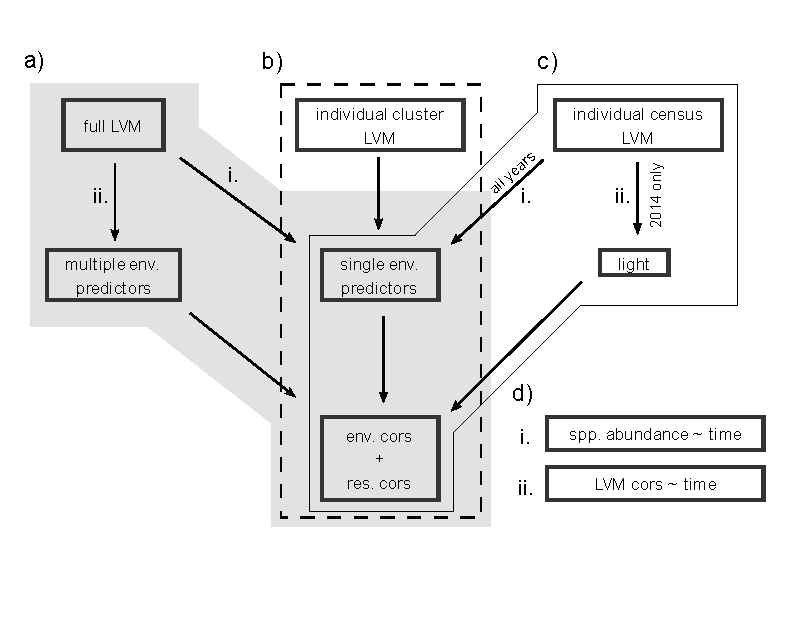
\includegraphics[width=1.0\linewidth]{Chapter5/Figures/schem2}
\caption{Schematic summary of core analysis. Environmental and residual correlations calculated  for: a) LVMs fitted to the full  dataset for i) each of the nine environmental predictors  independently, and ii) for multiple predictors in a single model; b) LVMs fitted to each individual cluster for each predictor independently; and c) i) LVMs fitted to each census for each predictor independently (all census years), and ii) additionally for light in 2014. Supplementary GAMMS were fitted for: d) i) species abundance as a function of time for comparison with the residual correlations from the multiple predictor model, and ii) for environmental and residual correlations from the individual census LVMs as a function of time.}
\label{fig:schem}
\end{figure}

Similar to other co-occurrence models such as JSDMs \citep[e.g.,][]{Ovaskainen2010, Clark2013, Pollock2014}, the extent to which species exhibit distinct environmental responses was inferred through a fitted regression model, specifically using the framework of generalized linear models. However, instead of employing an unstructured covariance matrix to account for the missing environmental covariates and/or biotic interactions \citep[as was done in][for instance]{Ovaskainen2010, Pollock2014}, LVMs utilize latent variables as a parsimonious means of modelling residual species correlation \citep[see also][]{Harris2015}. As such, we use the term `residual' in reference to remaining patterns in the data after accounting for one or more predictors, rather than in terms of its definition in the context of residual analysis. 

Our model can be regarded as an extension of the LVM proposed for model-based unconstrained ordination in \citet{Hui2014}, and can be written in the following hierarchical form:

\begin{align} \begin{aligned}[c] \label{eqn:basiclvm} 
\text{Responses:} &\quad [y_{ij} | \bm{u}_i, \bm{x}_i] \sim \text{Neg-Bin}(y_{ij}; \mu_{ij}, \phi_j) \\
&\quad \log(\mu_{ij}) = \eta_{ij} = \bm{x}'_i \bm{\beta}_j + \bm{u}'_i \bm{\lambda}_j \\
\text{Latent Variables:} &\quad [\bm{u}_{i}] \sim \mathcal{N}(\bm{0},\bm{I}) \\ 
\text{Priors:} &\quad [\bm{\beta}_j] \sim \mathcal{N}(\bm{0},c_0\bm{I}), \; [\bm{\lambda}_j] \sim \mathcal{N}(\bm{0},c_0\bm{I}), \; [\phi_j] \sim \text{Unif}(0,c_1), 
\end{aligned} \end{align}

where $`\sim'$ denotes ``is distributed as'', $\mathcal{N}(\cdot,\cdot)$ denotes a multivariate normal distribution with mean and covariance matrix given by the first and second arguments respectively, $\text{Unif}(0,c_1)$ denotes a uniform distribution with minimum zero and maximum $c_1$, and $\bm{I}$ denotes an identity matrix. To elaborate, $y_{ij}$ denotes the observed count for species $j$ at site $i$, and is assumed to come from a negative binomial (Neg-Bin) distribution with mean $\mu_{ij}$ and species-specific overdispersion parameter $\phi_j$. We used a negative binomial distribution as it exhibits a quadratic mean variance relationship, $\text{Var}(y_{ij}) = \mu_{ij} + \phi_j\mu^2_{ij}$, which allowed us to explicitly account for overdispersion present in the species counts.

Using a log-link function, the mean $\mu_{ij}$ was regressed against two sets of variables. Firstly, a vector of explanatory variables for each site, $\bm{x}_i$, which included an intercept term, environmental covariates (e.g. soil moisture), a fixed effect for the four clusters of plots to account for spatial non-independence within clusters (full and individual year models), and a random effect (intercept) for plot to account for temporal non-independence (full and individual cluster models). In order to account for unimodal species responses as predicted by niche theory \citep{Austin2002}, quadratic terms were included for the environmental covariates in each model. The second set of variables comprised a vector of two latent variables for each site, $\bm{u}_i = (u_{i1},u_{i2})$, which were assumed to be drawn from independent, standard normal distributions. The species-specific regression coefficients $\bm{\beta}_j$ and $\bm{\lambda}_j$ describe how the mean changes as a function of the explanatory and latent variables respectively.  

The key element in the LVM in equation (\ref{eqn:basiclvm}) are the latent variables $\bm{u}_i$, which can account for any residual correlation between species not attributable to spatial heterogeneity in the measured environmental covariates $\bm{x}_i$. This correlation may be driven by biotic interactions such as competition (negative) or facilitation (positive), or alternatively to missing predictors, where $\bm{\lambda}_j$ are the coefficients corresponding to these missing predictors. In addition, in our full model which combines multiple censuses, residual correlation may arise due to negatively or positively correlated fluctuations in species abundance through time. If unaccounted for, missing covariates, ecological interactions or temporal correlation will induce residual correlation between species which can potentially lead to erroneous inference. Latent variables offer an attractive approach to dealing with this issue. In particular, they require significantly fewer parameters to model species residual correlation compared to the unstructured (full rank) correlation matrices used by \citet{Ovaskainen2010} and \citet{Pollock2014}. Finally, note that more than two latent variables could have been used, although our preliminary testing with this dataset suggested that two was sufficient to characterize the main patterns of species residual correlations. 

We used Bayesian Markov Chain Monte Carlo (MCMC) methods to estimate the LVMs, with sampling performed through JAGS v3.4.0 \citep{plummer2003jags} using the package R2jags v0.03-08 \citep{su2012r2jags} in \texttt{R} v3.1.1. We assigned uninformative priors for all parameters, $\bm{\beta}_j, \bm{\lambda}_j$ and $\phi_j$, by setting $c_0 = c_1 = 100$ in equation (\ref{eqn:basiclvm}). For the full and individual cluster models, we also assigned an uninformative uniform prior for the variances of the random effect for plot. For each LVM fitted, we ran three chains with a burnin period of 10,000 iterations followed by 100,000 iterations with a thinning lag of 50 for each chain. This produced a final combined sample of 6000 MCMC samples for each LVM. We assessed parameters to have converged when traceplots were well mixed and the Gelman-Rubin statistic was below 1.1.

\texttt{R} code demonstrating the fitting and analysis of latent variable models of co-occurrence is provided in Appendix D.

\subsection*{Model inference and supplementary analysis}

After fitting the LVMs, in order to visualize patterns of co-occurrence arising from the different environmental factors, we calculated two types of correlation matrices. The first was constructed by calculating, for any two species, the correlation between their fitted values $\bm{x}'_i \bm{\beta}_j$ (across all plots). This is the same as equation (4) in \citet{Pollock2014}, with the resulting matrix representing the correlation between species that can be attributed to a shared/diverging environmental response. The second type of correlation matrix was calculated using the latent variable coefficients, $\bm{\lambda}_j$, also known as factor loadings. Specifically, if we let $\bm{\Lambda}$ be the two-column matrix formed by stacking the factor loadings on top of each other, then a covariance matrix is obtained as $\bm{\Lambda}\bm{\Lambda}'$ from which the residual correlation matrix can be calculated. This second residual correlation matrix represents the correlation between species that may be attributable to biotic interactions or missing environmental covariates. Since Bayesian MCMC estimation was used, the correlation between fitted responses was calculated for each MCMC sample, which made it possible to obtain a posterior distribution for each cell of the environmental and residual correlation matrix. As such, correlation `significance' was evaluated on the basis of the 95\% credible intervals for the posterior mean excluding zero. 


Having extracted environmental and residual correlation matrices for each environmental factor in each of the three model types (full, individual cluster, individual census point), we assessed the importance of each factor as a niche axis on the basis of two criteria: i) the number of significant negative pairwise environmental responses, where significance is defined as 95\% credible intervals that don't cross zero; and ii) the minimum number of species that need to be excluded to remove all negative pairwise responses, referred to in network theory as the minimum vertex cover. In this application, the minimum vertex cover quantifies the extent to which a given number \textit{n} of negative pairwise environmental responses is driven by one species exhibiting a different response to all other species, or at the other extreme consists of completely unique species pairs. In the former case, only one species need be excluded to remove all negative correlations whereas in the latter case $\textit{n}$ species must be removed. As such, with 12 species, if all 66 unique pairs exhibit significant negative correlations (an implausible scenario necessitating extremely narrow niche breadths), 11 would need to be excluded. In addition to quantifying negative pairwise environmental responses, we also counted the number of positive (shared) environmental responses to evaluate the extent to which a given environmental factor influences the fine-scale distribution of species even in the absence of any clear niche differentiation (e.g. if all species exhibit a similar response to the gradient). 

After considering species-specific environmental responses, we then examined the residual correlation matrix for each model, with particular emphasis on the full model including all of the environmental predictors, as this represents patterns of co-occurrence unexplained by all our measured predictors combined. To aid interpretation of the residual correlation matrix from the full multi-predictor model, we also fitted a generalized additive mixed model (GAMMs) for each species as a function of time, and compared the correlation in the fitted values from the GAMMs with the residual correlation matrix based on the full LVM model including multiple environmental predictors. The temporal GAMMs for each species were fitted using the MGCV package \citep{wood2012mgcv}, with a thin-plate spline smoother for time, a fixed effect for plot cluster, a random effect for plot, an AR(1) correlation structure nested within plot, and assuming a negative binomial error distribution with log link. If patterns in the residual correlation matrix of the full model are largely a product of temporal correlation (negative or positive) in species responses, we expected a strong correlation with the fitted value correlation matrix derived from the individual GAMMs. Correlation between the two matrices was assessed via a Mantel test. Note that the GAMM for one species, \textit{Empodisma minus}, failed to converge (most likely due to overdispersion), and as a result had to be excluded from the temporal analyses.

To investigate temporal trends in environmental and residual correlations, we also fitted GAMMs for mean pairwise environmental and residual correlation as a function of time for all variables combined. Each model included a thin-plate spline smoother for time, a random effect for environmental variable and an AR(1) correlation structure nested within environmental variable. Owing to the mean correlations values being consistently positive and right skewed, we used a gamma error distribution with a log link function. To correct over-smoothing observed in the residual correlation trends model, the maximum number of degrees of freedom was reduced from 9 (package default) to 4.

Finally, we performed \textit{post-hoc} exploratory analysis of the differences in species response to soil moisture with their pairwise differences in two readily available aboveground traits, plant height and seed mass. In each case, we used a Mantel test to compare pairwise difference in soil moisture (-1 x environmental correlation) with pairwise trait differences, and visualised the relationship with scatterplots.    

\section{Results}

Of the nine environmental variables considered independently in each of the single-predictor models for the full dataset, all but pH produced significant negative correlations due to diverging species-specific responses (Fig. \ref{fig:networkplots-negfull}). Deep soil-moisture was associated with both the largest number of negative correlations (18) and the largest number of node removals required to eliminate all negative correlations (4). As is to be expected given such strong correlations, the 12 species displayed a range of differentiated responses to the deep soil-moisture gradient, with some increasing monotonically (or near monotonically) towards the extremes of the gradient (e.g. \textit{Xanthorrhoea resinosa}, \textit{Haemodorum corymbosum} and \textit{Entolasia stricta}), whilst others exhibited unimodal peaks closer to the middle of the gradient (e.g. \textit{Ptilothrix deusta}, \textit{Empodisma minus} and \textit{Xyris gracilis}) (Fig. \ref{fig:responsefig_cred}). Exchangeable aluminium was associated with the second largest number of negative correlations (17), followed by organic carbon (11), shallow soil-moisture and total iron (10), exchangeable magnesium (6), cation exchange capacity (3), and phosphorous (1) (Fig. \ref{fig:networkplots-negfull}). Whilst pH was not associated with any negative pairwise correlations, 27 species pairs exhibited significant positive correlations to pH. Deep soil-moisture was associated with the second highest number of significant positive correlations, followed by exchangeable aluminum and exchangeable magnesium (21), organic carbon (18), shallow soil-moisture (17), total iron (16), cation exchange capacity (12), and phosphorous (8) (see Fig. S5.1 in Appendix D).
 
 \begin{figure}[H]
 \centering
 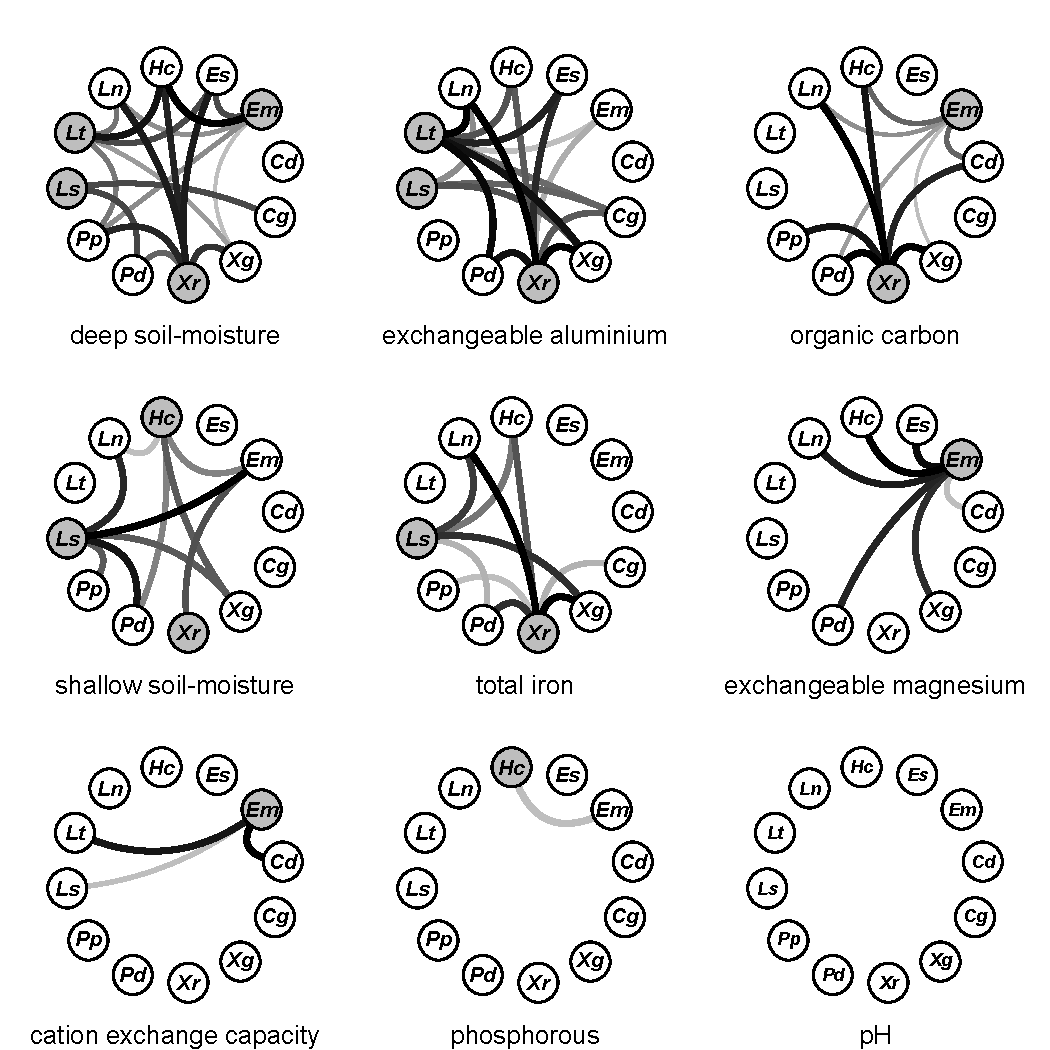
\includegraphics[width=1.0\linewidth]{Chapter5/Figures/networkplots-negfull}
 \caption{Negative pairwise species correlations to the environment derived from single-predictor LVMs for the full dataset. Connecting lines between species nodes denote negative mean posterior correlations with credible intervals excluding zero. Line colour and thickness indicates the strength of the negative correlation where darker and thicker lines are closer to -1. Nodes shaded grey indicate the minimum vertex cover, i.e. the smallest combination of species that need to be removed to break all negative associations (note that while the minimum number has a single solution, the species composition making up the minimum vertex cover set can vary). Species node labels combine the first letters of the genus and specific epithet given in full in Fig. \ref{fig:responsefig_cred}.}
 \label{fig:networkplots-negfull}
 \end{figure}
 
 \begin{figure}[H]
 \centering
 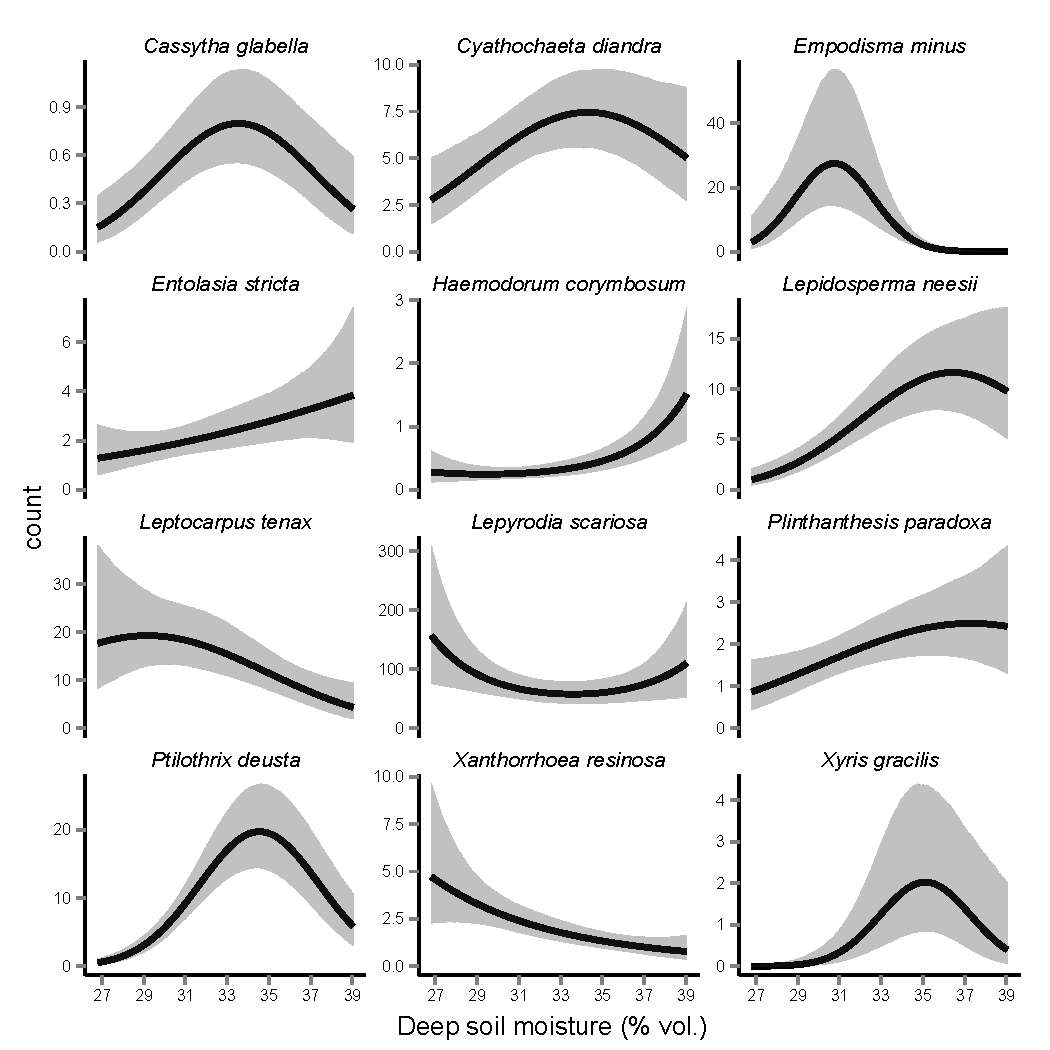
\includegraphics[width=1.0\linewidth]{Chapter5/Figures/responsefig_cred_mcmc}
 \caption{Species specific responses to the deep soil-moisture gradient. Fitted values derived from regression parameter estimates from the deep soil-moisture LVM (full dataset). Shaded region denotes 95\% credible intervals.}
 \label{fig:responsefig_cred}
 \end{figure}



Residual correlations based on single-predictor LVMs fitted to the full dataset were strongly associated with each other, and with residual correlations from the multi-predictor model (\textit{r} = 0.68-0.97). As such, the consistency of the observed residual correlations suggests a potentially important variable was not accounted for in any of the LVMs. Nevertheless, most of the significant correlations in the residual correlation matrix  of the multi-predictor model were positive (23) rather than negative (2), thus negating the probability that an important fine-scale niche axis was omitted from our analysis (Fig. \ref{fig:multiresid}). Furthermore, a substantial portion of the residual correlation appears to be attributable to shared and differentiated temporal responses between species, with the residual correlation matrix from the multi-predictor model being moderately associated with the temporal response correlation matrix derived from the temporal models (Mantel test \textit{r} = 0.43) (see Fig. S5.2 for smoothed species responses through time).



\begin{figure}[H]
\centering
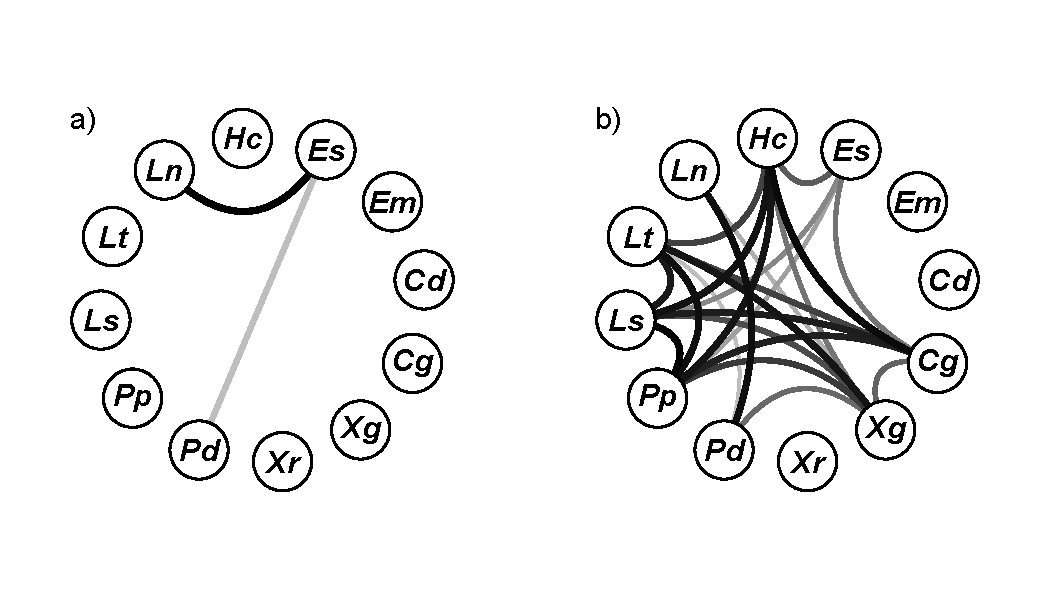
\includegraphics[width=0.7\linewidth]{Chapter5/Figures/multiresid}
\caption{Negative (a) and positive (b) pairwise residual correlations derived from the multi-predictor LVM for the full dataset. Connecting lines between species nodes denote posterior correlations with credible intervals excluding zero. Line colour and thickness indicates the strength of the correlation where darker and thicker lines are closer to $|1|$. Species node labels combine the first letters of the genus and specific epiphet.}
\label{fig:multiresid}
\end{figure}



Relative to the models run on the full dataset, the number of significant negative correlations due to diverging environmental responses between species was considerably smaller for models run on each individual cluster (plots separated by 5-45 metres). As such, most of the observed patterns of co-occurrence in the full models appears to be driven by environmental variation over spatial scales of 10s of metres, rather than metres (i.e. between clusters rather than within clusters). The one exception to this pattern was for phosphorous, which exhibited a relatively high number of significant negative co-occurrence associations in three of the four clusters. Notably, a substantial number of species did exhibit negative pairwise associations in the residual correlation matrices for at least two of the clusters, suggesting that biotic interactions may still influence co-occurrence at within-cluster scales (see Table S1).

The number of significant negative pairwise associations in species environmental response was also comparatively small for the individual census models. It is notable however that even if we ignore `significance' criteria, the sign of each pairwise species association is largely consistent with those observed for the single predictor models for the full dataset. In addition, the models for each individual census provide insight into the relative dominance of positive and negative interactions through time. Whilst there were no obvious trends in mean environmental correlation through time, residual correlations underwent a conspicuous upwards positive trend in the second half of the sampling period (Fig. \ref{fig:temptrends}). Pairwise species associations derived from the single LVM fitted for light availability in 2014 were almost universally positive, with all but one species (\textit{Xanthorrhoea resinosa}) being more abundant in less shaded locations. 

\begin{figure}[H]
\centering
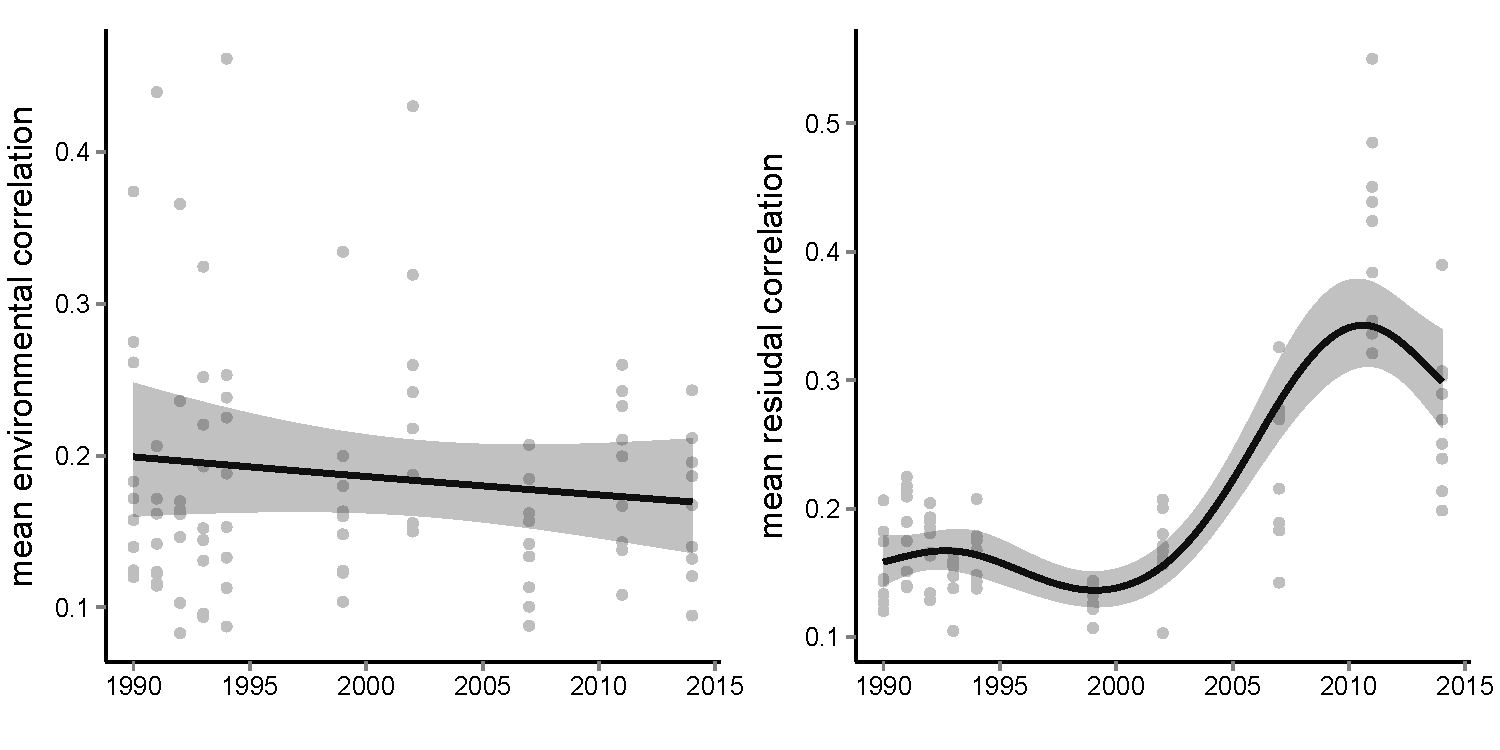
\includegraphics[width=1.0\linewidth]{Chapter5/Figures/temptrends}
\caption{Trends in mean environmental (left) and residual (right) correlation through time. Trend lines obtained with thin-plate splines in a GAMM framework (see main text for model fitting). Shaded region represents 95\% confidence intervals.}
\label{fig:temptrends}
\end{figure}



Differences in species pairwise responses to deep soil moisture were moderately positively related to pairwise difference in plant height (\textit{r} = 0.6259, \textit{P} = 0.002) but unrelated to differences in seed mass (\textit{r} = -0.1176, \textit{P} = 0.809) (Fig. \ref{fig:traits_diffs}). 

\begin{figure}[H]
\centering
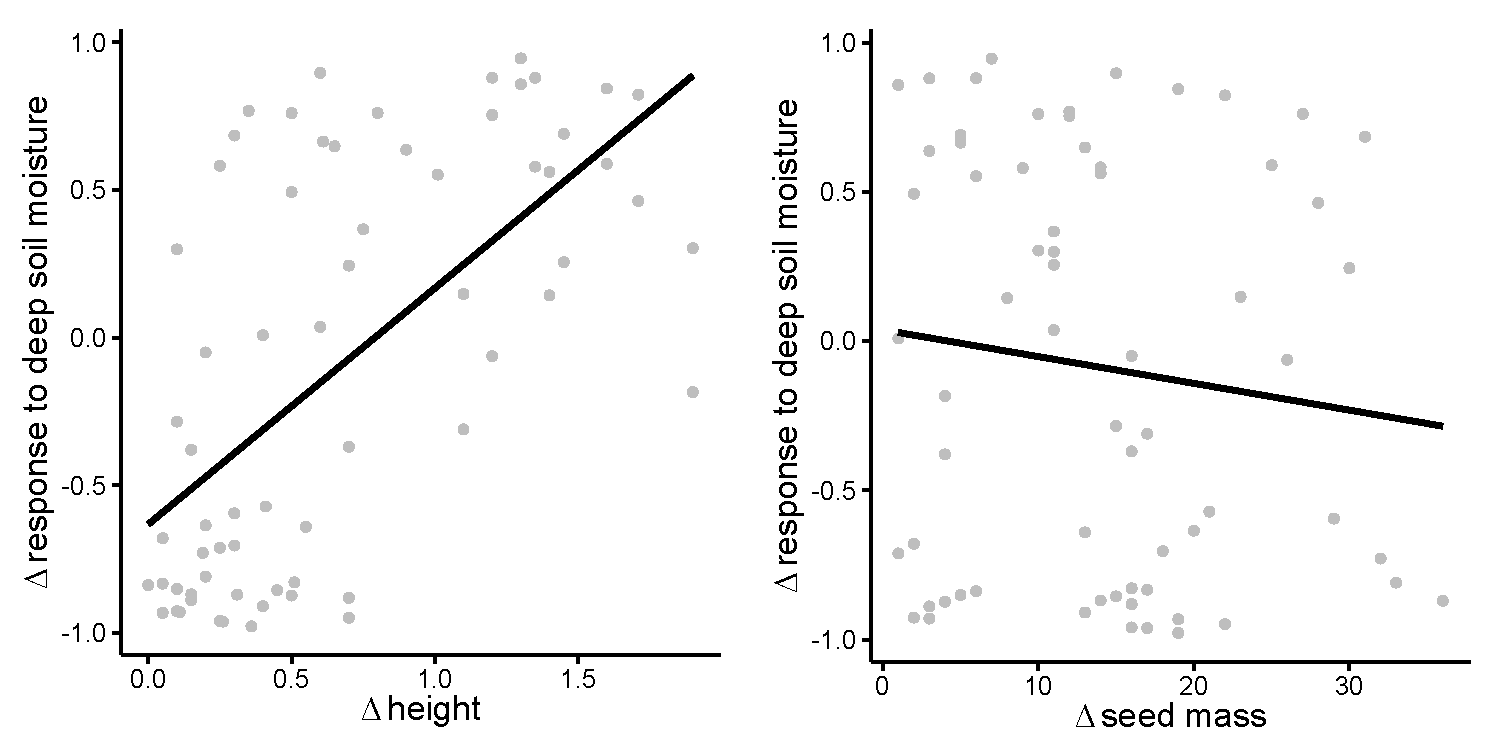
\includegraphics[width=1.0\linewidth]{Chapter5/Figures/traits_diffs}
\caption{Scatterplots of pairwise differences in species responses to deep soil moisture (-1 x environmental correlation) in relation to pairwise difference in plant height (left) and seed mass (right). Lines of best fit obtained from linear models.}
\label{fig:traits_diffs}
\end{figure}

\section{Discussion}

The notion that fine-scale spatial environmental variability may foster plant species coexistence is founded upon a rich body of theory \citep{Chesson2000, Amarasekare2003, Adler2013}, and yet empirical efforts to establish which, if any, environmental factors are associated with strong patterns of fine-scale niche differentiation are surprisingly sparse. We found strong empirical support for the hypothesis that differentiation along hydrological gradients represents one of the most important fine-scale plant niche axes at within-community scales \citep[\textit{sensu}][]{Silvertown2015}. On the basis of multiple criteria, deep soil moisture emerged as the single best predictor of negative co-occurrence patterns (Fig. \ref{fig:networkplots-negfull}), with the dominant community members exhibiting strongly differentiated responses across a comparatively narrow moisture gradient (Fig. \ref{fig:responsefig_cred}). Together with several earlier studies \citep[e.g.][]{Silvertown1999, Araya2011}, these results are amongst the first to demonstrate hydrological niche differentiation in the absence of significant topographical complexity. Furthermore, they highlight the robustness of the hypothesis when confronted with a comprehensive set of alternative prospective niche axes.

The adoption of a latent variable modelling framework enabled us to not only evaluate the comparative importance of each environmental factor, but also to determine the likelihood that an important factor was unaccounted for. Given that the residual correlation matrix from the multi-predictor model was dominated by positive pairwise associations, we can be confident that we accounted for the most important factors driving niche segregation amongst the dominant community members (Fig. \ref{fig:multiresid}). As such, our approach allows robust conclusions about the relative importance of soil hydrology not only with respect to measured variables but also unmeasured variables. Notably, a considerable portion of the residual correlation from the multi-predictor model appeared to be attributable to both positive, and to a lesser extent negative, temporal correlations in species peak abundance. These in turn appear to largely reflect differential interspecific temporal responses to fire events in 1988, 1994 and 2001 (Fig. S5.2). As such, with time-series data, co-occurrence models may also be used to draw inferences on successional processes and temporal niche partitioning. 

While the results provide strong evidence for fine-scale hydrological niche differentiation, the extent to which hydrological niches provide opportunities for local-scale species coexistence is to a large extent contingent on the scale at which the community is defined \citep{Amarasekare2003, Adler2013}. For instance, in the current study, negative co-occurrence patterns associated with the deep soil moisture gradient were only detectable when comparing plots across clusters separated by 100-320 metres. Similarly, \citet{Silvertown1999} made what is probably the strongest case for hydrological niches to date on the basis of plots dispersed across 10's of hectares, whilst even the ca. 50 x 50 metre plots of \cite{Araya2011} presumably allowed for individuals to be spaced as much as 70 metres apart. In contrast, \citet{Fridley2011} reported species-specific responses to microsite variation in soil depth in 3 x 3 metre plots in a limestone grassland, but this appeared to be unrelated to soil water potential. As such, the evidence for hydrological niches at the local scale within which neighbouring plants directly compete for resources arguably remains relatively weak. This conclusion would be in line with the dominant paradigm in community ecology that negative patterns of co-occurrence at the local scale are predominately indicative of competitive exclusion \citep[][but see Fridley \textit{et al.} 2011]{Gotelli2002}. Indeed, only phosphorous exhibited more than six negative pairwise associations (compared with just one for the full dataset) in any one plot cluster (Table S5.1). In contrast, the residual correlation matrices for two plot clusters exhibited a relatively large number of negative associations, which do not appear to be driven by any of the measured environmental factors. Nevertheless, even in the absence of localised spatial partitioning of resources, hydrological niches may still promote local coexistence via source-sink dynamics and spatial storage effects \citep{Shmida1984, Amarasekare2003, Snyder2004}. This will arise when species are able to disperse from favourable to less favourable locations at a sufficiently high rate to offset locally negative population growth rates and thus prevent local extinction \citep{Snyder2004}. Since monitoring began in the current study, all but one species has been recorded at all four clusters, suggesting that most of the dominant community members do indeed regularly disperse to and establish in locations where they are less competitive. It is also notable, that within short distances ($<$100 m) of our study plots, the topography is more varied, and as such may provide nearby opportunities for even finer scale hydrological niche differentiation. 

In contrast to the individual plot cluster models, the lack of strong negative environmental correlations in the individual census models appears to be an artefact of low power, particularly given that the raw correlation values corresponded closely with those from the full model. Nevertheless, it is interesting to note that whereas mean environmental correlations were relatively static through time, residuals correlations exhibited a strong upwards trend towards more positive values (Fig. \ref{fig:temptrends}). This trend most likely reflects a shared environmental response to increased overstorey shading, as indicated by the observed positive response of the majority of species to light availability in the most recent 2014 census. In a previous study from the same site, \citet{Letten2014a} described an increase in functional and phylogenetic similarity of community members through temporal succession consistent with this observation.

Our focus was on negative environmental correlations, but positive correlations also provide insight into other aspects of community assembly. For instance, positive correlations in species responses were highest for soil pH, suggesting pH may be a useful predictor of local richness patterns, whilst also acting as niche axis over larger spatial scales. It is also notable that although this system is typically associated with low-pH adapted species, many of the dominant herbaceous community members exhibited a positive response to the pH gradient (data not shown). As such, it would be interesting to explore the extent to which rarer species exploit this apparently `unoccupied' niche space within the landscape, particularly given the known importance of soil pH for plant community structure in other systems \citep{Laliberte2014}.

Although a comprehensive examination of trait-environment relationships was beyond the scope of this study, comparisons of species pairwise differences in seed mass and plant height relative to hydrological niches differences still proved informative. Whereas differences in seed mass, which may be associated with survival from drought stress \citep{Perez-Harguindeguy2013}, were unrelated to hydrological niches, differences in plant height were strongly positively related with differences in species response to soil moisture (Fig. \ref{fig:traits_diffs}; cf. Fig 2c in Adler \textit{et al.} 2013). This appeared to be driven predominately by taller species (e.g \textit{Leptocarpus tenax} and \textit{Xanthorrhoeaa resinosa}) favouring drier areas of the deep soil moisture gradient, while shorter species (e.g \textit{Plinthanthesis paradoxa} and \textit{Xyris gracilis}) were more abundant in wetter areas. This we expect reflects the greater tolerance of shorter species to anaerobic conditions in periodically saturated sites. Given that soil moisture measurements at all depths were typically around, or above, the field capacity of sandy-loam soil ($\sim$23\% vol., \citealp{atwell1999plants}), this possibly reflects the greater tolerance of shorter species to low oxygen in periodically saturated sites. In addition it suggests fine scale variability in soil moisture may have important implications for the structural complexity of standing vegetation.

Beyond differences in plant height and seed mass, it is notable that the dominant herbaceous members of the community actually exhibit remarkably similar phenotypes, with all but one of the twelve study species being a geophytic or hemicryptophytic monocot, and nine of the twelve belonging to just three families within the poales (\textit{Restionaceae}, \textit{Poaceae} and \textit{Cyperaceae}). This apparent constraint on functional strategies is likely attributable to the fire-prone and nutrient poor nature of the system, which makes it all the more remarkable that these same species exhibit such differentiated responses to the soil moisture gradient. One likely explanation is that these species exhibit a range of different below-ground adaptations to water acquisition and flooding/drought tolerance \citep{Silvertown2015}. 

An open question arising from our results is why species co-occurrence patterns should exhibit a stronger relationship with deep, rather than shallow, soil moisture. This is particularly true given that most of the study species are likely to have the bulk of their rooting volume above 1,000 mm where the deep soil moisture measurements were made. The most parsimonious explanation is that shallow soil moisture is unevenly modified by plant water usage and episodic rainfall recharge, and thus provides a poorer approximation of baseline soil moisture across the study area. More specifically, shallow soil moisture is likely to experience greater seasonal and interannual variability contingent on the density of standing vegetation. Observed trends in monthly soil moisture support this notion, with shallow soil moisture exhibiting a relatively strong seasonal trend over the 12 months of sampling, which appeared to be mostly attributable to increased plant water usage over spring/summer rather than decreased rainfall. In contrast, deep soil moisture was comparatively stable. This may explain the apparent lack of a strong relationship between species specific responses and near surface soil moisture observed by \citep{Fridley2012}. Ultimately, the depth of soil moisture that best predicts hydrological niches is likely to depend on numerous system-specific factors, but our findings highlight the potentially confounding role of plant water usage on inferences drawn from near surface measurements. Furthermore, it is notable that elevation was a poor predictor of soil moisture at any depth, confirming that the use of terrain-based hydrological models in plant niche studies may lead to misleading conclusions.

One challenge to interpreting plant compositional responses to spatial variability in soil moisture is the dual role of water as both a depletable resource factor (cf. nutrients or light) subject to density-dependent feedbacks and as a non-resource factor (cf. temperature or soil type) that mediates density-independent responses (e.g. via reduced oxygen diffusion). It follows that depending on supply rates, spatial heterogeneity in soil moisture may produce complex interactions between niche and fitness differences amongst interacting species \citep[\textit{sensu}][]{Chesson2000}. It might therefore be expected that the breadth of plant responses to soil moisture will allow for higher-dimensional trade-offs relative to more narrowly defined environmental factors \citep{tilman1982, Chase2003}. In the current study, soil moisture appeared to be consistently around or above the likely field capacity of the soil. This suggests that in this system soil moisture may exert a stronger influence on compositional patterns by acting as a stressor rather than a spatially heterogenous limiting resource. In the absence of data on spatial variation in air-filled porosity such inferences are unfortunately somewhat speculative, but this represents an important consideration for future studies.

It is important to recognise that demonstrating species-specific environmental responses along a given gradient, is not on its own sufficient evidence that it facilitates species coexistence. To this end, rigorous tests of species coexistence necessitate experimental manipulations of intra- and inter-specific competition \citep[e.g.][]{Levine2002, Sears2007a, Godoy2014}, or alternatively the mathematical parametrization of models from long-term demographic studies \citep[e.g.][]{Adler2006, Angert2009}. Unfortunately these approaches are not always practical, particularly in perennial systems such as heathlands where individuals can take several years to reach reproductive maturity. Nevertheless, as advocated by \citep{Silvertown2015}, providing evidence of fine-scale hydrological niche differentiation is an important first step, that will hopefully provide stimulus for further research.

Here we have provided robust evidence for species-specific responses to fine-scale variation in soil hydrology, whilst also illustrating the valuable inferential gains made possible with model-based approaches to co-occurrence analysis. Our results are consistent with emerging empirical evidence, but go a step further than previous studies by demonstrating the apparent strength of hydrological niche differentiation when compared to a range of other potential niche axes. Future research efforts should focus on identifying the different physiological processes and traits associated with hydrological niches \citep{Silvertown2015}, and on exploring scale dependencies to better understand the underlying coexistence mechanisms at play \cite{Adler2013}. In light of perturbations to hydrological regimes under climate change, a better understanding of hydrological niches could prove critical to conservation efforts.


\section*{Acknowledgements}

For their assistance with fieldwork we are grateful to Chantel Benbow, Sam Dawson, Chris Gordon, Anna Feit, Ben Feit, Sylvia Hay, Mitch Lyons and Max Mallen-Cooper. Thanks also to Martin Westgate whose `circleplot' package was used to produce the network plots in Fig. 1.

\newpage



%\section{水方halfhda速度6未来发展}
\subsection{已知问题}
本模板未采用2013版规范的页边距设置,因为实在是办不到2.5CM顶部页边距加上2.6CM的页眉设置啊。
\subsection{未来发展}
武汉理工大学本科生论文的未来发展还是需\cite{MartinDSP00}要各位用户的参与,如果每一个用户都能贡献出一点关于\LaTeX 模板的想法和意见,我相信几年之后武汉理工大学本科生论文模板会成为其他高校学习和借鉴的例子。同学当自强,让我们一起来丰富完善这个模板,如果你有很好的建议或者意见请发送到 thesis@tsaoyu.com
\subsection{官方认证}
到目前为止(\today )没有武汉理工大学任何官方组织\cite{吴昉张页-222}对于本模板的格式或者内容进行认证,这代表采用本模板进行的论文写作可能不被官方的论文系统接受。如在进行原创性(防抄袭)检测的时候,可能需要提供提供doc版本的论文。希望用户了解到这个潜在的风险,做好文件转换和备份的准备。本人不对任何由于使用本模板而导致的毕业论文纠纷承担任何责任!
\subsection{测试代码}
%%   插入表格
%%   \hline                            表示横线
%%   \\                                表示换行
%%   \begin{center}   \end{center}     表示表格居中
%%   \centering                        表示表格居中
%%    [!h]    [H]                         固定表格位置
%% 	  \caption{}                       表格自动标号
%%选中若干表格
\begin{table}[H]
\begin{center}
\begin{tabu}{|c|c|c|c|c|}
\hline
foo & foo & foo & foo & foo \\
\hline
foo & foo & foo & foo & foo \\
\hline
foo & foo & foo & foo & foo \\
\hline
\tikzbox{foo} & {foo} &{foo} & {foo} & \tikzbox{foo} \\
\hline
foo & foo & foo & foo & foo \\
\hline
foo & foo & foo & foo & foo \\
\hline
foo & foo & foo & foo & foo \\
\hline
\tikzbox{foo} & \tikzbox{foo} & \tikzbox{foo} & \tikzbox{foo} & \tikzbox{foo} \\
\hline
\end{tabu}
\end{center}
\end{table}

%%两个并列的表格,连在一起写即可(比较窄的表格)
\begin{table}[H]
\begin{center}
\noindent\begin{tabular}{*{3}{c}}
\hline
Header1 & Header 2 & Header3 \\
\hline
Column1a & Column2a & Column3a \\
Column1b & Column2b & Column3b \\
Column1c & Column2c & Column3c \\
Column1d & Column2d & Column3d \\
\hline
\end{tabular}\quad           %% 两个表格的分界线
\begin{tabular}{*{3}{c}}
\toprule
Header1 & Header 2 & Header3 \\
\midrule[2pt]
Column1a & Column2a & Column3a \\
Column1b & Column2b & Column3b \\
Column1c & Column2c & Column3c \\
Column1d & Column2d & Column3d \\
\bottomrule
\end{tabular}
\end{center}
\end{table}

%%一般意义的正常表,表格自动标号\caption{}
\begin{table}[H]       %%表格插入到当前位置【h】,【!】表示不考虑美学
\caption{kdjakjdfkajd}  %%caption内部是表格的题注
\centering
\begin{tabular}{cc}
\toprule
Header1 & Header 2 \\
\midrule[2pt]
Column1a & Column2a  \\
Column1b & Column2b  \\
Column1c & Column2c \\
Column1d & Column2d \\
\bottomrule
\end{tabular}
\end{table}

%%具有行列合并的表格
%%建议先复制这段代码跑出表格,然后分析代码
\begin{table}[H]   %%【htb】,表格插入到here,top或者bottom
\caption{kdjakjdfkajd}
\centering
\begin{tabular}{c|cc}
\toprule
Header1 & Header2 & Header3 \\
\midrule[2pt]
\multicolumn{3}{c}{\textbf{Column1a} } \\             %行合并(合并第一行)
Column1b & Column2b & \multirow{3}{*}{\tabincell{c}{the first line \\ the next}} \\     %%列合并
Column1c & Column2c \\
Column1d & Column2d &  \\
\bottomrule
\end{tabular}
\end{table}

%% 美赛表格汇总
%%变量表
\begin{table}[H]
\caption{Symbol Table-Variables1}
\centering
\begin{tabular}{lll}
\toprule
Symbol & Definition  & Units\\
\midrule[2pt]
\multicolumn{3}{c}{\textbf{Variables} }\\
\multirow{3}{*}{\tabincell{l}{  $N$  } }& \multirow{3}{*}{\tabincell{l}{the first lineThe number of vehicles\\ passing a certain point on the highway } } & \multirow{3}{*}{\tabincell{l}{ unitless} }  \\
\\
\\
$L$ & Lenth of cell & cell   \\
${c_i}$ & The serial number of cell (Number i)   & unitless\\
$({r_i},{c_i})$ & the position of cell(Number i) & unitless\\
${r_{i}}$ & The serial number of Lane(Number i) & unitless\\
${r_{ti}}$ & The serial number of Target Lane(Number i) & unitless\\
$Head({r_i},{c_i})$ &Front gap  & cell\\
${Head_{side}}({r_i},{c_i})$ & Side front gap & cell\\
$Back({r_i},{c_i})$ & Back gap  & cell\\
${Back_{side}}({r_i},{c_i})$ &Side back gap  & cell\\
${v_i}$ &  The current speed of car(Number i)& cell/time-step\\
${v_{ti}}$ &The target speed of car(Number i)  & cell/time-step\\


\bottomrule
\end{tabular}
\end{table}
%%----------------------------------------------
\begin{table}[H]
\caption{Symbol Table-Variables2}
\centering
\begin{tabular}{lll}
\toprule
Symbol & Definition  & Units\\
\midrule[2pt]
${v_{limit}}$ &Maximum speed limit  & cell/time-step\\
$ v_{mean}$ &Average speed&  cell/time-step \\
${{\bar v_i}}$ &  Average speed(Number i)& cell/time-step\\
${p_{brake}}$ &  Probability of Accidental braking & unitless\\
${p_{Lc}}$ & Probability of Lane-Changing & unitless\\
${\theta }$ &The percentage of self-driving car  & unitless\\
${\tau }$ & Friendliness coefficient & unitless\\
${ \delta}$ & The extent of the back car affected & unitless\\
$\lambda$  & Expectancy of poisson-distribution & unitless  \\
${l_{a,safe}}$ &Safe distance of self-driving-car& cell\\
${l_{n,safe}}$ &Safe distance of None-self-driving car& cell\\
\multirow{2}{*}{\tabincell{l}{  $NL$  } }& \multirow{2}{*}{\tabincell{l}{the number of lanes } } & \multirow{2}{*}{\tabincell{l}{ unitless} }  \\
\\
$\Omega  $ & Lane changing algorithm & unitless\\
$\xi$  &Traffic flow over a period of time &  cell \\
${\xi _d}$&Average daily traffic volume& cell \\
${\xi _p}$&Traffic flow during peak hours& cell \\
$T$ &Iteration time& time-step\\
$t$&Iterative time slot & time-step\\
$DL$ & the number of dedicated lane&  unitless \\
$ L_{safe}$  & Average safe distance &  cell \\
$ L_{average}$  &Average vehicle length &  cell \\
$\eta$ &Average vehicle flow efficiency& unitless \\ 
\bottomrule
\end{tabular}
\end{table}
%%----------------------------------------------
\begin{table}[!h]
\caption{ Detailed configuration}
\centering
\begin{tabular}{ll|ll}
\toprule
Index &  value  & Index & value\\
\midrule[2pt]
$NL$ & 1/2/3   &$\theta $     & [0,1]\\
$L$ & 1000cell    &$\lambda  $    &\{0.1,0.25,0.5,10\} \\
$\tau$ &[0,1]   &${v_{limit}}$  &  10cell/time-step\\
 \multirow{2}{*}{\tabincell{c}{$\Omega  $}}  &  \multirow{2}{*}{\tabincell{c}{CCL/NCL/ACL/\\FCL}}&  $DL$  &  0/1/2/3  \\
 \\
\bottomrule
\end{tabular}
\end{table}
%%----------------------------------------------
\begin{table}[H]
\caption{ 中文表}
\centering
\begin{tabular}{ll|ll}
\toprule
项目 &  取值  &项目 & 取值\\
\midrule[2pt]
$NL$ & 1/2/3   &$\theta $     & [0,1]\\
$L$ & 1000cell    &$\lambda  $    &\{0.1,0.25,0.5,10\} \\
$\tau$ &[0,1]   &${v_{limit}}$  &  10cell/time-step\\
 \multirow{2}{*}{\tabincell{c}{$\Omega  $}}  &  \multirow{2}{*}{\tabincell{c}{CCL/NCL/ACL/\\FCL}}&  $DL$  &  0/1/2/3  \\
 \\
\bottomrule
\end{tabular}
\end{table}

%%单独一个图片
\begin{figure}[H]
\small
\centering
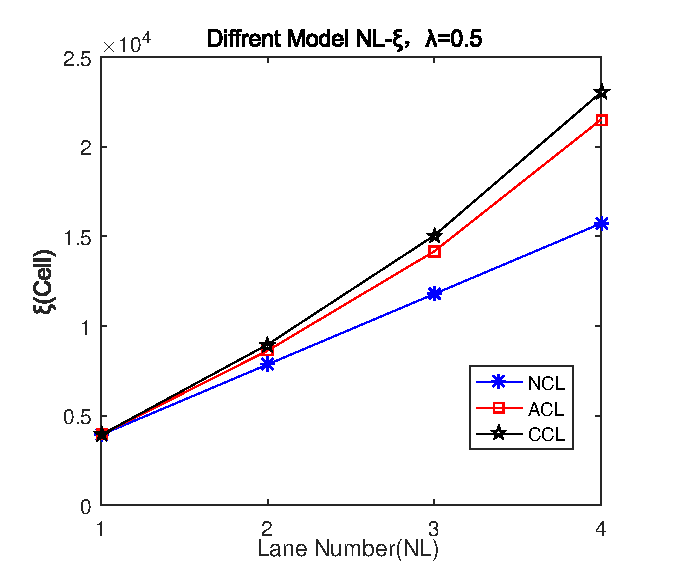
\includegraphics[width=8cm]{figure/421.eps}
\caption{a picture} \label{fig:a picture}
\end{figure}

%%插入两个并列图片4221和4222
\begin{figure}[H]
\centering
\subfigure[None dedicated lane]{
\label{figa} %% label for first subfigure
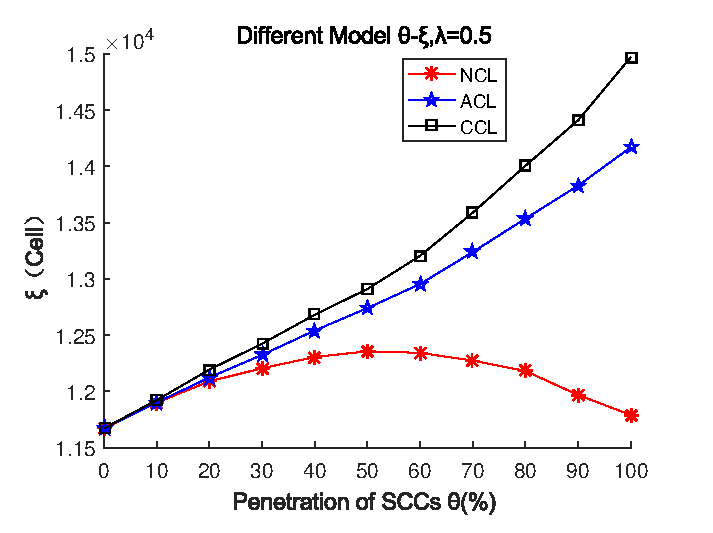
\includegraphics[width=5.3cm]{figure/4221.eps}}
\hspace{0cm}
\subfigure[Dedicated lane]{
\label{fig:subfig:b} %% label for second subfigure
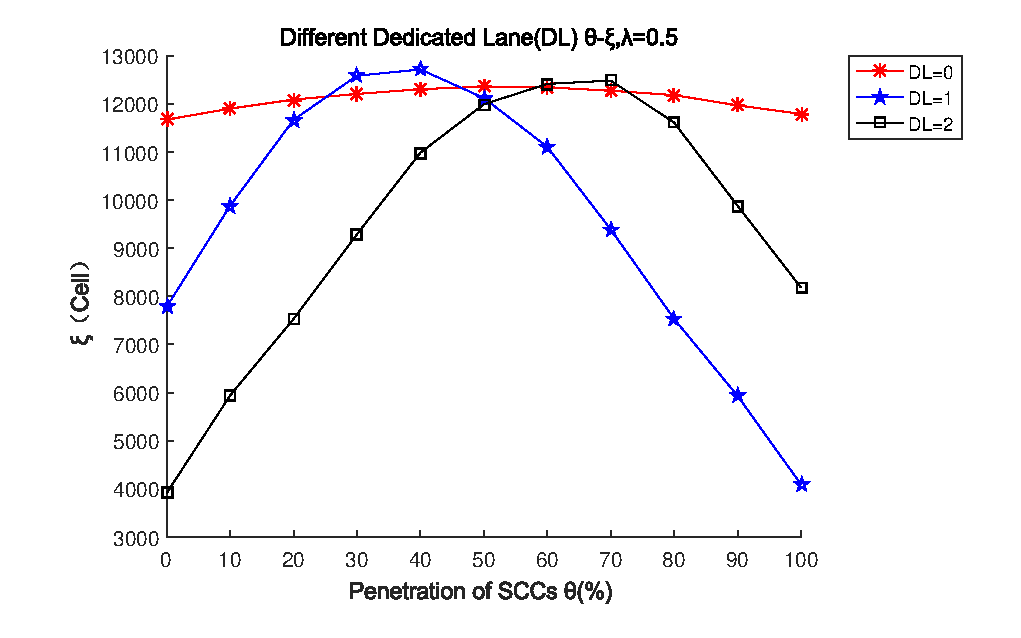
\includegraphics[width=6.6cm]{figure/4222.eps}}
\caption{Simulation Results for NCL,ACL,and CCL}
\label{figb} %% label for entire figure
\end{figure}


%%以下为定理代码
\begin{Theorem} 
for i>0, i++.
\end{Theorem}

%%以下为引理代码
\begin{Lemma} 
\TeX .
\end{Lemma}

\begin{Lemma} 
\TeX .
\end{Lemma}

\begin{Lemma} 
\TeX .
\end{Lemma}

\begin{Theorem} 
for i>0, i++.
\end{Theorem}

%%以下为证明
\begin{proof}
The proof of theorem.
\end{proof}

%%不一定要会,因为可以用mathtype写出公式之后导出latex代码
%%但是有时mathtype的公式导出时会出bug
%%所以建议还是看一看


%%公式输入,熟悉角标即可(常用)
%%    \]   和  $$  都是无编号的公式输入
%%      \begin{equation}  是有编号的输入
\begin{equation}
\sum\limits_{i = 1}^n {X_i^2} \sum\limits_{i = 1}^n {{X_i}{Y_i}} \frac{1}{n}\sum\limits_{i = 1}^n {{{({X_i} - \bar X)}^2}}       
\end{equation}

%%左对齐连续等号
\begin{equation}
\begin{array}{lllll}
 & \frac{{\delta y}}{{\delta x}}\\
{\rm{ = }} & \mathop {\lim }\limits_{\delta x \to 0} \\
{\rm{ = }} & \sum\limits_{i = 1}^n {{X_i}{Y_i}} \oint_S x dx\\
{\rm{ = }} & \sum\limits_{i = 1}^n {{{({X_i} - \bar X)}^2}} 
\end{array}
\end{equation}           %% 带上标号

%%矩阵
\[\left( {\begin{array}{*{20}{c}}
{{a_1}}&{}&0\\
{}& \ddots &{}\\
0&{}&{{a_n}}
\end{array}} \right)\left( {\begin{array}{*{20}{c}}
1&0\\
0&1
\end{array}} \right)\left( {\begin{array}{*{20}{c}}
{{a_{11}}}& \ldots &{{a_{1n}}}\\
 \vdots & \ddots & \vdots \\
{{a_{m1}}}& \cdots &{{a_{mn}}}
\end{array}} \right)\]


%%大括号分类
\[\left\{ \begin{array}{l}
ad\\
adf\\
adfa
\end{array} \right.\]

\begin{equation}
{p_{Lc,i}} = f({\delta _j},\tau ) = \left\{ \begin{array}{l}
1    ,{\delta _j} = 0\\
0   , {\delta _j} = 1\\
\max ( - \frac{\tau }{{1 - \tau }} \cdot {\delta _j} + 1,0){\rm{     }},otherwise{\rm{ }}
\end{array} \right.
\end{equation} 


\begin{equation}
{P_t}(n) = \frac{{{\lambda ^n}}}{{n!}}{e^{ - \lambda }}(n > 0)
\end{equation}
The $\lambda$ indicates the number of vehicles per unit time t. Let $ \lambda = \alpha t $, and $\alpha$ represents the average arrival rate of the vehicle. The Poisson distribution formula $(4.1)$ can be transformed into:
 \begin{equation}
{p_n}(t) = \frac{{{{(\alpha t)}^n}}}{{n!}}{e^{ - \alpha t}}(t > 0)
\end{equation}

%%无序列举
\begin{itemize}
\item  我的号哈佛的
\item  马上量很大
\item  撒考核法开始的恢复
\end{itemize}


%%加粗列举(看起来会很赞)
\begin{itemize}
\item \textbf{好的卡焦点科技几点开始}
\item \textbf{阿发达}
\item \textbf{看了就烦对哦}
\end{itemize}
%% this file is called up by thesis.tex
% content in this file will be fed into the main document

%: ----------------------- introduction file header -----------------------

\graphicspath{{7/figures/}} % specifies where the figures are stored

% ----------------------------------------------------------------------
%: ----------------------- content ----------------------- 
% ----------------------------------------------------------------------

\chapter{\label{ch7}Name of chapter 7} % top level followed by section, subsection

\section{\label{7:1}Name of section}

\subsection{\label{7:1:1}Name of subsection}



% ---------------------------------------------------------------------------
%: ----------------------- end of thesis sub-document ------------------------
% ---------------------------------------------------------------------------


%% this file is called up by thesis.tex
% content in this file will be fed into the main document

%: ----------------------- introduction file header -----------------------

\graphicspath{{8/figures/}} % specifies where the figures are stored

% ----------------------------------------------------------------------
%: ----------------------- content ----------------------- 
% ----------------------------------------------------------------------

\chapter{\label{ch8}Name of chapter 8} % top level followed by section, subsection

\section{\label{8:1}Name of section}

\subsection{\label{8:1:1}Name of subsection}



% ---------------------------------------------------------------------------
%: ----------------------- end of thesis sub-document ------------------------
% ---------------------------------------------------------------------------



\chapter{Introduction}

For text, let's use the first words out of the ispell dictionary.

aback
abaft
abandon
abandoned
abandoning
abandonment
abandons
abase
abased
abasement
abasements
abases
abash
abashed
abashes
abashing
abasing
abate
abated
abatement
abatements
abater
abates
abating
abbe
abbey
abbey's
abbeys
abbot
abbot's
abbots
abbreviate
abbreviated
abbreviates
abbreviating
abbreviation
abbreviations
abdomen
abdomen's
abdomens
abdominal
abduct
abducted
abduction
abduction's
abductions
abductor
abductor's
abductors
abducts
abed
aberrant
aberration
aberrations
abet
abets
abetted
abetter
abetting
abeyance
abhor
abhorred
abhorrent
abhorrer
abhorring
abhors
abide
abided
abides
abiding
abilities
ability
ability's
abject
abjection
abjections
abjectly
abjectness
abjure
abjured
abjures
abjuring
ablate
ablated
ablates
ablating
ablation
ablative
ablaze
able
abler
ablest
ablute
ably
abnormal
abnormalities
abnormality
abnormally
aboard
abode
abode's
abodes
abolish
abolished
abolisher
abolishers
abolishes
abolishing
abolishment
abolishment's
abolishments
abolition
abolitionist
abolitionists
abominable
aboriginal
aborigine
aborigine's
aborigines
abort
aborted
aborting
abortion
abortion's
abortions
abortive
abortively
aborts
abound
abounded
abounding
abounds
about
above
aboveground
abrade
abraded
abrades
abrading
abrasion
abrasion's
abrasions
abreaction
abreactions
abreast
abridge
abridged
abridges
abridging
abridgment
abroad
abrogate
abrogated
abrogates
abrogating
abrupt
abruptly
abruptness


%\bibliography {bib/network,bib/naming}    % bibliography references
%\bibliographystyle {thesis}

\end {document}



\appendix
% 如果需要附录的话,在这里 include
\chapter{后记}

\section{v0.9a后记——Old Jack 的吐槽}

\verb!\begin{轻松+愉快}!

Old Jack 他有点累......

Old Jack 两年前就开始关注南航毕设的\LaTeX 模板了,但是两年了还没有任何有实际意义的新动作,所以Old Jack 就亲自操刀制作了新的一版。虽然很多代码都是从其他模板中直接摘抄过来的,但是这也是\TeX 最普遍、最快捷的学习\&开发方法。一开始 Old Jack 也想造轮子,但是轮子真的不好造。

在制作过程中遇到了几个关键性的问题:
\begin{itemize}
  \item 前文提到的三种粗体
  \item nuaa.png源文件和页眉制作
  \item 英文字母、章节标题莫名其妙的加粗
  \item 脚注相对页脚线的位置
\end{itemize}

第一个问题 Old Jack 曾经用\TeX 中伪粗体(FakeBold)的方法实现过,但是效果并不好,而且当时受到最后一个问题的强烈影响,不得不使用其他字体来解决这个问题。

第二个问题 Old Jack 开始是使用官方模板中的图片,但是分辨率太低,效果很差。于是 Old Jack Google以图搜图找到了现在的这个文件的源文件,经过了一系列不可描述的操作后得到了现在的 nuaa.png 。页眉的制作也让 Old Jack 很头疼,论文要求论文到顶端和底端的距离分别为2.5cm和2.0cm,Old Jack 很naive的就给geometry设置了这个数值,但是效果和官方模板差了很多,于是 Old Jack 只好一点一点地调试,达到了近似官方模板的效果。页脚和官方模板有细微的区别,Old Jack 认为这无伤大雅,是要罗马数字和阿拉伯数字编号正确应该就可以了。

第三个问题是一个非常奇怪的问题。使用伪粗体时所有标题全都加粗了,非常难看,经过了代码重构和不停地调试解决了这个问题。在模板完成99\% 后发现最后致谢中的英文字体全都加粗了, Old Jack 几次审视代码和调试都没有解决。偶然间,Old Jack 将全部主要文件全部提取出来,放入另一个文件夹,然后重新编译就解决了这个问题!当然后来发现代码中确实有一个地方有小问题\textbf{可能}会影响,但是这不是上一次出错的原因。Old Jack 对于各位使用模板的南航学子以及其他可能会参考此模板的\TeX 爱好者提了一个建议:\textbf{任何语言,任何代码出现莫名其妙的问题时,换一个文件夹,改一下名字,重新跑一下,可能会得到意想不到的结果。}当然这不是万能的解决方法。

第四个问题就如第一章中脚注和页脚线的情况,感觉两条线很别扭。 Old Jack 犹豫了很久,最后没有采用将脚注放在页脚线下的方案,因为 Old Jack 觉得还是两条线的方案好看。对于想要将脚注放在页脚线下方的同学,可以在主文件中取消注释那段代码,来实现所需要的效果。

Old Jack 他完成了模板的再制作,但是他没有心气再写出一篇能够指导大家使用\LaTeX 的文档了(好吧,Old Jack 他承认懒是一部分因素),望大家谅解 Old Jack。

\verb!\end{轻松+愉快}!

\section{v1.0后记}

Old Jack 非常高兴,因为他不是一个人在战斗。再次感谢张一白、王成欣、曾宪文、Gavin Lee等人的工作,没有他们,\nuaathesis 不会像现在这么美丽。

经过\nuaathesis~Group的努力和测试,\nuaathesis 迎来了v1.0版,也就是第一个正式发行版。一路走来也是有些坎坷,各种各样的小问题一直困扰着我们,其实v1.0 也还有着一些细小的问题尚未解决。不过Old Jack请大家放心,这些小问题不影响模板的使用。很多已经被我们解决的小问题比如页眉的大小位置,中英文字体是否正确,摘要的章节标题不能是加粗的宋体等等,老师可能不去管这些,甚至注意不到有什么区别。相比之下,重要的地方是:公式、图表的编号,图表和文本的位置,参考文献的格式等等才是老师关注的点。很多地方只是我们几个人为了追求和office模板尽可能接近,才不断地进行修改调整,也是有点讽刺。

写毕设论文的时候,Old Jack 不止一次看到隔壁室友调公式内容,Mathtype和Office装了卸,卸了装、调公式编号、调标题位置和大小、调首行缩进、调段间距等等等等,看着他们搞得焦头烂额的,Old Jack 都觉得心累。打印时也是这样,有太多的人在打印店不停地修改自己的论文,有因为office和wps不兼容修改的,有office版本不兼容修改的,有因为页眉页脚错误修改的等等。然而 Old Jack 他在写论文时从来没有担心过这些事情(当然,作为模板开发者 Old Jack 确实操心了很多,2333),他也第一次真正体会到了什么叫做专注于内容,真的挺轻松的(表格是例外)。

对于模板的推广,Old Jack觉得使用人数仍然不会太多,毕竟\LaTeX 的群众基础太小,除了8院,其他学院对公式的需求整体来讲并不迫切,Old Jack 猜测大部分知道、了解\LaTeX 的同学是通过数学建模竞赛这个途径才学习了\LaTeX ;同时因为涉及到学习新的程序语言,时间成本也较大,所以很多同学的学习意愿不高。不过\nuaathesis 的目标人群本来也不是全校所有学生,Old Jack 的思路,Old Jack 相信也是\nuaathesis~Group其他开发者的思路是:
\begin{enumerate}
  \item 为自己服务,这是\nuaathesis~Group开发模板的第一动力;
  \item 对已经掌握\LaTeX 基本语法的同学,\nuaathesis~Group为他们在毕业设计时能更轻松地撰写论文,提供平台和机会;
  \item 对准备学习\LaTeX 以及已经学习了一点\LaTeX 的同学,\nuaathesis~Group为他们提供学下去的动力和平台。
\end{enumerate}

即将毕业了,回首大学四年, Old Jack 做过疯狂的事情,也找到了一份看起来还可以的工作,只觉得还没对学校做过什么有用的事情,尽管 Old Jack 对学校其实并不是很有感情。完成了这个模板后,至少 Old Jack 可以减少一个遗憾,然后离开学校了。虽然这不是什么惊天动地的工作,但是至少 Old Jack 做了件他认为还算有意义的事情。Old Jack应该还会再维护\nuaathesis 一段时间,期待有后继者能够接过火炬,继续完善并推广\nuaathesis 。

想说的可能也就这么多了,Old Jack out!

\hfill 0813~王志浩,2017.6.24

\section{v2.0 后记 by yzwduck}

也是两年前开始关注南航毕设的\LaTeX 模板了,但直到毕业前,都没能去静下心来学习\LaTeX。

现在差不多本科毕业一年,或者说,一年后要开写硕士学位论文了,
本打算照着 CQUThesis 来造轮子的时候,逛纸飞机\footnote{论坛还活着吗?该不会已经沦落为老人的回忆了吧。 ——2018.10.10}
看到 \nuaathesis~v1.0 发布了。
非常激动、也很自愧,同样是经历了大学四年的人,我没能把这模板做出来。

于是马上把两年前为了模板而画的校名(矢量图)传了上去\footnote{\url{https://github.com/nuaatug/nuaathesis/commit/24fa82e}}。

原本打算在 v1.0 版的基础上修改的,但因为行间距设置有问题,封面与 Word 模板也有点差异,
还要再加入硕/博士的模板,于是干脆改成 \texttt{Documented LaTeX Source (.dtx)},
方便以后写模板的文档。

做模板过程中遇到的大问题,在于如何正确理解学校对论文格式的要求。
虽然有《本科毕业设计(论文)撰写格式要求》、《研究生学位论文撰写要求》,
但这些要求依然不够细致,因为那些要求都是假定你用 Word 来写论文的,要求里的内容是 Word 设置的操作方法,
所以还要先学习 Word 的排版算法。虽然这不是热门的资料,而且还有 CJK 独有的坑,
幸好有人把 Word 排版算法解释得非常详细,这个模板才能避免大量使用测量得到的魔数。
但还有很多细节部分,因为能力有限,没能实现。

最后容我吐槽一下学校的 Word 模板,我觉得那个 Word 模板可能从最初做出来后,就基本没有变化。
那个“最初”或许可以追溯到上个世纪。很多编号的事情都要由手工来完成,比如说目录页码、
各级标题的编号、题注等。这些完全可以自动编号的工作,如果要手工做的话【掀桌颜文字】。

\section{v2.1 后记 by yzwduck}

转眼间一年过去,又到了写毕业论文的时候了。

翻了一下代码的 commit 记录(部分非公开),这一年间只有加起来两、三个星期在做这个论文模板,
已经无法用“懒”这字来描述鄙人的状态了。

不过也有几件值得小小炫耀一下的事,终于把中/英/日多国语的坑填了不少,至少能编译出对应语言的论文来;
为了减少重复代码,使用一些宏包造了 \CTeX{} 的几个轮子,从而实现一个 class 文件能支持三国语言。

为了检验模板的效果,鄙人从知网上找了两篇论文,试着用 \nuaathesis{} 模板排版了一下(节选),又发现了不少问题。
因此目前 \nuaathesis{} 应该还有相当多的问题的,但没有用户的话,由于鄙人能力有限,难以发现,
还请各位使用 \nuaathesis{} 的先行者们(Pioneers) 能反馈意见和建议。

愿所有使用 \nuaathesis{} 的人,不会被评审老师指责格式问题。


\backmatter
% 如果参考文献使用 biber
\bibliographystyle{nuaabib}   % 参考文献的样式
\bibliography{bib/sample}   % 参考文献,即 bib/sample.bib 文件(纯文本)
% 如果打算手写参考文献
\chapter{\bibname}

\begin{manref}
\item \label{ref:hint} 本节演示如何手写参考文献目录
\item 如果论文能用 biber 来管理参考文献的话,请使用 biber,不要手写
\item 如果实在不方便用 biber 的话,可以使用这种方法来手写参考文献。格式完全手写会有点繁琐,而且不能在正文中引用。比如:
\item \label{ref:man} KANAMORI H. Shaking without quaking[J]. Science, 1998, 279(5359): 2063.
\item 吴云芳.面向中文信息处理的现代汉语并列结构研究[D].北京:北京大学,2003[2013-10-14].
\end{manref}

示例:[\ref{ref:hint}] 这种写法不符合学校的要求,推荐使用这种写法\mcite{ref:man}。


\chapter{Acknowledge}

Thanks for reading, and have a nice day.

% !Mode:: "TeX:UTF-8"

%%% 说明: 此部分需要自己填写的内容:  (1) 攻博(硕)期间科研成果 (2) 致谢

%%%%%%%%%%%%%%%%%%%%%%%
%%%------- 攻博(硕)期间科研成果 -------%%%
%%%%%%%%%%%%%%%%%%%%%%%
\reseachresult

\begin{enumerate}[{[1]}]
\item   作者, 文章题目, 期刊名, 年份(期数): 起止页码

\item   作者, 书名, 版次, 出版地:出版单位, 年份, 起止页码
\end{enumerate}


%%%%%%%%%%%%%%%%%%%%%%%
%%% --------------- 致谢 ------------- - %%%
%%%%%%%%%%%%%%%%%%%%%%%
\acknowledgement



感谢你, 感谢他和她, 感谢大家.














%%%%%%%%%%%%%%%%%%%%%%%%%%%%%%%%%%%%%%%
%%%%%%%--判断是否需要空白页-----------------------------
  \iflib
  \else
  \newpage
  %\thispagestyle{empty}
  \cleardoublepage
  \fi
%%%%%%%-------------------------------------------------



\end{document}
